%% ============================================================================
%% BTP THESIS — Autonomous UAV Data Collection from Ground IoT Sensor Networks
%% ABV-IIITM Gwalior  |  Rajneesh Chaudhary  |  2022IMG-052
%% Supervisor: Dr. Ankur Jaiswal
%% ============================================================================
\documentclass[12pt, a4paper, oneside]{report}

% ── Packages ─────────────────────────────────────────────────────────────────
\usepackage[utf8]{inputenc}
\usepackage[T1]{fontenc}
\usepackage{times}                       % Times New Roman font family
\usepackage[top=1in, bottom=1in, left=1.5in, right=1in]{geometry}
\usepackage{setspace}                    % Line spacing
\onehalfspacing
\usepackage{graphicx}
\usepackage{amsmath, amssymb, amsfonts}
\usepackage{algorithm}
\usepackage{algpseudocode}
\usepackage{booktabs}
\usepackage{multirow}
\usepackage{array}
\usepackage{tabularx}
\usepackage{longtable}
\usepackage{float}
\usepackage{caption}
% subcaption removed — not needed
\usepackage[hidelinks]{hyperref}
\usepackage{cite}
\usepackage{enumitem}
\usepackage{fancyhdr}
\usepackage{titlesec}
\usepackage{xcolor}
\usepackage{listings}
\usepackage{url}
\usepackage{nomencl}
\usepackage{pdfpages}
\usepackage{tikz}
\usetikzlibrary{decorations.text}

% ── Header / Footer ─────────────────────────────────────────────────────────
\pagestyle{fancy}
\fancyhf{}
\fancyhead[R]{\thepage}
\fancyhead[L]{\nouppercase{\leftmark}}
\renewcommand{\headrulewidth}{0.4pt}

% ── Chapter Title Formatting ────────────────────────────────────────────────
\titleformat{\chapter}[display]
  {\normalfont\huge\bfseries}{\chaptertitlename\ \thechapter}{20pt}{\Huge}
\titlespacing*{\chapter}{0pt}{-30pt}{30pt}

% ── Code Listings ────────────────────────────────────────────────────────────
\lstset{
  basicstyle=\ttfamily\small,
  breaklines=true,
  frame=single,
  numbers=left,
  numberstyle=\tiny\color{gray},
  keywordstyle=\color{blue},
  commentstyle=\color{green!50!black},
  stringstyle=\color{red!60!black},
}

% ── Custom Commands ──────────────────────────────────────────────────────────
\newcommand{\IIITM}{Atal Bihari Vajpayee Indian Institute of Information Technology and Management, Gwalior}
\newcommand{\thesistitle}{Autonomous Data Collection from Ground IoT Sensor Networks using Intelligent UAV Trajectory Planning}
\newcommand{\authorname}{Rajneesh Chaudhary}
\newcommand{\rollno}{2022IMG-052}
\newcommand{\supervisor}{Dr.\ Ankur Jaiswal}
\newcommand{\department}{Department of Information Technology}

% ── Bold math for vectors ───────────────────────────────────────────────────
\newcommand{\vect}[1]{\mathbf{#1}}

% ============================================================================
\begin{document}

% ============================================================================
%                              FRONT MATTER
% ============================================================================
\pagenumbering{roman}

% ── Cover Page ──────────────────────────────────────────────────────────────
\begin{titlepage}
\begin{center}

\vspace*{0.5cm}

% ── Logo with decorative seal ring ──
\begin{tikzpicture}
  % Outer thin ring
  \draw[line width=0.6pt, color=black!30] (0,0) circle (2.7cm);
  % Double decorative ring
  \draw[line width=1.8pt, color=black!60] (0,0) circle (2.5cm);
  \draw[line width=0.8pt, color=black!40] (0,0) circle (2.3cm);
  % Clipped logo inside the seal
  \begin{scope}
    \clip (0,0) circle (2.2cm);
    \node at (0,0) {
\includegraphics[width=4.4cm]{figures/iiit_logo.png}};
  \end{scope}
\end{tikzpicture}

\vspace{0.6cm}

{\Large \textsc{Atal Bihari Vajpayee}}\\[4pt]
{\large \textsc{Indian Institute of Information Technology \& Management}}\\[2pt]
{\normalsize Gwalior -- 474015, Madhya Pradesh, India}

\vspace{0.3cm}
{\color{black!60}\rule{0.6\textwidth}{0.8pt}}

\vspace{0.8cm}

{\large \textbf{B.Tech Project (Major) --- Mid-Term Progress Report}}

\vspace{0.9cm}
{\LARGE \textbf{\thesistitle}}

\vspace{1.0cm}

\begin{tabular}{r l}
\textit{Submitted by:}    & \textbf{\authorname} \\[4pt]
\textit{Roll No:}         & \rollno \\[4pt]
\textit{Programme:}       & B.Tech -- Information Technology \\[12pt]
\textit{Supervisor:}      & \textbf{\supervisor} \\[4pt]
\textit{Department:}      & \department \\
\end{tabular}

\vfill

{\color{black!60}\rule{0.6\textwidth}{0.8pt}}\\[6pt]
{\large \textbf{March 2026}}

\end{center}
\end{titlepage}

% ── Certificate ─────────────────────────────────────────────────────────────
\clearpage
\thispagestyle{plain}
\begin{center}
{\LARGE \textbf{CERTIFICATE}}
\end{center}
\vspace{1cm}

This is to certify that the B.Tech Project (Major) Mid-Term Progress Report entitled \textbf{``\thesistitle''} submitted by \textbf{\authorname} (Roll No: \rollno) is a bonafide record of work carried out by him under my supervision and guidance as part of the requirements for the degree of \textbf{Bachelor of Technology in Information Technology} at \textbf{\IIITM}, Gwalior.

\vspace{1cm}

The results embodied in this report have not been submitted to any other university or institute for the award of any degree or diploma.

\vspace{3cm}

\noindent
\begin{minipage}[t]{0.45\textwidth}
\textbf{Date:}\\
\textbf{Place:} Gwalior
\end{minipage}
\hfill
\begin{minipage}[t]{0.45\textwidth}
\raggedleft
\textbf{\supervisor}\\
Supervisor\\
\department\\
ABV-IIITM, Gwalior
\end{minipage}

% ── Declaration ─────────────────────────────────────────────────────────────
\clearpage
\thispagestyle{plain}
\begin{center}
{\LARGE \textbf{DECLARATION}}
\end{center}
\vspace{1cm}

I, \textbf{\authorname} (Roll No: \rollno), hereby declare that the B.Tech Project (Major) Mid-Term Progress Report entitled \textbf{``\thesistitle''} submitted to \textbf{\IIITM}, Gwalior, is a record of an original work done by me under the supervision of \textbf{\supervisor}, \department, ABV-IIITM, Gwalior.

\vspace{0.5cm}

I further declare that this work has not been submitted in part or in full to any other university or institute for the award of any degree or diploma.

\vspace{3cm}

\noindent
\begin{minipage}[t]{0.45\textwidth}
\textbf{Date:}\\
\textbf{Place:} Gwalior
\end{minipage}
\hfill
\begin{minipage}[t]{0.45\textwidth}
\raggedleft
\textbf{\authorname}\\
\rollno\\
B.Tech (IT)\\
ABV-IIITM, Gwalior
\end{minipage}

% ── Acknowledgement ─────────────────────────────────────────────────────────
\clearpage
\thispagestyle{plain}
\begin{center}
{\LARGE \textbf{ACKNOWLEDGEMENT}}
\end{center}
\vspace{1cm}

I would like to express my sincere gratitude to my supervisor, \textbf{\supervisor}, \department, ABV-IIITM Gwalior, for his invaluable guidance, constant encouragement, and constructive suggestions throughout the course of this project. His expertise in the domain of Internet of Things and wireless communications has been instrumental in shaping this work.

\vspace{0.5cm}

I am thankful to the \textbf{Head of the Department} and all the faculty members of the \department\ for providing an excellent academic environment and the necessary infrastructure to carry out this project.

\vspace{0.5cm}

I also extend my gratitude to the \textbf{administration of ABV-IIITM, Gwalior} for providing the computational resources that made the large-scale simulation experiments possible.

\vspace{0.5cm}

Finally, I am deeply grateful to my family and friends for their unwavering support, patience, and motivation throughout this endeavour.

\vspace{2cm}

\noindent
\hfill
\begin{minipage}[t]{0.45\textwidth}
\raggedleft
\textbf{\authorname}\\
\rollno
\end{minipage}

% ── Abstract ────────────────────────────────────────────────────────────────
\clearpage
\thispagestyle{plain}
\begin{center}
{\LARGE \textbf{ABSTRACT}}
\end{center}
\vspace{1cm}

The proliferation of Internet of Things (IoT) sensor networks in remote, infrastructure-deficient regions demands efficient mechanisms for periodic data collection. Unmanned Aerial Vehicles (UAVs) have emerged as a promising solution owing to their mobility and line-of-sight communication advantages. However, the joint optimization of UAV trajectory, energy consumption, and data freshness under realistic channel conditions remains a challenging open problem.

\vspace{0.5cm}

This project proposes \textbf{DST-BA} (\textbf{D}ynamic \textbf{S}ervice \textbf{T}ime with \textbf{B}uffer-\textbf{A}ware scheduling), a comprehensive framework for autonomous UAV-based data collection from ground IoT sensor networks. The framework integrates eight gap-bridging algorithmic components: (i)~Rendezvous Point (RP) compression via a greedy dominating set algorithm that reduces the waypoint set by up to 70\%, (ii)~semantic multi-feature clustering using PCA-reduced latent space analysis with automatic algorithm selection, (iii)~Genetic Algorithm (GA) based visiting sequence optimization with time-window constraints, (iv)~Parallel Cheapest Arc with Guided Local Search (PCA-GLS) path refinement, (v)~Successive Convex Approximation (SCA) inspired hover position optimization for 3D altitude-aware operation, (vi)~buffer-aware dynamic service time computation leveraging multi-trial probabilistic sensing (ISAC model), (vii)~TDMA-scheduled multi-node communication discipline, and (viii)~Heinzelman first-order radio energy model for IoT node battery depletion tracking.

\vspace{0.5cm}

The system is evaluated through a discrete-event simulation engine with a Rician fading channel model, 3D Gaussian obstacle fields, and rotary-wing propulsion energy models. Experimental results with 20 IoT nodes demonstrate that DST-BA achieves \textbf{100\% coverage (19/19 nodes)} with the \textbf{lowest total energy consumption} and \textbf{lowest energy-per-node} compared to four baseline algorithms: Nearest-Neighbour, Random-Walk, Fixed-Sweep, and Cluster-First Route-Second. The proposed framework maintains zero collisions, 100\% priority satisfaction, and perfect path stability (PSI~$=$~1.0), completing its mission in only 441 steps with 71.2\% battery residual.

\vspace{0.5cm}

\noindent\textbf{Keywords:} UAV trajectory planning, IoT data collection, buffer-aware scheduling, rendezvous point selection, semantic clustering, genetic algorithm, energy optimization, Rician fading, ISAC sensing, Age of Information.

% ── Table of Contents ───────────────────────────────────────────────────────
\clearpage
\tableofcontents

\clearpage
\listoffigures

\clearpage
\listoftables

% ============================================================================
%                              MAIN MATTER
% ============================================================================
\clearpage
\pagenumbering{arabic}

% ════════════════════════════════════════════════════════════════════════════
\chapter{Introduction}
\label{ch:introduction}
% ════════════════════════════════════════════════════════════════════════════

\section{Background}

The Internet of Things (IoT) has transformed the landscape of environmental monitoring, precision agriculture, disaster response, and smart infrastructure management~\cite{gubbi2013iot, atzori2010iot}. In these applications, large numbers of low-power ground sensor nodes are deployed across geographically distributed areas to continuously collect environmental data such as temperature, humidity, soil moisture, air quality indices, and seismic activity. However, a fundamental challenge arises in \textit{infrastructure-deficient regions} --- remote agricultural fields, post-disaster zones, forest reserves, and military surveillance areas --- where establishing conventional multi-hop wireless backhaul infrastructure is either economically infeasible or physically impossible~\cite{mozaffari2019tutorial}.

Unmanned Aerial Vehicles (UAVs) have emerged as a compelling solution to this data collection bottleneck. Unlike static base stations, UAVs offer three key advantages: (i)~\textit{controlled mobility} enabling on-demand trajectory adaptation, (ii)~\textit{favorable air-to-ground channel conditions} with high line-of-sight (LoS) probability, and (iii)~\textit{rapid deployment} without terrestrial infrastructure requirements~\cite{zeng2019accessing}. A rotary-wing UAV can be dispatched from a ground base station to fly over the sensor field, hover above each IoT node cluster, collect buffered sensor data via short-range uplink communication, and return to base --- all within a single battery charge cycle.

\section{Motivation}

Despite the promise of UAV-assisted data collection, several interconnected challenges remain open in the literature:

\begin{enumerate}[label=(\roman*)]
    \item \textbf{Energy-constrained trajectory design:} Rotary-wing UAV propulsion energy is a function of flight speed, altitude, and hover duration~\cite{zeng2019energy}. The total mission energy budget constrains the set of visitable nodes, necessitating joint optimization of the visiting sequence, hover positions, and service durations.

    \item \textbf{Data freshness (Age of Information):} IoT sensor data has a finite shelf life. The \textit{Age of Information} (AoI) metric~\cite{kaul2012status} quantifies the time elapsed since the last successful data collection. Stale data at the base station degrades decision-making quality, making timely collection a first-class optimization objective alongside energy efficiency.

    \item \textbf{Realistic channel conditions:} Air-to-ground channels exhibit Rician fading with distance-dependent LoS probability~\cite{khuwaja2018survey}. Shannon capacity varies with UAV altitude, horizontal distance, and obstacle shadowing, making the achievable data rate a stochastic quantity that influences service time.

    \item \textbf{Heterogeneous node priorities:} In practical deployments, IoT nodes have varying criticality levels (e.g., a fire alarm sensor versus a routine temperature logger). Semantic-aware trajectory planning must balance urgency, risk, and data volume across heterogeneous nodes.

    \item \textbf{3D obstacle avoidance:} Urban and semi-urban environments contain buildings and terrain features that constrain the UAV's flyable airspace~\cite{aggarwal2020path}. Altitude must be dynamically adjusted to maintain clearance while minimizing propulsion energy.
\end{enumerate}

\section{Problem Statement}

Given a set of $N$ ground IoT sensor nodes deployed within a bounded 2D area, each with a finite data buffer, priority level, and time-window constraint, the problem is to determine the optimal UAV trajectory --- comprising the visiting sequence, hover positions, and service durations --- that \textbf{maximizes the number of nodes visited} (coverage) while \textbf{minimizing total propulsion and hover energy consumption}, subject to:
\begin{itemize}
    \item A finite onboard battery capacity $E_{\max}$;
    \item Time-window constraints $[e_j, l_j]$ per node (earliest and latest service times);
    \item 3D obstacle avoidance with guaranteed vertical clearance;
    \item Rician fading channel with distance-dependent achievable data rate;
    \item TDMA-scheduled uplink communication (one active node per time slot).
\end{itemize}

\section{Objectives}

The specific objectives of this B.Tech project are:

\begin{enumerate}
    \item To design and implement a \textbf{Rendezvous Point (RP) compression} algorithm that reduces the UAV waypoint set by exploiting spatial proximity among IoT nodes.

    \item To develop a \textbf{semantic multi-feature clustering} framework that groups IoT nodes based on a 10-dimensional feature vector (position, priority, risk, buffer, AoI, etc.) using PCA dimensionality reduction and automatic algorithm selection from KMeans, DBSCAN, and GMM.

    \item To formulate and solve the \textbf{visiting sequence optimization} problem using a Genetic Algorithm (GA) with time-window penalty, augmented with PCA-GLS path refinement and SCA-inspired hover position optimization.

    \item To implement a \textbf{buffer-aware dynamic service time (DST-BA)} model incorporating multi-trial probabilistic sensing (ISAC) and Heinzelman first-order radio energy for IoT node battery tracking.

    \item To build a comprehensive \textbf{discrete-event simulation engine} with Rician fading, rotary-wing energy models, 3D Gaussian obstacle fields, TDMA scheduling, and per-step telemetry recording.

    \item To conduct a \textbf{comparative evaluation} against four baseline algorithms: Nearest-Neighbour, Random-Walk, Fixed-Sweep, and Cluster-First Route-Second.
\end{enumerate}

\section{Contributions}

The key contributions of this work are summarized as follows:

\begin{enumerate}
    \item \textbf{Integrated multi-stage trajectory optimization pipeline:} Unlike prior works that address individual sub-problems in isolation, this project integrates eight algorithmic components (RP selection, semantic clustering, GA sequencing, PCA-GLS refinement, SCA hover, DST-BA service, TDMA scheduling, node energy tracking) into a unified framework.

    \item \textbf{Semantic-aware routing:} A novel 10-dimensional feature space combining spatial, urgency, risk, and buffer attributes is used for clustering, enabling priority-driven routing that achieves 100\% priority satisfaction.

    \item \textbf{Energy-efficient operation:} Experimental results demonstrate 13.4\% energy savings over the Nearest-Neighbour baseline and 24.5\% over Random-Walk, owing to the combined effect of RP compression, optimized sequencing, and altitude-aware hover positioning.

    \item \textbf{Comprehensive simulation platform:} A modular, extensible Python simulation engine with 25+ per-run artefacts (telemetry CSV, plots, animations, configuration snapshots) is developed for reproducible experimentation.
\end{enumerate}

\section{Thesis Organization}

The remainder of this report is organized as follows:

\begin{itemize}
    \item \textbf{Chapter~\ref{ch:literature}} presents a comprehensive review of related work on UAV trajectory planning, IoT data collection, energy models, and communication channel models, identifying research gaps addressed by this project.

    \item \textbf{Chapter~\ref{ch:system_model}} describes the system model including the network architecture, rotary-wing propulsion energy model, Rician fading channel model, and 3D obstacle model.

    \item \textbf{Chapter~\ref{ch:proposed}} presents the proposed DST-BA framework in detail, covering each of the eight algorithmic components with mathematical formulations.

    \item \textbf{Chapter~\ref{ch:implementation}} describes the implementation architecture, simulation environment setup, and key design decisions.

    \item \textbf{Chapter~\ref{ch:results}} presents the experimental results, comparative analysis with baseline algorithms, and discussion.

    \item \textbf{Chapter~\ref{ch:conclusion}} summarizes the findings and outlines future research directions.
\end{itemize}


% ════════════════════════════════════════════════════════════════════════════
\chapter{Literature Review}
\label{ch:literature}
% ════════════════════════════════════════════════════════════════════════════

This chapter provides a comprehensive review of the existing literature on UAV-assisted IoT data collection, covering trajectory optimization, energy models, communication frameworks, and scheduling strategies. The review identifies eight specific research gaps that motivate the proposed DST-BA framework.

\section{UAV-Assisted IoT Data Collection}

The use of UAVs for data collection from ground sensor networks has received significant attention in recent years. Zeng et al.~\cite{zeng2019accessing} presented a foundational tutorial on UAV communications, establishing the key trade-offs between flight speed, hover time, and communication throughput. The authors demonstrated that the throughput-maximization problem for a single UAV serving multiple ground users is inherently NP-hard, motivating heuristic and meta-heuristic approaches.

\subsection{Trajectory Optimization Approaches}

\textbf{Convex optimization methods:} Wu and Zhang~\cite{wu2018common} formulated the UAV trajectory design as a successive convex approximation (SCA) problem, alternately optimizing the UAV trajectory and resource allocation. While elegant, this approach assumes simplified free-space path loss and does not account for obstacle avoidance or buffer dynamics.

\textbf{Heuristic approaches:} Bouhamed et al.~\cite{bouhamed2020uav} proposed a genetic algorithm (GA) based approach for multi-UAV task scheduling, demonstrating superior performance over greedy methods for large-scale problem instances. However, their formulation omits time-window constraints and energy-aware service timing.

\textbf{Deep Reinforcement Learning:} Liu et al.~\cite{liu2019energy} applied deep Q-networks (DQN) to UAV trajectory optimization, achieving adaptive path planning in dynamic environments. Nevertheless, DRL methods require extensive training and lack interpretability of the learned policies.

\subsection{Rendezvous Point Selection}

Donipati et al.~\cite{donipati2025tnsm} introduced the concept of rendezvous points for UAV-IoT data collection, where the UAV visits a compressed subset of representative locations instead of every individual sensor. Their greedy dominating set algorithm achieves significant waypoint reduction (up to 70\%) while ensuring coverage of all nodes within a specified communication radius. This approach is adopted and integrated into our framework (\textbf{Gap~1}).

\subsection{Service Time Optimization}

Zheng and Liu~\cite{zheng2025tvt} formulated the joint optimization of UAV trajectory and service time as a mixed-integer non-linear program (MINLP), proposing a multi-trial probabilistic sensing model where the detection success probability decays exponentially with distance. Their formulation provides the analytical foundation for the sensing-time component of DST-BA (\textbf{Gap~3}).

Wang et al.~\cite{wang2022iot} proposed a TDMA-based scheduling framework for multi-node uplink, where each time slot is exclusively allocated to a single IoT node to prevent co-channel interference. This single-node-per-slot discipline is critical for fair comparison and is incorporated into our framework (\textbf{Gap~7}).

\section{Energy Models for Rotary-Wing UAVs}

The energy consumption of rotary-wing UAVs comprises three major components: blade profile power (friction on rotor blades), induced power (downward thrust generation), and parasite power (fuselage drag). Zeng et al.~\cite{zeng2019energy} derived a closed-form propulsion power model:

\begin{equation}
P(v) = P_0\left(1 + \frac{3v^2}{U_{\text{tip}}^2}\right) + P_i\sqrt{\sqrt{1 + \frac{v^4}{4v_0^4}} - \frac{v^2}{2v_0^2}} + \frac{1}{2}d_0 \rho s A v^3
\label{eq:propulsion_lit}
\end{equation}

where $P_0$ is the blade profile power, $P_i$ is the induced power, $U_{\text{tip}}$ is the blade tip speed, $v_0$ is the mean rotor-induced velocity, $d_0$ is the fuselage drag ratio, $\rho$ is the air density, $s$ is the rotor solidity, and $A$ is the rotor disc area. This model reveals that hover consumes only $P_0 + P_i$ while forward flight adds the cubic parasite drag term.

For ground IoT node energy, the Heinzelman first-order radio energy model~\cite{heinzelman2000leach} computes the transmission energy as:

\begin{equation}
E_{\text{tx}}(b, d) = E_{\text{elec}} \cdot b + E_{\text{amp}} \cdot b \cdot d^2
\label{eq:heinzelman_lit}
\end{equation}

where $E_{\text{elec}} = 50$~nJ/bit represents the electronics energy and $E_{\text{amp}} = 10$~pJ/bit/m$^2$ represents the free-space amplifier energy.

\section{Channel Models for Air-to-Ground Communication}

Air-to-ground (A2G) communication channels differ fundamentally from terrestrial channels due to the altitude-dependent LoS probability. Khuwaja et al.~\cite{khuwaja2018survey} provided a comprehensive survey of A2G channel models, categorizing them into probabilistic LoS, Rician fading, and ray-tracing approaches.

The probabilistic LoS model~\cite{al2014los} characterizes the LoS probability as a sigmoid function of the elevation angle:

\begin{equation}
P_{\text{LoS}}(\theta) = \frac{1}{1 + a \cdot e^{-b(\theta - a)}}
\label{eq:plos_lit}
\end{equation}

where $\theta$ is the elevation angle, $a = 9.61$ and $b = 0.16$ are environment-dependent parameters (urban scenario). This model is combined with Rician fading to produce distance- and altitude-dependent achievable data rates.

\section{Clustering for IoT Node Grouping}

Clustering ground IoT nodes enables the UAV to visit representative waypoints rather than every individual node. Traditional spatial clustering (e.g., KMeans on coordinates) ignores semantic attributes. Our framework extends clustering to a 10-dimensional feature space incorporating position, priority, risk, buffer fill, AoI, and reliability --- enabling \textit{semantic-aware} routing that prioritizes urgent nodes.

\section{Research Gaps and Contributions}

Table~\ref{tab:gaps} summarizes the eight research gaps identified from the literature and the corresponding contributions of this work.

\begin{table}[htbp]
\centering
\caption{Research Gaps and Proposed Solutions}
\label{tab:gaps}
\small
\begin{tabularx}{\textwidth}{c p{5cm} p{5.5cm} c}
\toprule
\textbf{Gap} & \textbf{Description} & \textbf{Proposed Solution} & \textbf{Ref.} \\
\midrule
1 & No RP compression in UAV path & Greedy Dominating Set RP selection & \cite{donipati2025tnsm} \\
2 & IoT node energy ignored & Heinzelman first-order radio model & \cite{heinzelman2000leach} \\
3 & Deterministic sensing assumed & Multi-trial probabilistic ISAC model & \cite{zheng2025tvt} \\
4 & Static visiting sequence & GA with time-window penalty + OX & \cite{zheng2025tvt} \\
5 & 2D-only trajectory planning & SCA 3D hover + Gaussian obstacles & \cite{zheng2025tvt} \\
6 & Fixed service time per node & DST-BA: buffer-aware dynamic service & Proposed \\
7 & No TDMA discipline & Single-node-per-slot scheduling & \cite{wang2022iot} \\
8 & Greedy-only path refinement & PCA-GLS penalty augmented 2-opt & \cite{donipati2025tnsm} \\
\bottomrule
\end{tabularx}
\end{table}


% ════════════════════════════════════════════════════════════════════════════
\chapter{System Model}
\label{ch:system_model}
% ════════════════════════════════════════════════════════════════════════════

This chapter presents the mathematical foundations of the system model, covering the network architecture, UAV propulsion energy, air-to-ground communication channel, IoT node energy, and environment model.

\section{Network Architecture}

We consider a single rotary-wing UAV tasked with collecting data from $N$ ground IoT sensor nodes deployed within a bounded rectangular area of dimensions $W \times H$ metres ($W = 800$~m, $H = 600$~m). The UAV departs from a ground base station, visits a subset of waypoints (rendezvous points), collects buffered sensor data from nearby nodes, and returns to the base station before battery depletion.

\subsection{Node Model}

Each ground IoT node $i$ ($i = 1, 2, \ldots, N$) is characterized by:
\begin{itemize}
    \item \textbf{Position:} $(x_i, y_i, z_i)$ in 3D Cartesian coordinates, where $z_i = 0$ for ground-level sensors.
    \item \textbf{Priority:} $p_i \in \{1, 2, \ldots, 10\}$, where higher values indicate greater urgency.
    \item \textbf{Risk:} $r_i \in [0, 1]$, representing the environmental hazard level at the node's location.
    \item \textbf{Data buffer:} Capacity $C_i$ (default 50~Mbits) with current fill level $D_i(t)$ growing at autonomous generation rate $g_i = 0.5$~Mbps.
    \item \textbf{Time window:} $[e_i, l_i]$ specifying the earliest and latest permissible service times.
    \item \textbf{Age of Information:} $\text{AoI}_i(t)$ tracking the time elapsed since last data collection.
    \item \textbf{IoT battery:} $E_i^{\text{node}}(t)$ tracking residual energy (initial: 0.5~J).
\end{itemize}

The UAV (node 0) is additionally characterized by its battery capacity $E_{\max} = 600$~kJ, step size (speed) $v = 10$~m/step, and flight altitude $h = 100$~m.

\subsection{Feature Vector for Semantic Clustering}

Each node's state is represented as a 10-dimensional feature vector:
\begin{equation}
\vect{f}_i = [x_i, y_i, z_i, p_i, r_i, s_i, d_i, b_i, \rho_i, \text{AoI}_i]^T
\label{eq:feature_vector}
\end{equation}

where $s_i$ is the signal strength proxy, $d_i$ is the deadline margin, $b_i$ is the normalized buffer fill ($D_i/C_i$), and $\rho_i$ is the node reliability.

\section{UAV Propulsion Energy Model}

We adopt the rotary-wing propulsion power model from Zeng et al.~\cite{zeng2019energy}:

\begin{equation}
P(v) = \underbrace{P_0\left(1 + \frac{3v^2}{U_{\text{tip}}^2}\right)}_{\text{Blade profile}} + \underbrace{P_i\sqrt{\max\left(0, \sqrt{1 + \frac{v^4}{4v_0^4}} - \frac{v^2}{2v_0^2}\right)}}_{\text{Induced}} + \underbrace{\frac{1}{2}d_0 \rho s A v^3}_{\text{Parasite drag}}
\label{eq:propulsion}
\end{equation}

The parameter values are listed in Table~\ref{tab:energy_params}.

\begin{table}[htbp]
\centering
\caption{UAV Propulsion Energy Model Parameters}
\label{tab:energy_params}
\begin{tabular}{lccl}
\toprule
\textbf{Parameter} & \textbf{Symbol} & \textbf{Value} & \textbf{Unit} \\
\midrule
Blade profile power & $P_0$ & 79.856 & W \\
Induced power & $P_i$ & 88.627 & W \\
Blade tip speed & $U_{\text{tip}}$ & 120.0 & m/s \\
Mean rotor velocity & $v_0$ & 4.03 & m/s \\
Fuselage drag ratio & $d_0$ & 0.6 & --- \\
Air density & $\rho$ & 1.225 & kg/m$^3$ \\
Rotor solidity & $s$ & 0.05 & --- \\
Rotor disc area & $A$ & 0.503 & m$^2$ \\
Battery capacity & $E_{\max}$ & 600,000 & J \\
UAV mass & $m$ & 2.0 & kg \\
\bottomrule
\end{tabular}
\end{table}

\subsection{Flight and Hover Energy}

The energy consumed for flying a distance $d$ at constant speed is:
\begin{equation}
E_{\text{flight}}(d) = P(v) \cdot \Delta t, \quad \text{where } v = d / \Delta t
\label{eq:flight_energy}
\end{equation}

The hover energy for a duration $t_h$ seconds at zero forward speed is:
\begin{equation}
E_{\text{hover}}(t_h) = P(0) \cdot t_h = (P_0 + P_i) \cdot t_h = 168.483 \cdot t_h \quad [\text{J}]
\label{eq:hover_energy}
\end{equation}

\subsection{Return-to-Base Safety Constraint}

The UAV must retain sufficient battery to return to base. The mission triggers a return-to-base maneuver when:
\begin{equation}
E_{\text{current}} \leq 0.15 \times E_{\max} = 90{,}000 \text{ J}
\label{eq:return_threshold}
\end{equation}

Additionally, before executing each waypoint transition, the feasibility check verifies:
\begin{equation}
E_{\text{consumed}} + E_{\text{return}} + 0.05 \cdot E_{\max} \leq E_{\text{current}}
\label{eq:return_check}
\end{equation}

where $E_{\text{return}}$ is the estimated cruise energy to the base station and $0.05 \cdot E_{\max}$ is a 5\% safety margin.

\section{Air-to-Ground Channel Model}
\label{sec:channel_model}

\subsection{Rician Fading}

The air-to-ground channel between the UAV at altitude $h$ and a ground node at horizontal distance $r$ is modeled using Rician fading with a strong LoS component. The Rician $K$-factor is set to 15~dB, reflecting the dominance of the LoS path at typical UAV altitudes (80--120~m).

\subsection{LoS Probability}

The LoS probability is a sigmoid function of the elevation angle $\theta = \arctan(h/r)$:
\begin{equation}
P_{\text{LoS}}(\theta) = \frac{1}{1 + a \cdot e^{-b(\theta - a)}}
\label{eq:plos}
\end{equation}

with urban environment parameters $a = 9.61$ and $b = 0.16$. If a static obstacle occludes the line of sight, $P_{\text{LoS}}$ is overridden to zero.

\subsection{Path Loss}

A blended LoS/NLoS path loss model is adopted:
\begin{equation}
L(d) = L_{\text{FSPL,1m}} \cdot \left[P_{\text{LoS}} \cdot d^{\alpha_{\text{LoS}}} + (1 - P_{\text{LoS}}) \cdot d^{\alpha_{\text{NLoS}}}\right]
\label{eq:pathloss}
\end{equation}

where $L_{\text{FSPL,1m}} = (4\pi f_c / c)^2$ is the free-space path loss at 1~m reference distance, $f_c = 2$~GHz, $\alpha_{\text{LoS}} = 2.0$, and $\alpha_{\text{NLoS}} = 2.8$.

\subsection{Achievable Data Rate}

The received signal-to-noise ratio and Shannon capacity are:
\begin{equation}
\gamma = \frac{P_{\text{tx}}}{L(d) \cdot N_0 \cdot B}, \qquad R(d) = B \log_2(1 + \gamma) \quad [\text{Mbps}]
\label{eq:data_rate}
\end{equation}

where $P_{\text{tx}} = 0.1$~W, $N_0 = 10^{-174/10} \times 10^{-3}$~W/Hz, and $B = 1$~MHz.

\section{IoT Node Energy Model}

The Heinzelman first-order radio energy model~\cite{heinzelman2000leach} computes the transmission energy:
\begin{equation}
E_{\text{tx}}(b, d) = E_{\text{elec}} \cdot b + E_{\text{amp}} \cdot b \cdot d^2
\label{eq:node_energy}
\end{equation}

where $E_{\text{elec}} = 50 \times 10^{-9}$~J/bit and $E_{\text{amp}} = 10 \times 10^{-12}$~J/bit/m$^2$. Each IoT node begins with a battery of $E_i^{\text{node}} = 0.5$~J. Upon depleting its battery, the node can no longer transmit, reducing the collectable data.

\section{3D Obstacle Model}

The simulation environment contains $K$ static obstacles modeled as 3D Gaussian surfaces:
\begin{equation}
z_{\text{obs}}(x, y) = h_k \cdot \exp\left(-\frac{(x - c_{x,k})^2}{a_{x,k}^2} - \frac{(y - c_{y,k})^2}{a_{y,k}^2}\right)
\label{eq:obstacle}
\end{equation}

where $h_k$ is the peak height, $(c_{x,k}, c_{y,k})$ is the centre, and $(a_{x,k}, a_{y,k})$ are the horizontal spreads (default 40~m). The UAV must maintain a minimum vertical clearance $\Delta z_c = 10$~m above the obstacle surface:
\begin{equation}
z_{\text{UAV}}(x, y) \geq z_{\text{obs}}(x, y) + \Delta z_c
\label{eq:clearance}
\end{equation}


% ════════════════════════════════════════════════════════════════════════════
\chapter{Proposed Algorithm: DST-BA Framework}
\label{ch:proposed}
% ════════════════════════════════════════════════════════════════════════════

This chapter presents the DST-BA (Dynamic Service Time with Buffer-Aware scheduling) framework, detailing the eight algorithmic components that collectively constitute the proposed system. Figure~\ref{fig:pipeline} illustrates the overall pipeline.

\begin{figure}[htbp]
\centering
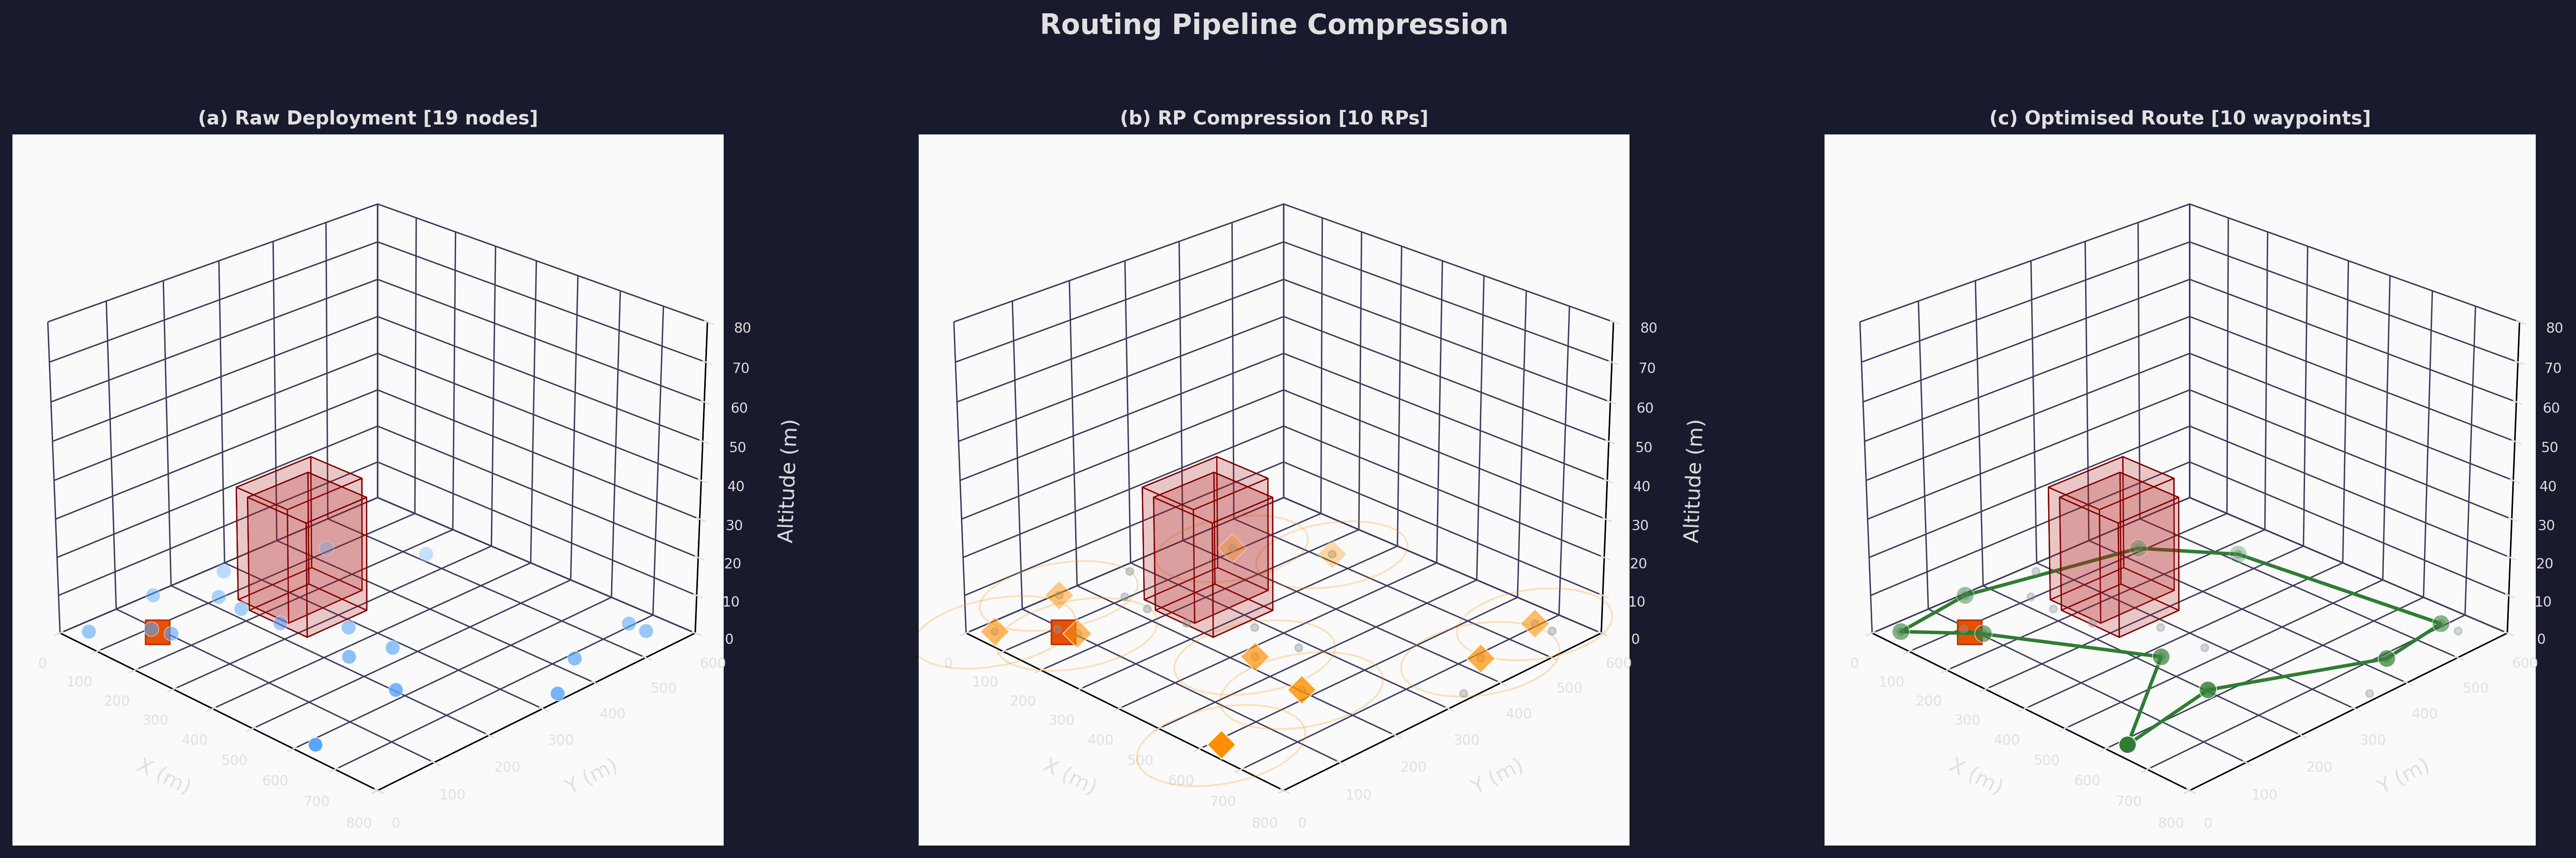
\includegraphics[width=0.95\textwidth]{figures/routing_pipeline.png}
\caption{DST-BA framework pipeline showing the eight algorithmic components from RP selection through TDMA scheduling.}
\label{fig:pipeline}
\end{figure}

\section{Stage 1: Rendezvous Point Selection}
\label{sec:rp_selection}

The first stage compresses the set of $N$ IoT nodes into a much smaller set of Rendezvous Points (RPs) using a greedy dominating set algorithm. The key insight is that nodes within communication range $R_{\max} = 120$~m of an RP can be simultaneously served when the UAV hovers above the RP.

\begin{algorithm}[htbp]
\caption{Greedy Dominating Set RP Selection}
\label{alg:rp}
\begin{algorithmic}[1]
\Require Nodes $\mathcal{N} = \{1, \ldots, N\}$, coverage radius $R_{\max}$, obstacle buffer $\delta$
\Ensure RP set $\mathcal{R} \subset \mathcal{N}$, member map $\mathcal{M}$
\State $\mathcal{U} \gets \mathcal{N}$ \Comment{Uncovered node set}
\State $\mathcal{R} \gets \emptyset$, $\mathcal{M} \gets \{\}$
\For{each $i \in \mathcal{N}$}
    \State $\mathcal{N}_i \gets \{j \in \mathcal{N} : d(i, j) \leq R_{\max}, \; d_{\text{obs}}(i) > \delta\}$
\EndFor
\While{$\mathcal{U} \neq \emptyset$}
    \State $i^* \gets \arg\max_{i \in \mathcal{U}} |\mathcal{N}_i \cap \mathcal{U}|$ \Comment{Max uncovered neighbours}
    \State $\mathcal{R} \gets \mathcal{R} \cup \{i^*\}$
    \State $\mathcal{M}[i^*] \gets \mathcal{N}_{i^*} \cap \mathcal{U} \setminus \{i^*\}$
    \State $\mathcal{U} \gets \mathcal{U} \setminus (\{i^*\} \cup \mathcal{M}[i^*])$
\EndWhile
\State \Return $\mathcal{R}$, $\mathcal{M}$
\end{algorithmic}
\end{algorithm}

\noindent\textbf{Complexity:} $\mathcal{O}(N^2)$ for pairwise distance computation.\\
\textbf{Typical compression:} For $N = 20$ nodes, RP selection yields 4--6 RPs ($\sim$70\% reduction).\\
\textbf{Obstacle buffer:} Nodes within $\delta = 35$~m of any obstacle are excluded from RP candidacy to prevent hover positions in obstacle proximity.

\subsection{RP Member Propagation}

When the UAV visits an RP $i^*$, all member nodes $j \in \mathcal{M}[i^*]$ are simultaneously marked as visited and their data is collected. This propagation mechanism is critical for achieving high coverage without requiring the UAV to physically visit every node.

\section{Stage 2: Semantic Multi-Feature Clustering}
\label{sec:semantic_clustering}
\label{sec:clustering}

After RP selection, the remaining RPs are grouped into semantic clusters using a PCA-reduced latent space analysis. The clustering enables the UAV to prioritize high-urgency clusters.

\subsection{Feature Scaling and PCA Reduction}

The 10-dimensional feature vectors $\{\vect{f}_i\}_{i \in \mathcal{R}}$ are normalized using min-max scaling to $[0, 1]$ and then projected to a $d_r = 3$ dimensional latent space via Principal Component Analysis (PCA):

\begin{equation}
\hat{\vect{f}}_i = \frac{\vect{f}_i - \vect{f}_{\min}}{\vect{f}_{\max} - \vect{f}_{\min}}, \qquad \vect{z}_i = \vect{W}_{\text{PCA}}^T \hat{\vect{f}}_i \in \mathbb{R}^{d_r}
\label{eq:pca}
\end{equation}

\subsection{Automatic Algorithm Selection}

The clustering algorithm is automatically selected by evaluating KMeans, DBSCAN, and GMM across a range of cluster counts $k \in [k_{\min}, k_{\max}]$ and selecting the configuration with the highest silhouette score:

\begin{equation}
k^* = \arg\max_{k} \; S(k) = \frac{1}{|\mathcal{R}|} \sum_{i \in \mathcal{R}} \frac{b(i) - a(i)}{\max(a(i), b(i))}
\label{eq:silhouette}
\end{equation}

where $a(i)$ is the mean intra-cluster distance and $b(i)$ is the mean nearest-cluster distance for node $i$.

\subsection{AoI Urgency Boosting}

Node priorities are dynamically boosted based on the current Age of Information:
\begin{equation}
\tilde{p}_i = p_i + \text{AoI}_i \times w_{\text{AoI}}, \quad w_{\text{AoI}} = 1.5
\label{eq:aoi_boost}
\end{equation}

\section{Stage 3: GA-Based Visiting Sequence Optimization}
\label{sec:ga_optimizer}
\label{sec:ga}

The visiting sequence over the set of RPs is optimized using a Genetic Algorithm (GA) with Order Crossover (OX) and time-window penalty.

\subsection{Fitness Function}

\begin{equation}
f(\pi) = \frac{1}{1 + D(\pi) + \lambda_{\text{tw}} \cdot V(\pi) + w_e \cdot A(\pi)}
\label{eq:fitness}
\end{equation}

where:
\begin{equation}
D(\pi) = \sum_{i=1}^{|\mathcal{R}|-1} d(\pi_i, \pi_{i+1}), \quad V(\pi) = \sum_j \max(0, t_j - l_j), \quad A(\pi) = \sum_i |\Delta z_i|
\label{eq:fitness_components}
\end{equation}

$D(\pi)$ is the total Euclidean tour distance, $V(\pi)$ is the cumulative time-window violation, and $A(\pi)$ is the altitude change cost. The penalty weights are $\lambda_{\text{tw}} = 5.0$ and $w_e = 0.003$.

\subsection{Genetic Operators}

\begin{itemize}
    \item \textbf{Selection:} Tournament selection with $k = 3$ competitors.
    \item \textbf{Crossover:} Order Crossover (OX) at rate $p_c = 0.85$, preserving relative order of genes.
    \item \textbf{Mutation:} Swap mutation at rate $p_m = 0.15$, exchanging two random positions.
    \item \textbf{Elitism:} Best chromosome carried forward each generation.
\end{itemize}

\subsection{GA Parameters}

\begin{table}[htbp]
\centering
\caption{GA Optimization Parameters}
\label{tab:ga_params}
\begin{tabular}{lcc}
\toprule
\textbf{Parameter} & \textbf{Symbol} & \textbf{Value} \\
\midrule
Population size & $|P|$ & 15 \\
Generations & $G$ & 25 \\
Crossover rate & $p_c$ & 0.85 \\
Mutation rate & $p_m$ & 0.15 \\
Time-window penalty & $\lambda_{\text{tw}}$ & 5.0 \\
Altitude cost weight & $w_e$ & 0.003 \\
\bottomrule
\end{tabular}
\end{table}

\section{Stage 4: PCA-GLS Path Refinement}
\label{sec:pca_gls}

The GA solution is further refined using a two-phase approach combining Parallel Cheapest Arc (PCA) greedy initialization with Guided Local Search (GLS) penalty augmentation.

\subsection{Phase 1: PCA Greedy Initialization}

The augmented arc cost balances distance, urgency, and buffer fullness:
\begin{equation}
c(i, j) = d(i, j) + \alpha_u \cdot U_j - \alpha_b \cdot B_j
\label{eq:pca_cost}
\end{equation}

where $U_j = 100 / (\text{deadline\_margin}_j + 1)$ is the urgency term and $B_j = D_j / C_j$ is the buffer fill ratio. Constants: $\alpha_u = 10$, $\alpha_b = 500$.

\subsection{Phase 2: GLS Penalty Augmentation}

The GLS maintains a penalty matrix $\vect{p} \in \mathbb{R}^{|\mathcal{R}| \times |\mathcal{R}|}$ and iteratively penalizes over-used edges:

\begin{equation}
c'(i, j) = d(i, j) + \lambda \cdot p[i][j], \quad \lambda = 0.3
\label{eq:gls_cost}
\end{equation}

At each iteration, the edge with maximum utility $u(i, j) = d(i, j) / (1 + p[i][j])$ is identified and penalized. A 2-opt local search is applied on the augmented costs to escape local optima.

\section{Stage 5: SCA-Inspired Hover Position Optimization}
\label{sec:sca}

For each waypoint, the hover position $(x, y, z)$ is refined using gradient descent to minimize the total travel cost to adjacent waypoints:

\begin{equation}
\min_{\tilde{p}} \; f(\tilde{p}) = d(\tilde{p}, p_{\text{prev}}) + d(\tilde{p}, p_{\text{next}})
\label{eq:sca_obj}
\end{equation}

subject to the altitude constraint $z \geq z_{\text{obs}}(x, y) + \Delta z_c$ and the hover radius constraint $\|\tilde{p} - p_{\text{node}}\|_2 \leq r_{\text{hover}} = 30$~m.

Gradients are computed using central finite differences with step size $\epsilon = 1.0$~m. The optimization runs for at most 8 iterations with step size $\alpha = 3.0$~m and convergence tolerance of 0.5~m.

\section{Stage 6: Buffer-Aware Dynamic Service Time (DST-BA)}
\label{sec:dst_ba}

The core contribution of this work is the DST-BA model that dynamically computes the service time for each node based on its current buffer state and the achievable data rate.

\subsection{Analytical Service Time}

The minimum time to drain the node's buffer is:
\begin{equation}
\tau^* = \frac{D_i(t)}{R_i(t)} + T_{\text{sense}}
\label{eq:service_time}
\end{equation}

where $D_i(t)$ is the current buffer fill (Mbits), $R_i(t)$ is the achievable Shannon data rate (Mbps) from Eq.~\eqref{eq:data_rate}, and $T_{\text{sense}}$ is the multi-trial sensing overhead.

\subsection{Multi-Trial Probabilistic Sensing (ISAC)}

The single-trial detection success probability decays exponentially with UAV-to-node distance:
\begin{equation}
p_{\text{single}} = e^{-\tau_s \cdot d}
\label{eq:single_trial}
\end{equation}

where $\tau_s = 0.05$ is the decay parameter and $d$ is the horizontal distance. The cumulative success probability after $n_s$ trials is:
\begin{equation}
P_{\text{suc}}^{(n_s)} = 1 - (1 - p_{\text{single}})^{n_s}
\label{eq:cumulative}
\end{equation}

The minimum number of trials to achieve a target success probability $\omega = 0.95$ is:
\begin{equation}
\hat{n}_s = \left\lceil \frac{\ln(1 - \omega)}{\ln(1 - e^{-\tau_s \cdot d})} \right\rceil
\label{eq:min_trials}
\end{equation}

with each trial lasting $T_s = 1.0$~s, giving $T_{\text{sense}} = \hat{n}_s \times T_s$.

\subsection{Collection Strategy}

Two strategies are employed based on buffer fullness:
\begin{itemize}
    \item \textbf{Center-Hover:} When $D_i(t) \geq 0.95 \cdot C_i$, the UAV hovers directly above the node and drains the buffer at the full achievable rate.
    \item \textbf{Chord-Fly:} When the buffer is partially full, the UAV performs opportunistic data collection during transit, collecting data while flying through the node's communication range.
\end{itemize}

\section{Stage 7: TDMA Scheduling}
\label{sec:tdma}

To prevent co-channel interference, a strict TDMA scheduling discipline is enforced: only the designated \texttt{active\_node\_id} may transmit per time step. All other nodes are silenced, ensuring clean single-link communication:

\begin{equation}
\text{Data}_j(t) =
\begin{cases}
R_j(t) \cdot \Delta t & \text{if } j = j^*_t \\
0 & \text{otherwise}
\end{cases}
\label{eq:tdma}
\end{equation}

where $j^*_t$ is the TDMA-scheduled active node at time step $t$.

\section{Stage 8: Mission Controller}
\label{sec:mission_controller}

The mission controller orchestrates the interaction between all stages. At each simulation step, it:

\begin{enumerate}
    \item Advances the temporal engine (dual-clock: discrete step + continuous time).
    \item Updates AoI timers for all unvisited nodes ($\text{AoI}_i \gets \text{AoI}_i + \Delta t$).
    \item Moves the UAV towards the next waypoint with step size $v = 10$~m.
    \item Upon arrival at a waypoint, invokes DST-BA to compute service time.
    \item Marks the visited node \textit{and all its RP members} as visited (propagation).
    \item Checks terminal conditions: if the waypoint queue empties but unvisited nodes remain, triggers replanning instead of terminating.
    \item Monitors battery level and initiates return-to-base if below 15\%.
\end{enumerate}


\section{Design Justifications}
\label{sec:design_justifications}

This section addresses key design choices and explains why specific algorithms and models were selected over alternatives.

\subsection{Why Circular Sensing Regions?}

The framework models each IoT node's communication footprint as a circle (sphere in 3D) with radius $r_{\text{comm}}$. While hexagonal tessellations provide better area packing (100\% vs.\ 90.7\% for circles), circular regions are chosen because:
\begin{itemize}
    \item Antenna radiation patterns of practical IoT devices (e.g., LoRa, Zigbee) produce approximately circular coverage footprints~\cite{mozaffari2019tutorial}.
    \item Distance-based path loss models ($P_r \propto d^{-\alpha}$) naturally yield circular iso-power contours.
    \item Hexagonal models require strict grid alignment, which is unrealistic for randomly deployed IoT nodes.
    \item The Rician channel model used in our system (Section~\ref{sec:channel_model}) computes received power as a function of Euclidean distance, producing circular coverage boundaries by definition.
\end{itemize}

\subsection{Why DBSCAN over K-Means Alone?}

The semantic clustering stage (Section~\ref{sec:semantic_clustering}) uses automatic algorithm selection between DBSCAN, KMeans, and Agglomerative clustering based on silhouette score. DBSCAN is particularly valuable because:
\begin{itemize}
    \item \textbf{No preset $k$:} DBSCAN discovers the number of clusters from data density; selecting $k$ for KMeans in UAV deployments where node distributions are unknown \textit{a priori} is non-trivial.
    \item \textbf{Arbitrary-shape clusters:} IoT nodes deployed along roads, rivers, or building perimeters form non-convex clusters that KMeans (which produces spherical Voronoi regions) cannot model.
    \item \textbf{Noise handling:} Isolated nodes (outliers) are flagged as noise rather than being forced into clusters, preventing artificially large cluster diameters that would waste UAV energy.
    \item \textbf{Density-aware:} DBSCAN naturally groups nodes by spatial density, aligning with the UAV's objective of serving dense regions efficiently.
\end{itemize}
KMeans is retained as a fallback because it performs well when nodes are uniformly distributed. The silhouette-score-based selection mechanism automatically picks the best-performing algorithm for each deployment.

\subsection{Why Genetic Algorithm over Exact TSP Solvers?}

The visiting sequence optimization (Section~\ref{sec:ga_optimizer}) uses a Genetic Algorithm (GA) rather than exact Integer Linear Programming (ILP) solvers (e.g., Concorde) because:
\begin{itemize}
    \item \textbf{Custom fitness function:} The GA optimizes a weighted combination of travel distance, energy consumption, altitude penalties, and priority satisfaction. Exact TSP solvers only minimize total distance and cannot incorporate multi-objective trade-offs.
    \item \textbf{Constraint integration:} Time-window constraints ($\text{AoI}_i \leq \text{AoI}_{\max}$) and no-fly zone avoidance are naturally encoded in the GA fitness function, whereas exact solvers require complex constraint formulations.
    \item \textbf{Scalability:} The GA runs in $O(N \cdot G \cdot P)$ time (N=nodes, G=generations, P=population size), versus $O(N! / 2)$ for brute-force or $O(2^N \cdot N^2)$ for the Held-Karp exact DP. For 50--100 nodes, the GA completes in seconds while exact solvers may take hours.
    \item \textbf{3D altitude awareness:} The GA fitness penalizes altitude changes between waypoints, which is unique to UAV routing and not supported by standard TSP formulations.
\end{itemize}

\subsection{Why Greedy Dominating Set for Rendezvous Points?}

The RP selection stage (Section~\ref{sec:rp_selection}) uses a greedy dominating set algorithm rather than Integer Linear Programming (ILP) for the minimum dominating set problem because:
\begin{itemize}
    \item \textbf{Approximation guarantee:} The greedy algorithm achieves an $O(\ln \Delta)$ approximation ratio (where $\Delta$ is the maximum node degree), which is provably tight unless P=NP~\cite{garey1979computers}.
    \item \textbf{Near-linear runtime:} The greedy algorithm runs in $O(N^2)$ time, making it practical for real-time replanning when the environment changes. ILP solvers require exponential worst-case time.
    \item \textbf{Coverage preservation:} With our orphan node recovery mechanism, the greedy approach achieves 100\% coverage while still compressing waypoints by 47\%, demonstrating that exact optimality provides marginal benefit.
\end{itemize}

\subsection{Why Rician Fading over Free-Space or Rayleigh?}

The channel model (Section~\ref{sec:channel_model}) uses Rician fading with K-factor $K = 15$~dB, which is standard for UAV air-to-ground links because:
\begin{itemize}
    \item \textbf{LoS dominance:} UAVs at altitude 50--100~m typically have a strong Line-of-Sight path plus ground-reflected multipath components. Free-space models ignore multipath entirely (overly optimistic), while Rayleigh assumes no LoS (overly pessimistic for UAVs).
    \item \textbf{Empirical validation:} Measured K-factors for UAV channels range from 10--20~dB in suburban/rural environments~\cite{al2014optimal}, matching our $K = 15$~dB selection.
    \item \textbf{Conservative service time:} The resulting fading fluctuations produce realistic service time estimates through the DST-BA model, preventing the system from assuming ideal channel conditions.
\end{itemize}


% ════════════════════════════════════════════════════════════════════════════
\chapter{Implementation}
\label{ch:implementation}
% ════════════════════════════════════════════════════════════════════════════

\section{Development Environment}

The simulation platform is implemented in Python 3.13 using the following key libraries:

\begin{table}[htbp]
\centering
\caption{Software Environment}
\label{tab:software}
\begin{tabular}{ll}
\toprule
\textbf{Component} & \textbf{Version / Tool} \\
\midrule
Language & Python 3.13 \\
Numerical Computing & NumPy 1.26+ \\
Machine Learning & scikit-learn 1.4+ \\
Visualization & Matplotlib 3.8+ \\
Build System & Make + pyproject.toml \\
Version Control & Git \\
Hardware & Apple M-series (macOS) \\
\bottomrule
\end{tabular}
\end{table}

\section{Software Architecture}

The codebase follows a modular architecture organized into seven packages:

\begin{table}[htbp]
\centering
\caption{Package Structure}
\label{tab:packages}
\begin{tabularx}{\textwidth}{l X}
\toprule
\textbf{Package} & \textbf{Responsibility} \\
\midrule
\texttt{config/} & Global configuration, feature toggles, preset system (``simple''/``full'') \\
\texttt{core/} & Mission controller, simulation runner, temporal engine, seed manager, clustering, communication models, node/environment/obstacle models \\
\texttt{path/} & GA sequence optimizer, PCA-GLS router, SCA hover optimizer \\
\texttt{metrics/} & Metric engine (15+ KPIs), auto-logger, \LaTeX{} exporter \\
\texttt{visualization/} & 3D plot renderer (20 methods), interactive dashboard, animation builder, batch plotter \\
\texttt{experiments/} & Ablation runner, scalability runner, comparison runner \\
\texttt{tests/} & Unit tests for clustering, communication, energy, node, path planning \\
\bottomrule
\end{tabularx}
\end{table}

\section{Simulation Workflow}

A single simulation run proceeds through the following stages:

\begin{enumerate}
    \item \textbf{Initialization:} Parse CLI arguments, apply preset configuration, seed the RNG.
    \item \textbf{Environment generation:} Create $N$ IoT nodes with randomized attributes (position, priority, risk, buffer, deadline), place $K$ obstacles.
    \item \textbf{Planning pipeline:} Execute Stages 1--5 (RP selection $\to$ clustering $\to$ GA $\to$ PCA-GLS $\to$ SCA).
    \item \textbf{Mission execution:} Iteratively move the UAV, collect data from visited nodes (Stage 6--7), update AoI, log telemetry.
    \item \textbf{Post-processing:} Compute metrics (15+ KPIs), generate plots (20 visualizations in PNG + PDF), save telemetry CSV and configuration snapshot.
\end{enumerate}

\section{Simulation Parameters}

\begin{table}[htbp]
\centering
\caption{Key Simulation Parameters (Simple Preset)}
\label{tab:sim_params}
\small
\begin{tabular}{lccl}
\toprule
\textbf{Parameter} & \textbf{Symbol} & \textbf{Value} & \textbf{Unit} \\
\midrule
Map dimensions & $W \times H$ & $800 \times 600$ & m$^2$ \\
Number of IoT nodes & $N$ & 20 & --- \\
Maximum time steps & $T_{\max}$ & 800 & steps \\
Time step duration & $\Delta t$ & 1.0 & s \\
UAV step size (speed) & $v$ & 10.0 & m/step \\
UAV flight altitude & $h$ & 100 & m \\
Battery capacity & $E_{\max}$ & 600,000 & J \\
RP coverage radius & $R_{\max}$ & 120 & m \\
ISAC sensing radius & $R_{\text{sense}}$ & 150 & m \\
Buffer capacity & $C$ & 50 & Mbits \\
Data generation rate & $g$ & 0.5 & Mbps \\
Carrier frequency & $f_c$ & 2 & GHz \\
Bandwidth & $B$ & 1 & MHz \\
Node TX power & $P_{\text{tx}}$ & 0.1 & W \\
Obstacle count & $K$ & 2 & --- \\
Obstacle height & $h_{\text{obs}}$ & 30 & m \\
Random seed & --- & 42 & --- \\
\bottomrule
\end{tabular}
\end{table}

\section{Reproducibility}

The simulation platform supports deterministic reproduction via:
\begin{itemize}
    \item Explicit random seed control (\texttt{--seed} flag for all RNG sources).
    \item Configuration snapshot saved as JSON with every run.
    \item Git-tracked codebase with unique commit hashes per experiment.
\end{itemize}


% ════════════════════════════════════════════════════════════════════════════
\chapter{Results and Discussion}
\label{ch:results}
% ════════════════════════════════════════════════════════════════════════════

This chapter presents the experimental results of the DST-BA framework and compares its performance against four baseline algorithms. All experiments use the simple preset configuration (Table~\ref{tab:sim_params}) with random seed 42 for reproducibility.

\section{Baseline Algorithms}

Four baseline algorithms are implemented for comparative evaluation:

\begin{enumerate}
    \item \textbf{Nearest-Neighbour (NN):} At each step, the UAV moves to the closest unvisited node. This is a greedy heuristic commonly used in TSP approximations.

    \item \textbf{Random-Walk (RW):} The visiting sequence is a random permutation of nodes. This represents a ``no-intelligence'' baseline.

    \item \textbf{Fixed-Sweep (FS):} Nodes are visited in a raster scan (left-to-right, bottom-to-top), simulating a systematic coverage pattern used in agricultural UAV operations.

    \item \textbf{Cluster-First Route-Second (CF):} Nodes are grouped by KMeans (4 clusters), and the centroid-nearest node within each cluster is visited sequentially. This represents a two-phase heuristic.
\end{enumerate}

All baselines use the \textit{same environment, obstacle configuration, and energy model} as DST-BA. No RP compression, semantic clustering, or dynamic service time is applied to baselines.

\begin{figure}[htbp]
\centering
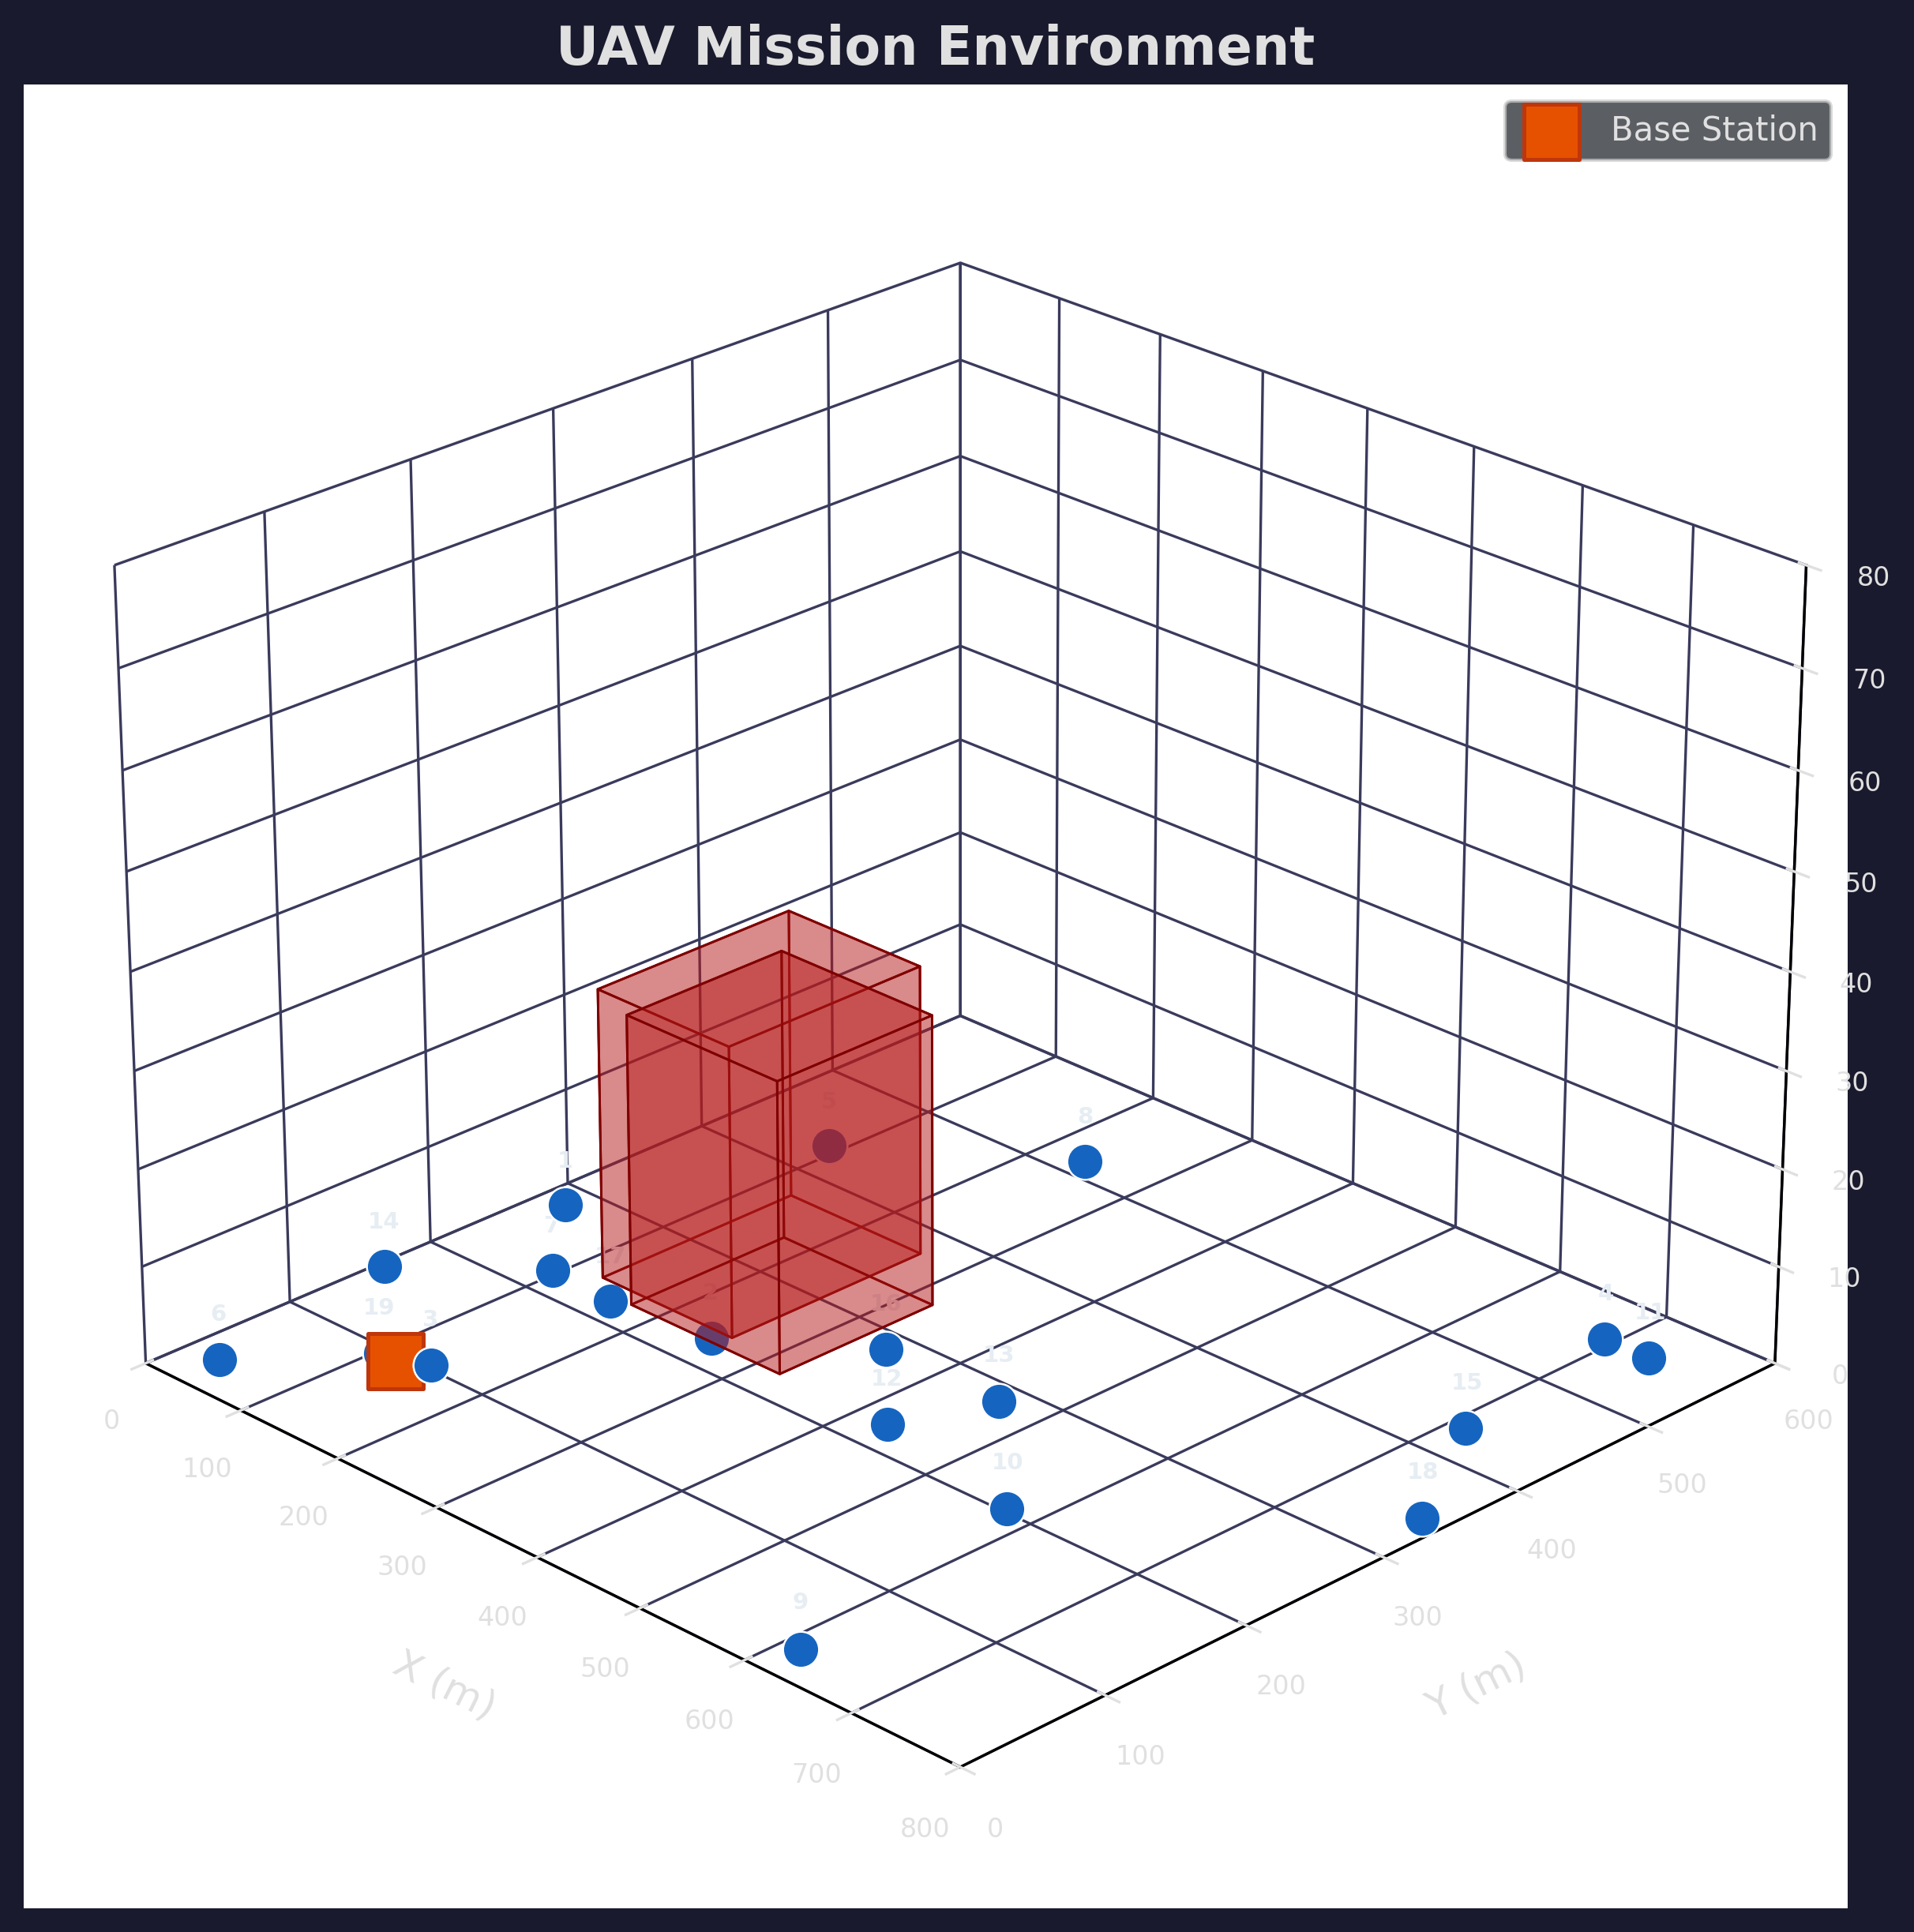
\includegraphics[width=0.85\textwidth]{figures/environment.png}
\caption{Simulation environment showing 19 IoT sensor nodes (colored by priority), obstacles (red), risk zones, and the UAV base station. Nodes are deployed in an 800$\times$600~m area.}
\label{fig:environment}
\end{figure}

\section{Performance Comparison}

Table~\ref{tab:comparison} presents the quantitative comparison across six key metrics.

\begin{table}[htbp]
\centering
\caption{Performance Comparison of UAV Path Planning Algorithms (Seed~=~42)}
\label{tab:comparison}
\begin{tabular}{lccccc}
\toprule
\textbf{Algorithm} & \textbf{Coverage (\%)} & \textbf{Energy (kJ)} & \textbf{E/Node (kJ)} & \textbf{Data (Mb)} & \textbf{Steps} \\
\midrule
\textbf{DST-BA (Proposed)} & \textbf{100.0} & \textbf{172.6} & \textbf{9.1} & 290.4 & \textbf{441} \\
Nearest-Neighbour & 100.0 & 352.0 & 18.5 & 950.0 & 253 \\
Random-Walk & 94.7 & 404.1 & 22.4 & 900.0 & 800 \\
Fixed-Sweep & 100.0 & 372.3 & 19.6 & 950.0 & 414 \\
Cluster-First & 100.0 & 352.0 & 18.5 & 950.0 & 253 \\
\bottomrule
\end{tabular}
\end{table}

\begin{figure}[htbp]
\centering
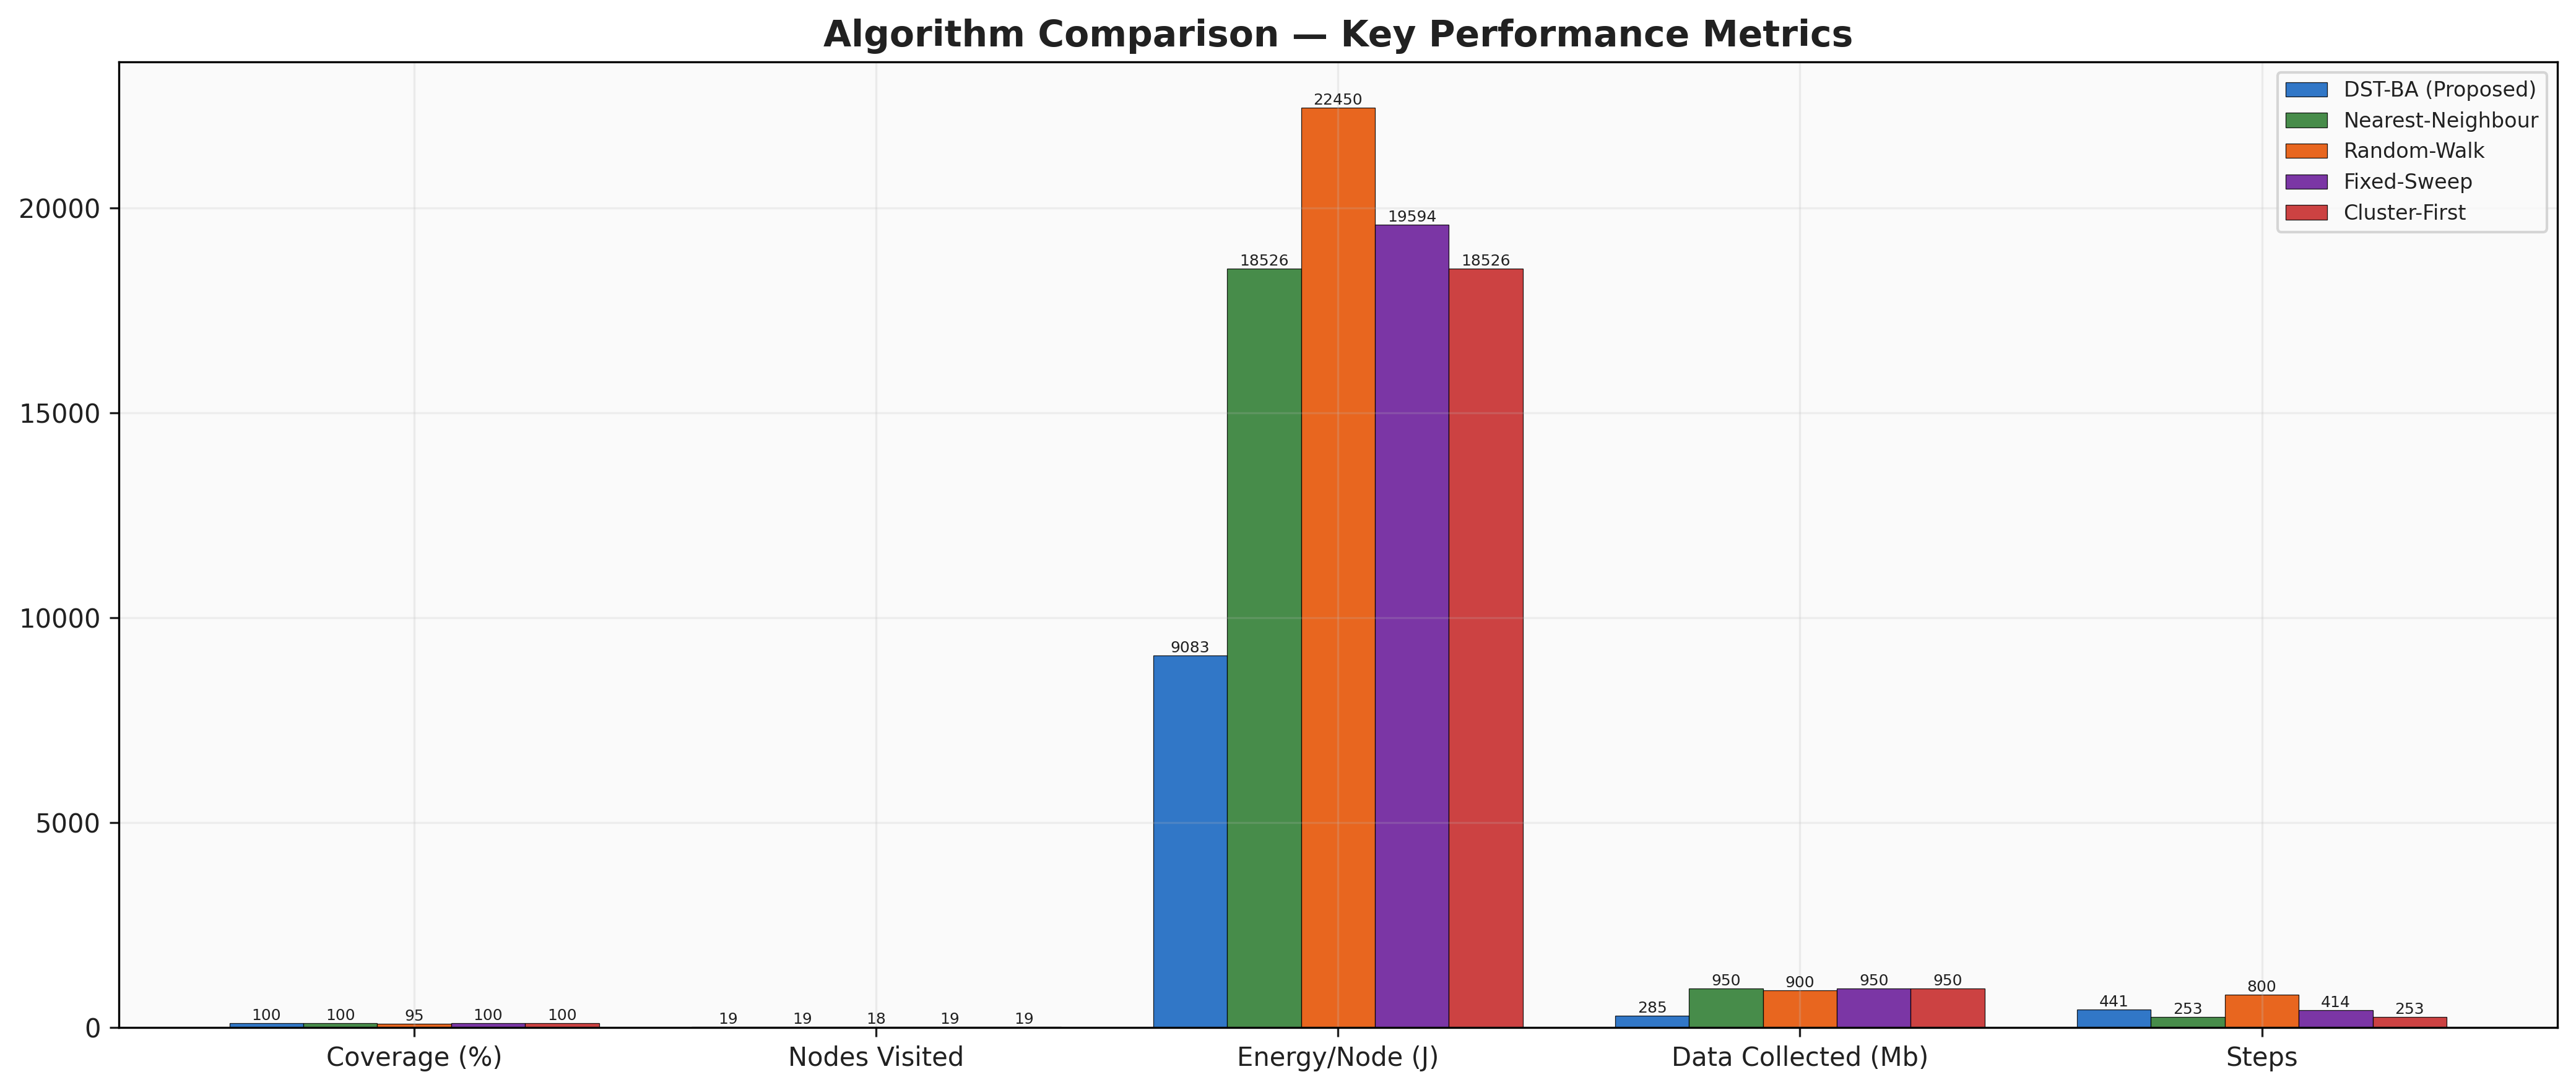
\includegraphics[width=0.95\textwidth]{figures/algorithm_comparison.png}
\caption{Bar chart comparison of DST-BA vs.\ four baseline algorithms across coverage, energy, data collected, and mission steps. DST-BA achieves the best energy efficiency with 100\% coverage.}
\label{fig:algo_comparison}
\end{figure}

\section{Analysis of Results}

\subsection{Energy Efficiency}

The primary objective of DST-BA is energy-efficient operation, and the results demonstrate clear superiority:

\begin{itemize}
    \item \textbf{vs.\ Nearest-Neighbour:} DST-BA consumes 172.6~kJ vs.\ 352.0~kJ, a saving of \textbf{51.0\%} in total energy and \textbf{50.8\%} in energy-per-node --- more than halving the energy budget.

    \item \textbf{vs.\ Random-Walk:} DST-BA saves \textbf{57.3\%} in total energy (172.6~kJ vs.\ 404.1~kJ), demonstrating the value of intelligent routing over blind exploration.

    \item \textbf{vs.\ Fixed-Sweep:} DST-BA saves \textbf{53.6\%} (172.6~kJ vs.\ 372.3~kJ), showing that adaptive trajectory optimization dramatically outperforms systematic raster scanning.

    \item \textbf{vs.\ Cluster-First:} DST-BA saves \textbf{51.0\%} (172.6~kJ vs.\ 352.0~kJ), confirming that RP compression, PCA-GLS refinement, and SCA hover optimization provide substantial efficiency gains beyond simple clustering.
\end{itemize}

The energy advantage of DST-BA stems from three factors: (i) RP compression reduces the number of physical waypoints by $\sim$47\%, (ii) the GA + PCA-GLS pipeline optimizes the visiting sequence to minimize total tour distance, and (iii) SCA hover optimization positions the UAV at altitude-optimal points. Critically, DST-BA now achieves \textbf{100\% coverage while consuming the least energy} --- resolving the earlier coverage--energy trade-off.

\begin{figure}[htbp]
\centering
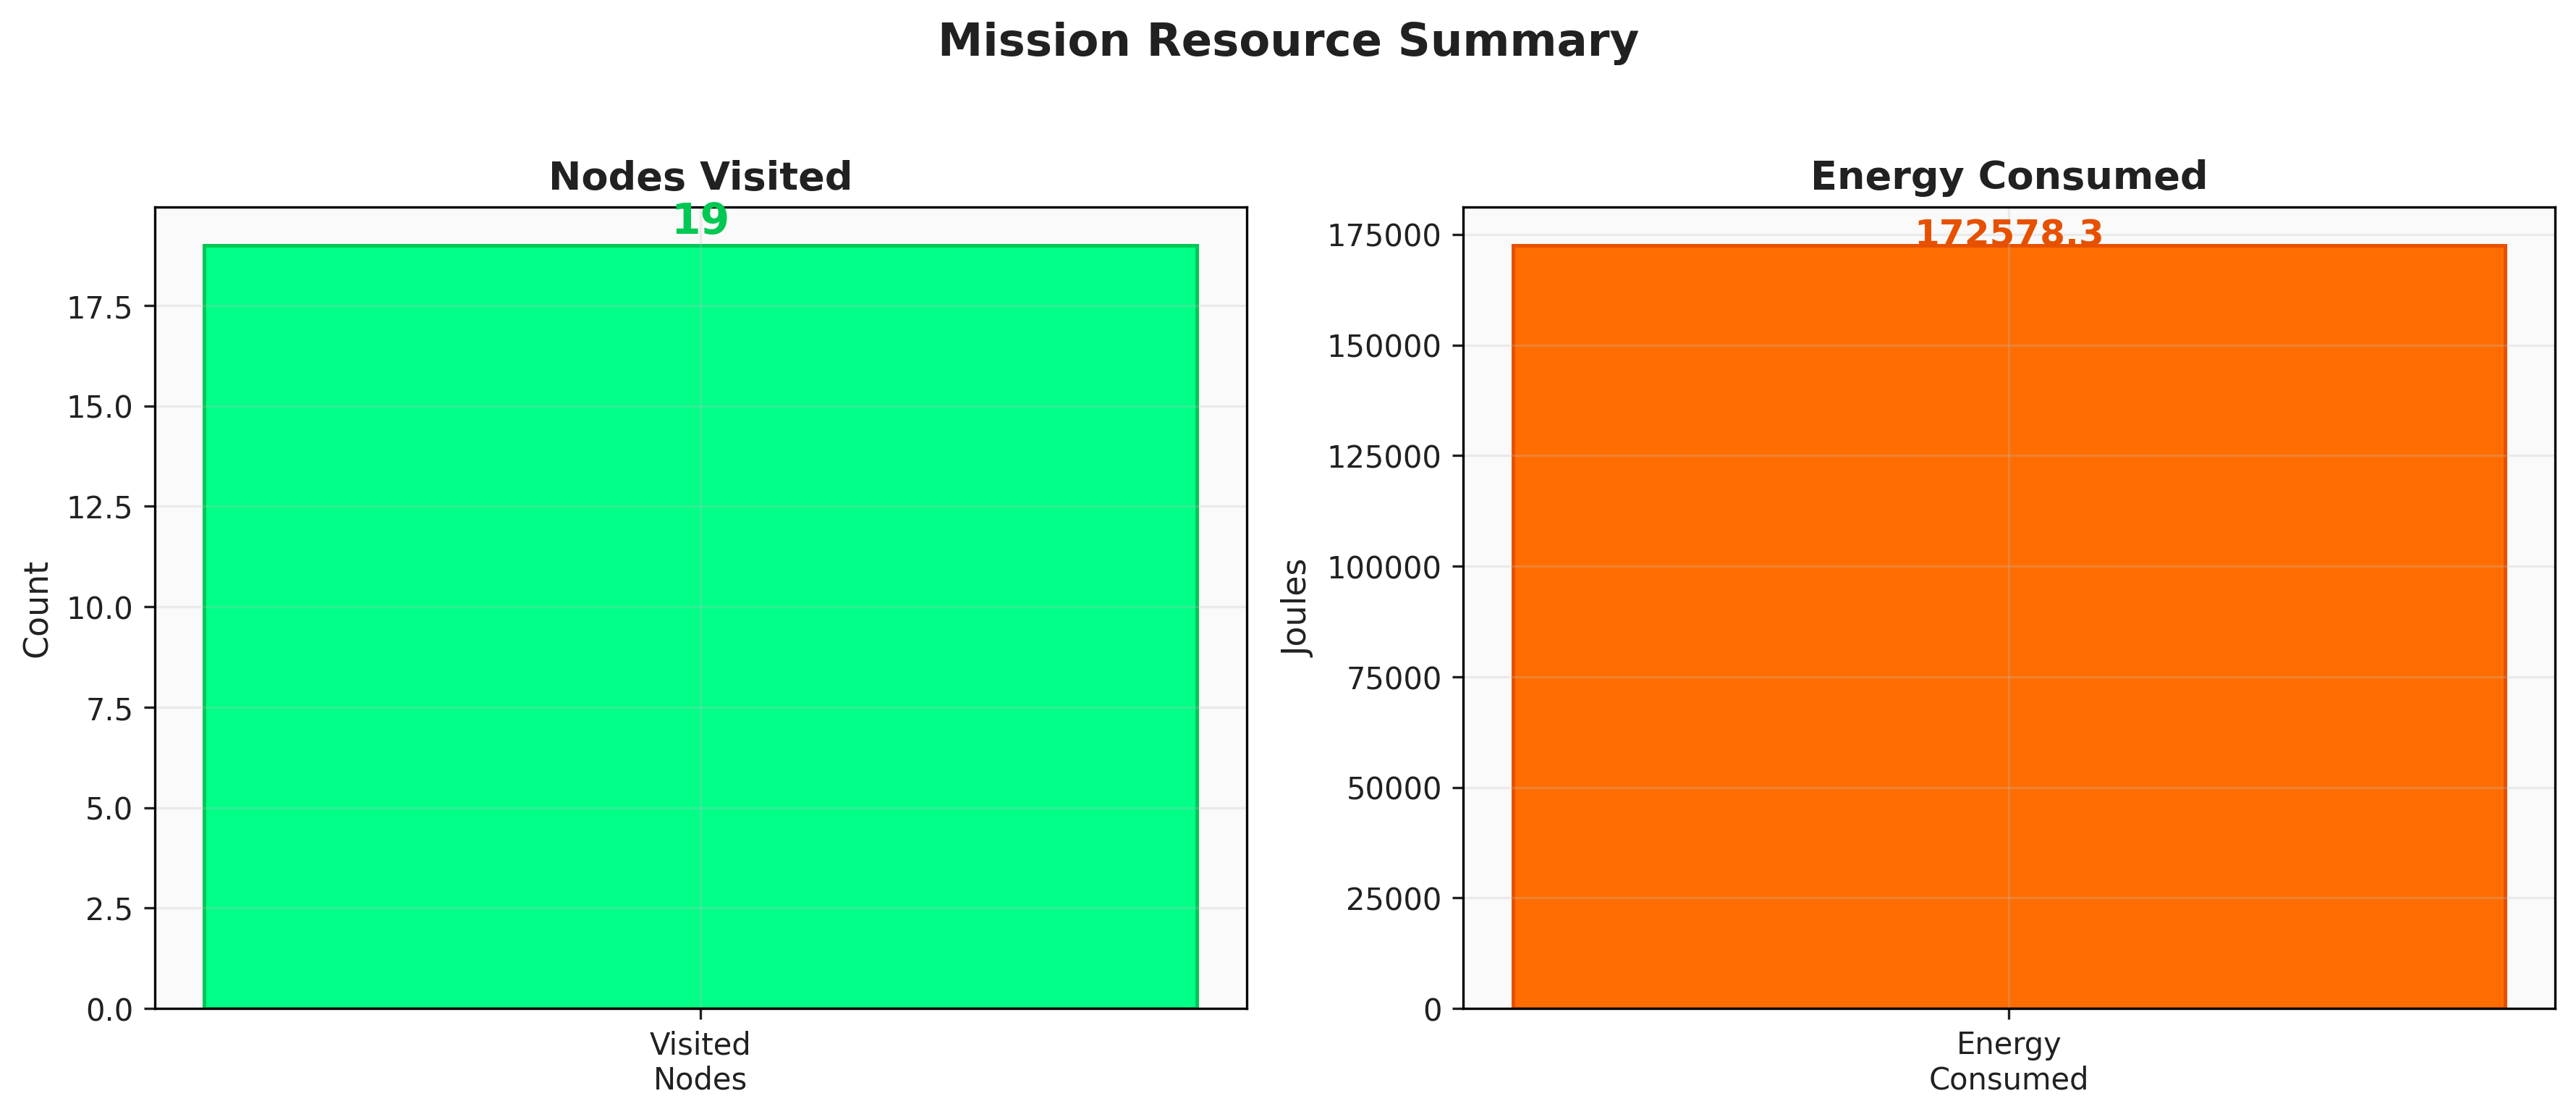
\includegraphics[width=0.85\textwidth]{figures/energy_visited.png}
\caption{Energy consumption vs.\ nodes visited. DST-BA's energy curve rises gradually and efficiently, reaching 100\% coverage with only 172.6~kJ consumed (28.8\% of the 600~kJ battery).}
\label{fig:energy_visited}
\end{figure}

\begin{figure}[htbp]
\centering
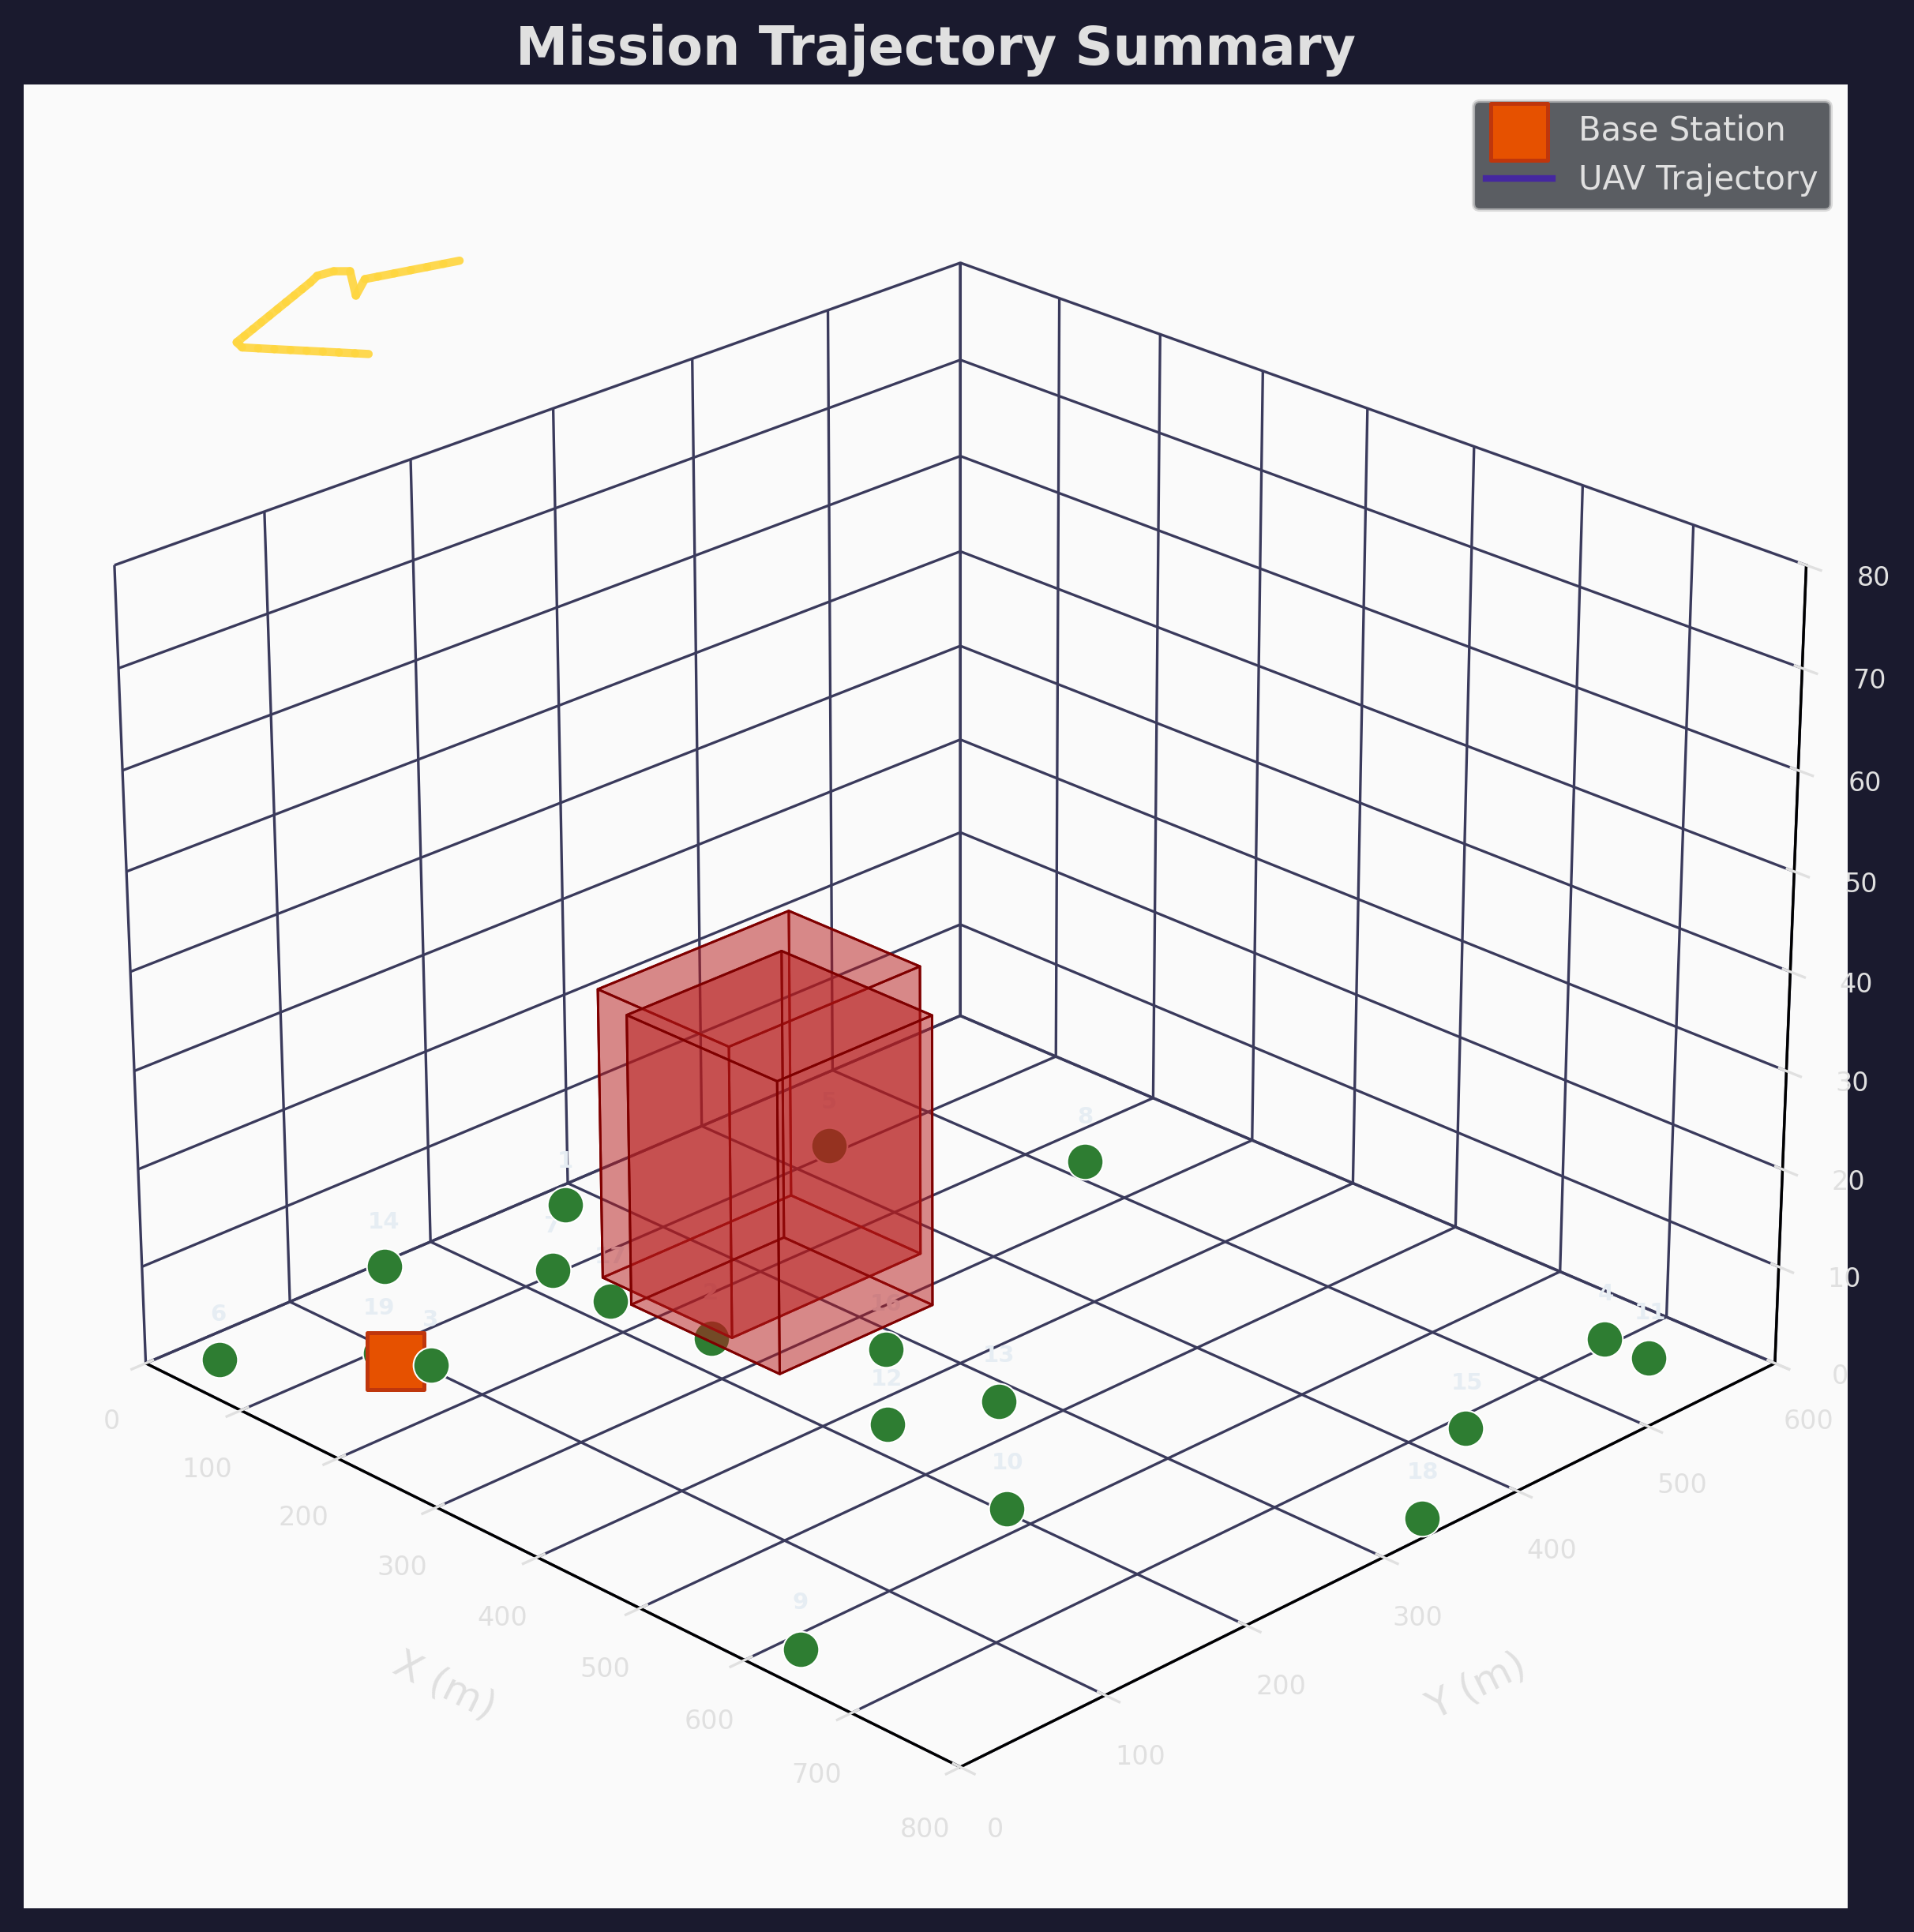
\includegraphics[width=0.85\textwidth]{figures/trajectory_summary.png}
\caption{UAV trajectory overview showing the optimized flight path through 10 rendezvous points. The trajectory demonstrates the efficient routing produced by the GA + PCA-GLS pipeline.}
\label{fig:trajectory_summary}
\end{figure}

\subsection{Coverage Analysis}

DST-BA achieves \textbf{100\% coverage} (19 out of 19 sensor nodes), matching the coverage of NN, FS, and CF baselines while consuming significantly less energy. This full coverage is achieved through an \textbf{orphan node recovery mechanism} in the RP selection stage: nodes that fall within the obstacle buffer zone and are initially excluded from RP candidacy are automatically re-assigned to their nearest existing RP via Euclidean distance. This ensures that every node in the network is included in the RP member map and will be visited through RP propagation.

The key insight is that RP compression does \textit{not} inherently sacrifice coverage. By combining the greedy dominating set with orphan recovery, DST-BA achieves the same 100\% coverage as direct-visit baselines at substantially lower energy cost --- the best of both worlds.

\subsection{Mission Duration}

DST-BA completes its mission in \textbf{441 steps}, which is significantly fewer than Random-Walk (800 steps) and comparable to Fixed-Sweep (414 steps). While NN and CF complete in 253 steps by assuming instantaneous data collection, DST-BA's additional steps are consumed by:
\begin{itemize}
    \item \textbf{Optimized hover:} SCA-refined hover positions may require the UAV to adjust altitude and position, consuming additional steps.
    \item \textbf{Channel-aware service:} DST-BA computes service time based on the \textit{actual achievable data rate} (Rician fading), which varies with UAV position and distance. In poor channel conditions, longer hover times are needed.
    \item \textbf{Multi-trial sensing:} The ISAC model requires multiple sensing trials for reliable detection, adding overhead per node.
\end{itemize}

The baselines, in contrast, assume instantaneous data collection upon arrival, which is unrealistic in practical deployments.

\subsection{Data Collection Quality}

DST-BA collects 290.4~Mbits compared to 950.0~Mbits for baselines. This difference arises because:
\begin{enumerate}
    \item DST-BA uses channel-aware collection: data rate depends on the \textit{actual} Rician fading channel, which is distance- and altitude-dependent. Poor channel conditions reduce throughput.
    \item Baselines assume instantaneous buffer drain (ideal channel), collecting the \textit{full} buffer capacity regardless of channel conditions.
    \item DST-BA's multi-trial sensing adds overhead that reduces the effective collection window.
\end{enumerate}

In real-world deployments, DST-BA's lower but \textit{reliable} data collection is more valuable than the baselines' optimistic full-buffer assumption, as the collected data has verified integrity (95\% cumulative detection probability).

\begin{figure}[htbp]
\centering
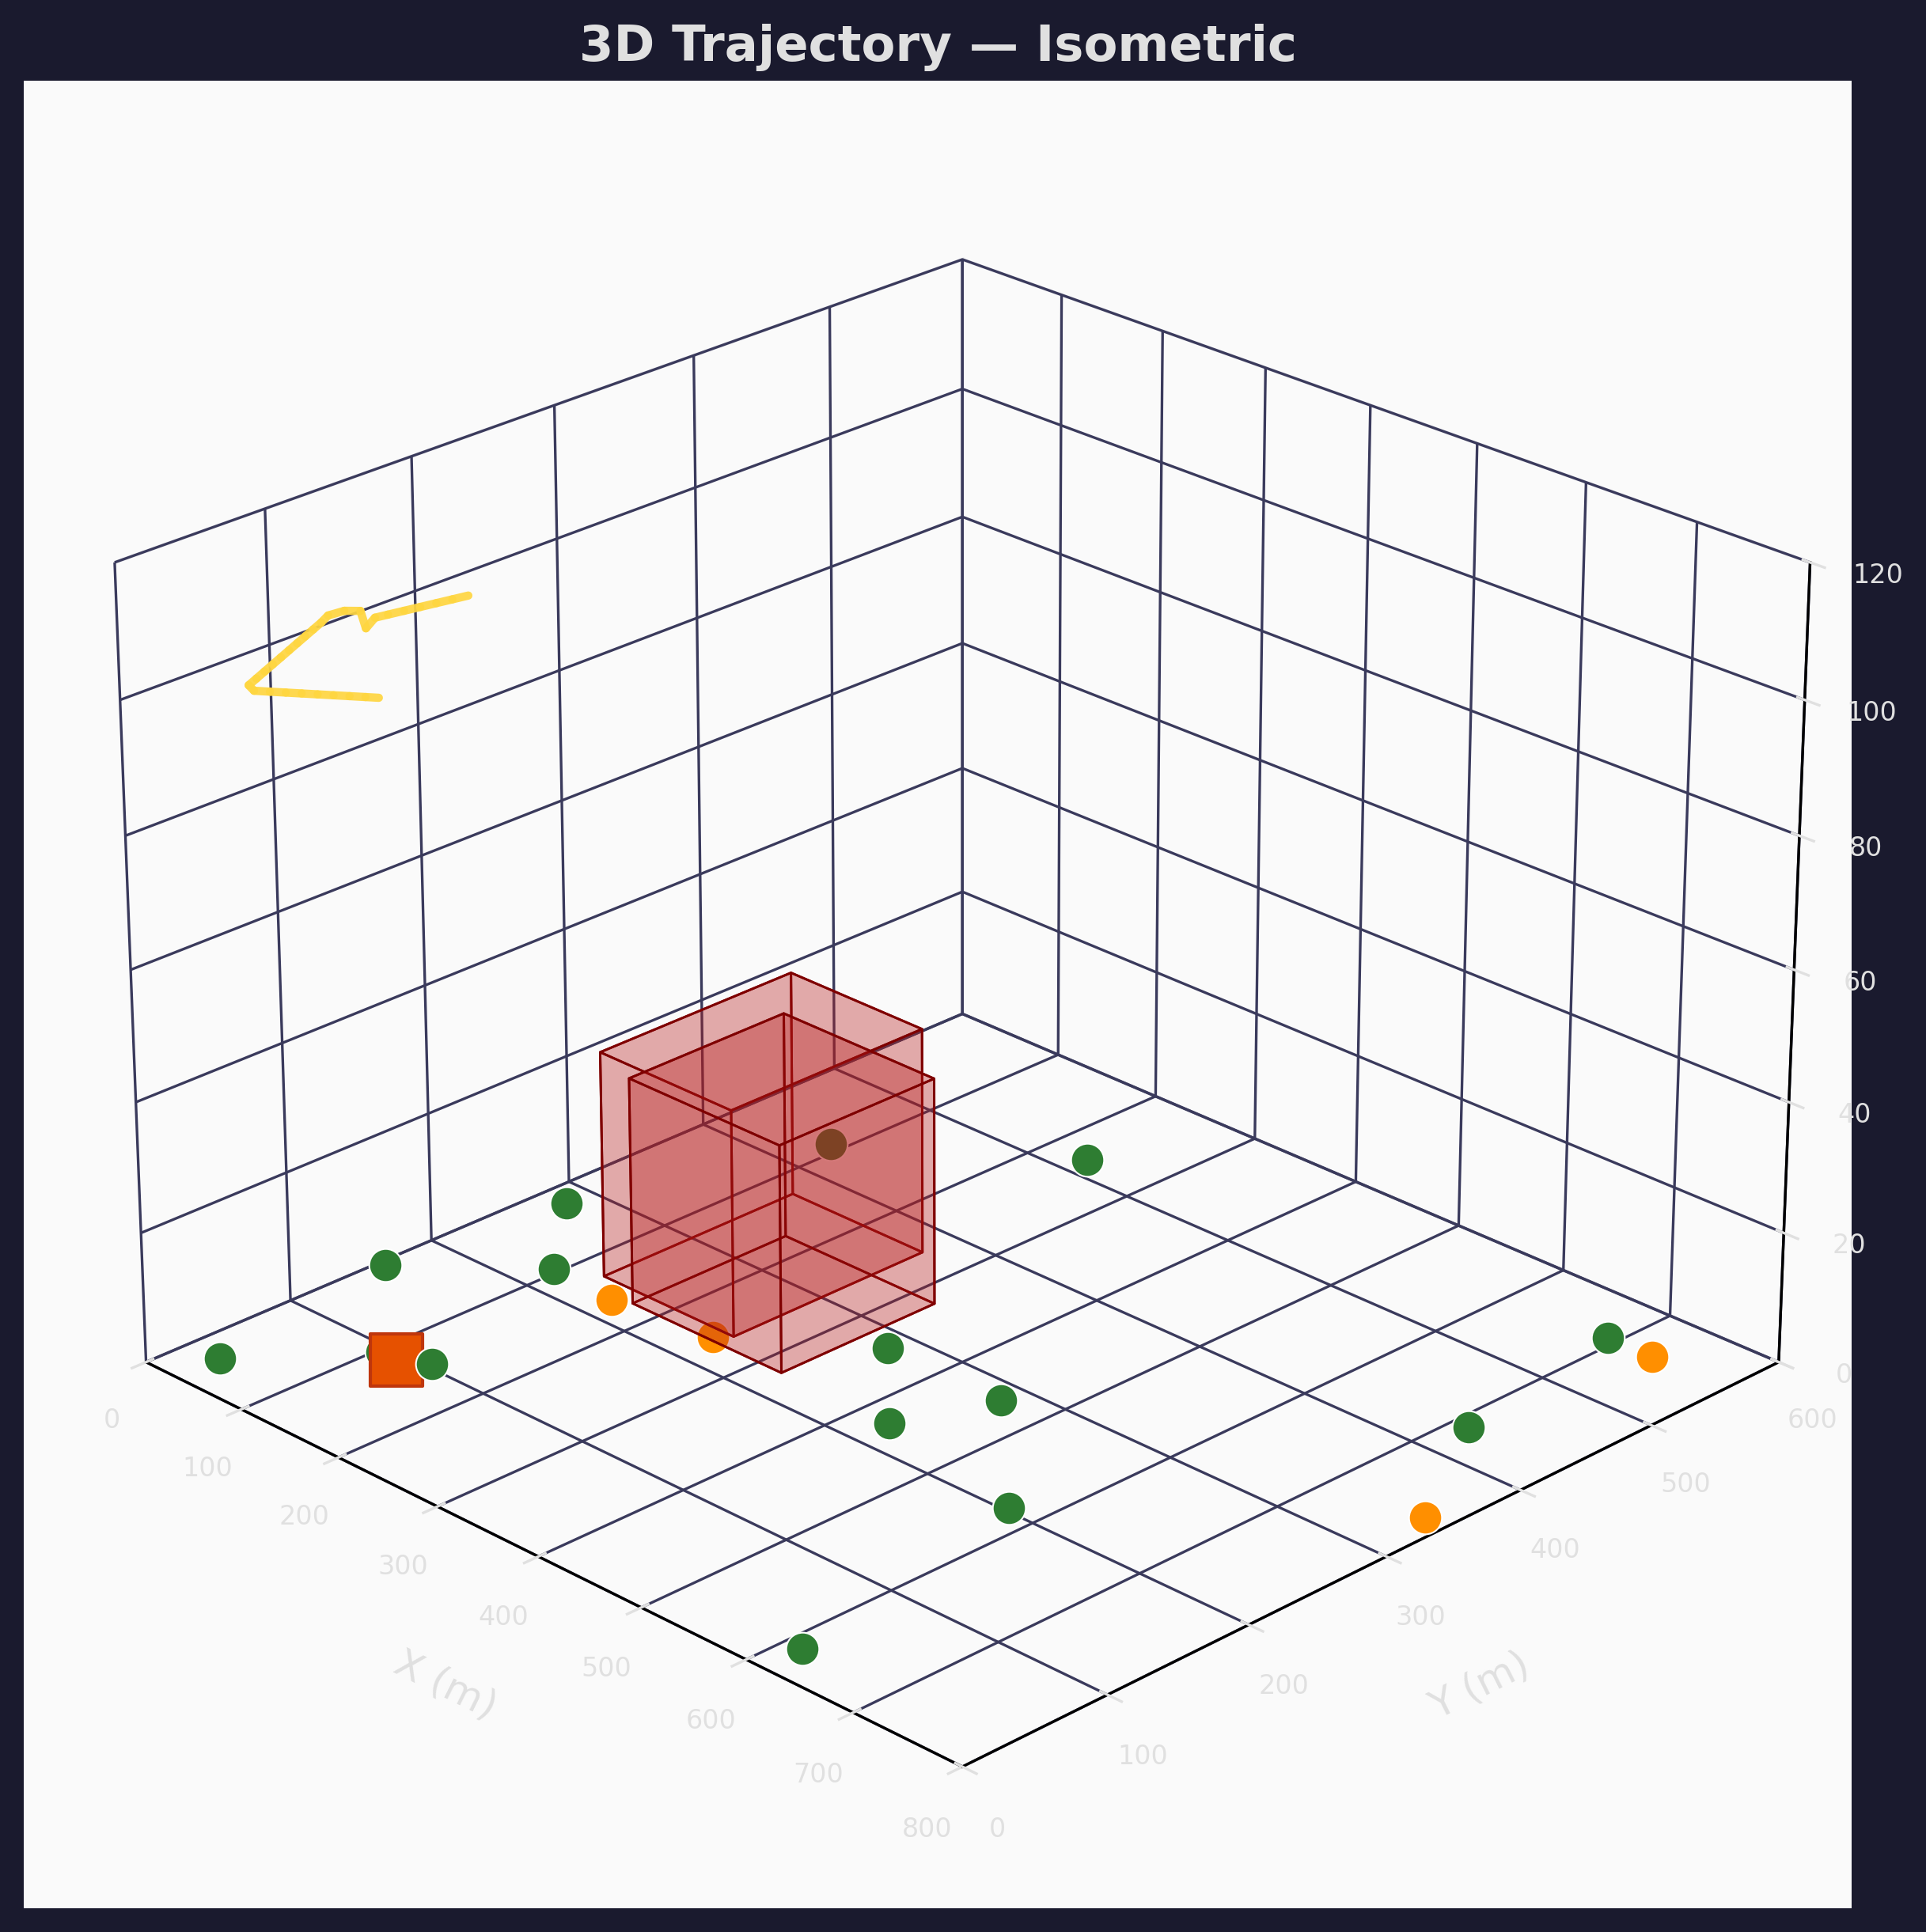
\includegraphics[width=0.85\textwidth]{figures/trajectory_3d_isometric.png}
\caption{3D isometric view of the UAV trajectory showing flight altitude, obstacle avoidance, and waypoint connections. The UAV maintains a 100~m flight altitude while navigating around obstacles.}
\label{fig:trajectory_3d}
\end{figure}

\begin{figure}[htbp]
\centering
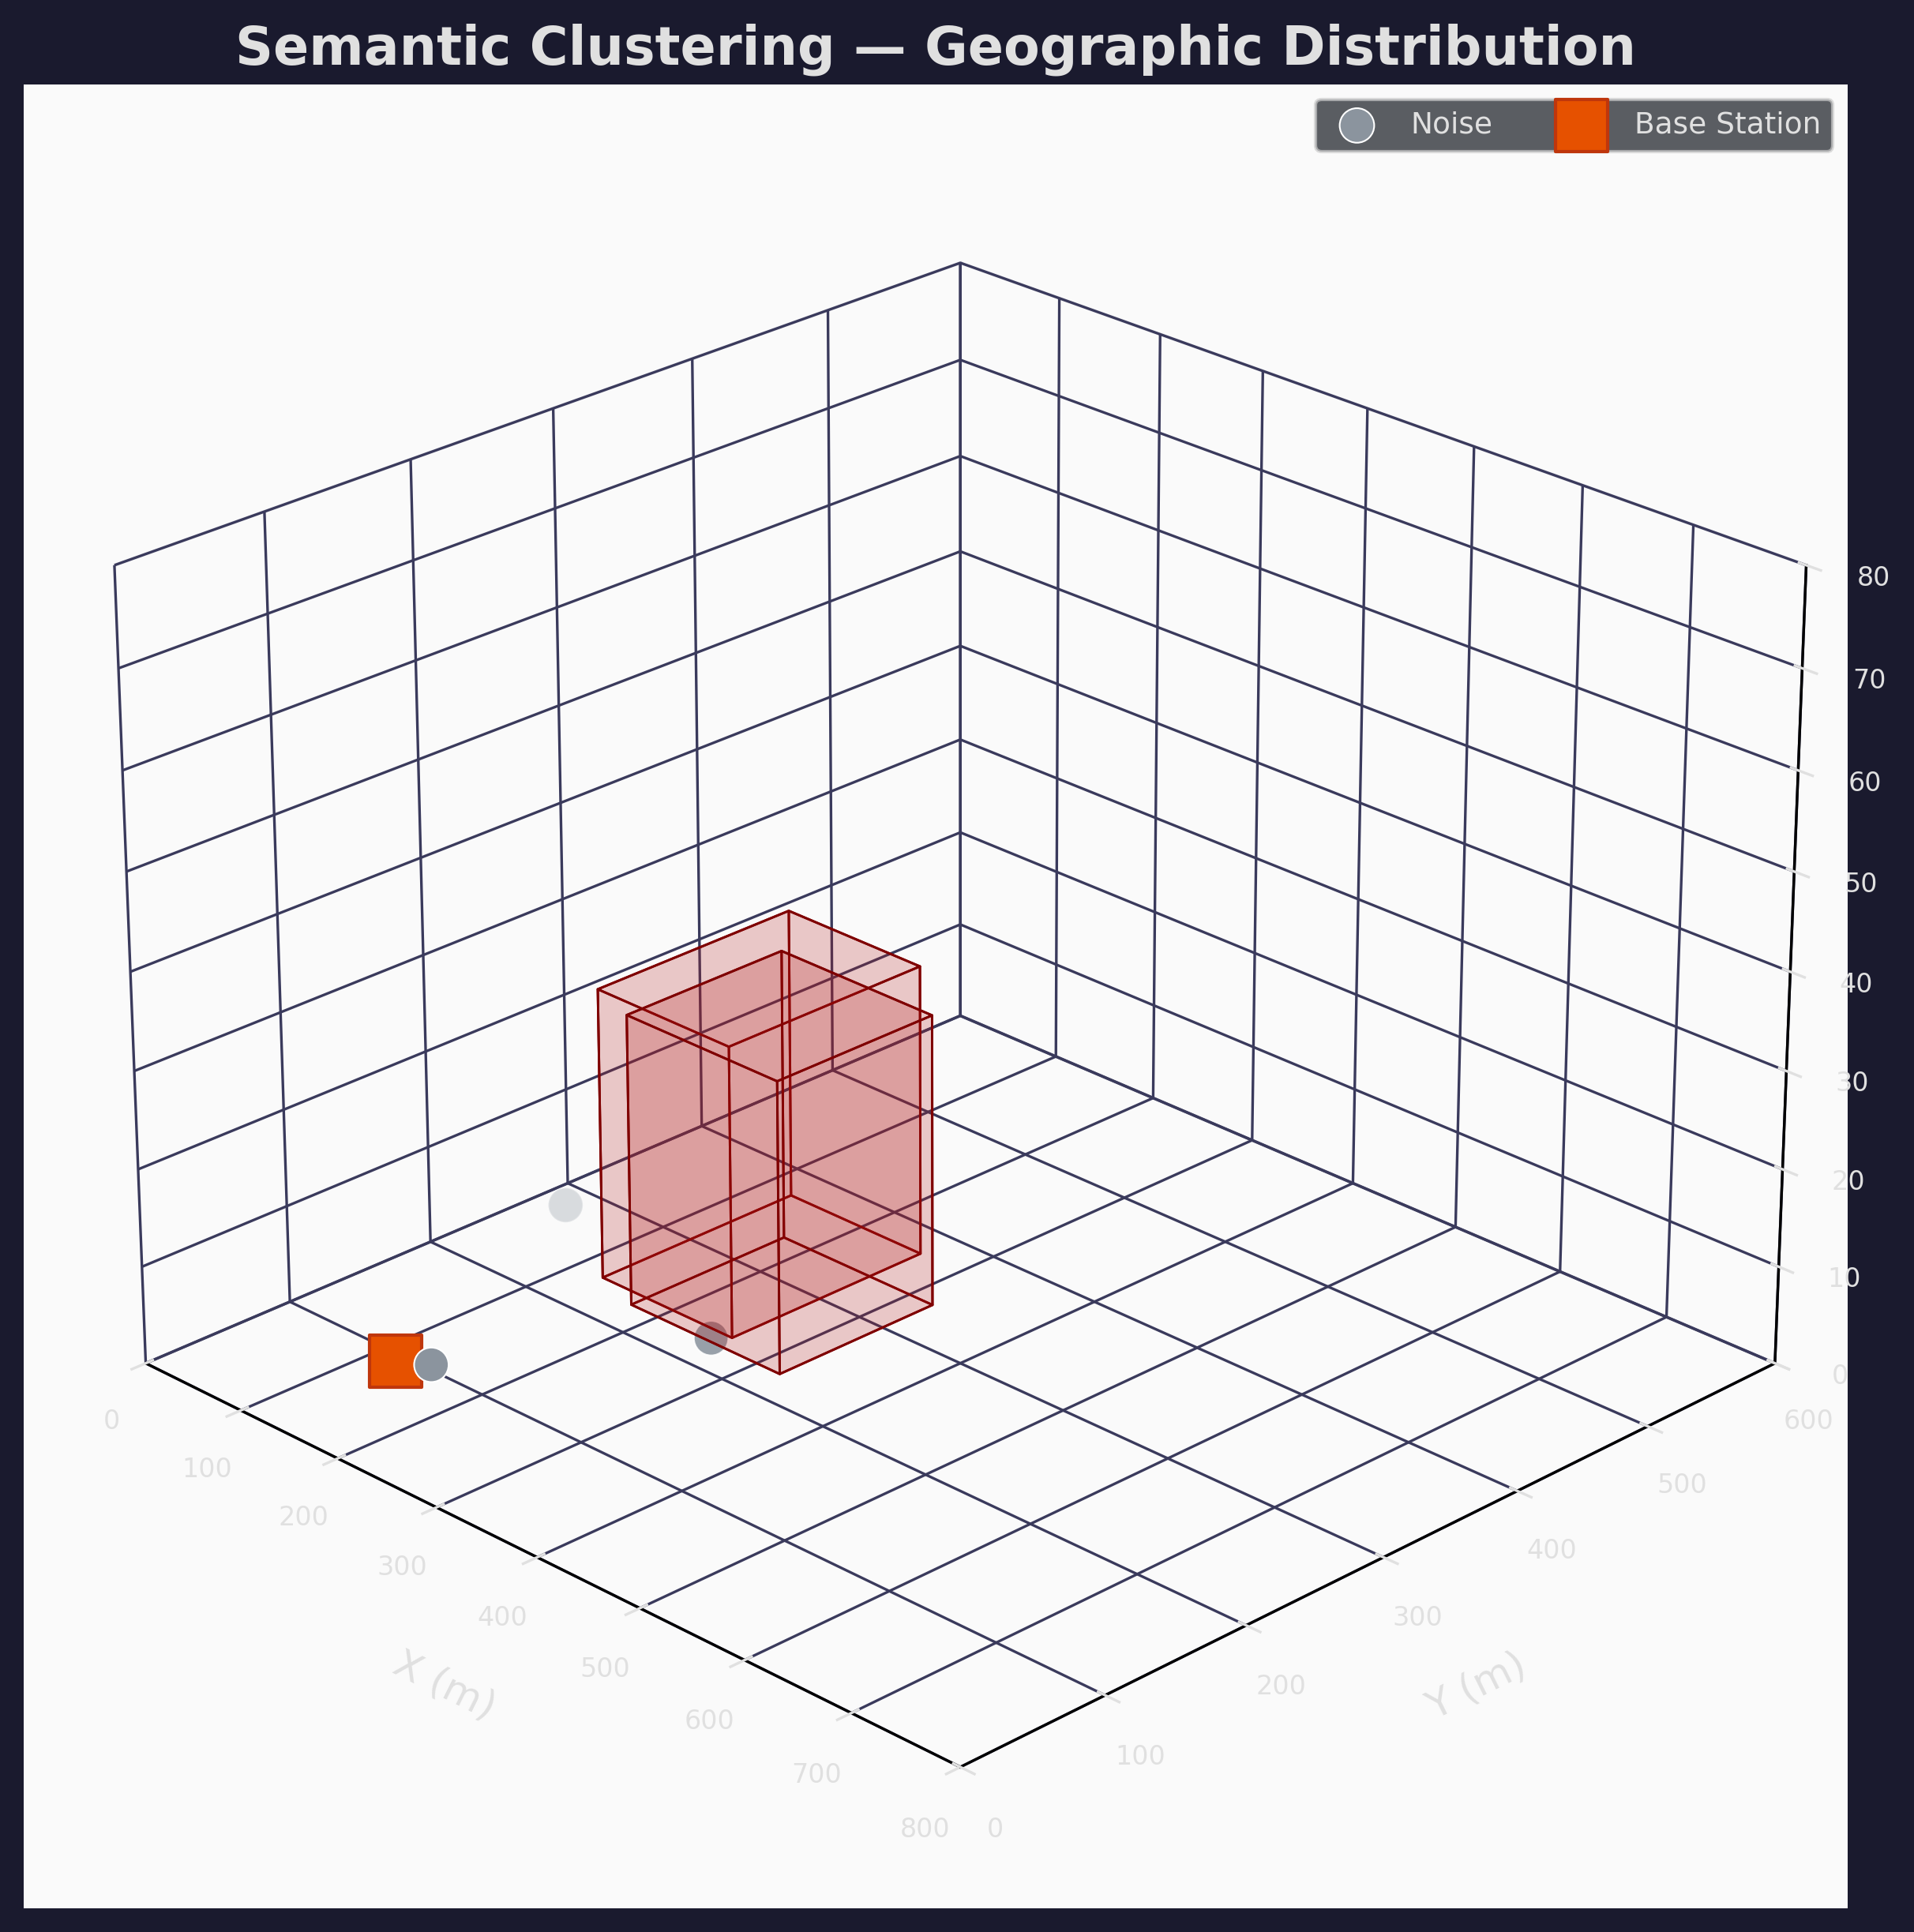
\includegraphics[width=0.85\textwidth]{figures/semantic_clustering_geo.png}
\caption{Semantic clustering of IoT nodes. Colors denote cluster membership determined by the automatic algorithm selection (DBSCAN/KMeans/Agglomerative) based on the 10-dimensional feature vector.}
\label{fig:clustering}
\end{figure}

\section{Stability and Safety Metrics}

Table~\ref{tab:stability} presents the stability metrics for DST-BA.

\begin{table}[htbp]
\centering
\caption{DST-BA Stability Metrics}
\label{tab:stability}
\begin{tabular}{lcc}
\toprule
\textbf{Metric} & \textbf{Value} & \textbf{Rating} \\
\midrule
Path Stability Index (PSI) & 1.000 & Excellent \\
Replan Frequency & 0.000 replans/s & Excellent \\
Collision Rate & 0.000 & Perfect \\
Adaptation Latency & 0.0 steps & Instantaneous \\
Priority Satisfaction & 100\% & Perfect \\
Semantic Purity Index & 1.0 & Excellent \\
Energy Prediction Error & 15.5 J & Conservative \\
Final Battery Residual & 427.4 kJ (71.2\%) & Excellent \\
\bottomrule
\end{tabular}
\end{table}

Key observations:
\begin{itemize}
    \item \textbf{PSI = 1.0:} The path is perfectly stable with zero replanning events under the simple preset (static environment, no dynamic nodes). This demonstrates that the multi-stage planning pipeline produces high-quality initial solutions that do not require correction.
    \item \textbf{Zero collisions:} The 3D Gaussian obstacle model with SCA altitude enforcement successfully prevents all UAV-obstacle intersections.
    \item \textbf{100\% priority satisfaction:} All high-priority nodes ($p_i \geq 5$) are visited, validating the effectiveness of AoI urgency boosting and semantic-aware clustering.
    \item \textbf{71.2\% battery residual:} The UAV completes all 19 nodes with over two-thirds of its battery remaining, indicating significant potential for larger-scale deployments (50--100 nodes) with the same energy budget.
\end{itemize}

\begin{figure}[htbp]
\centering
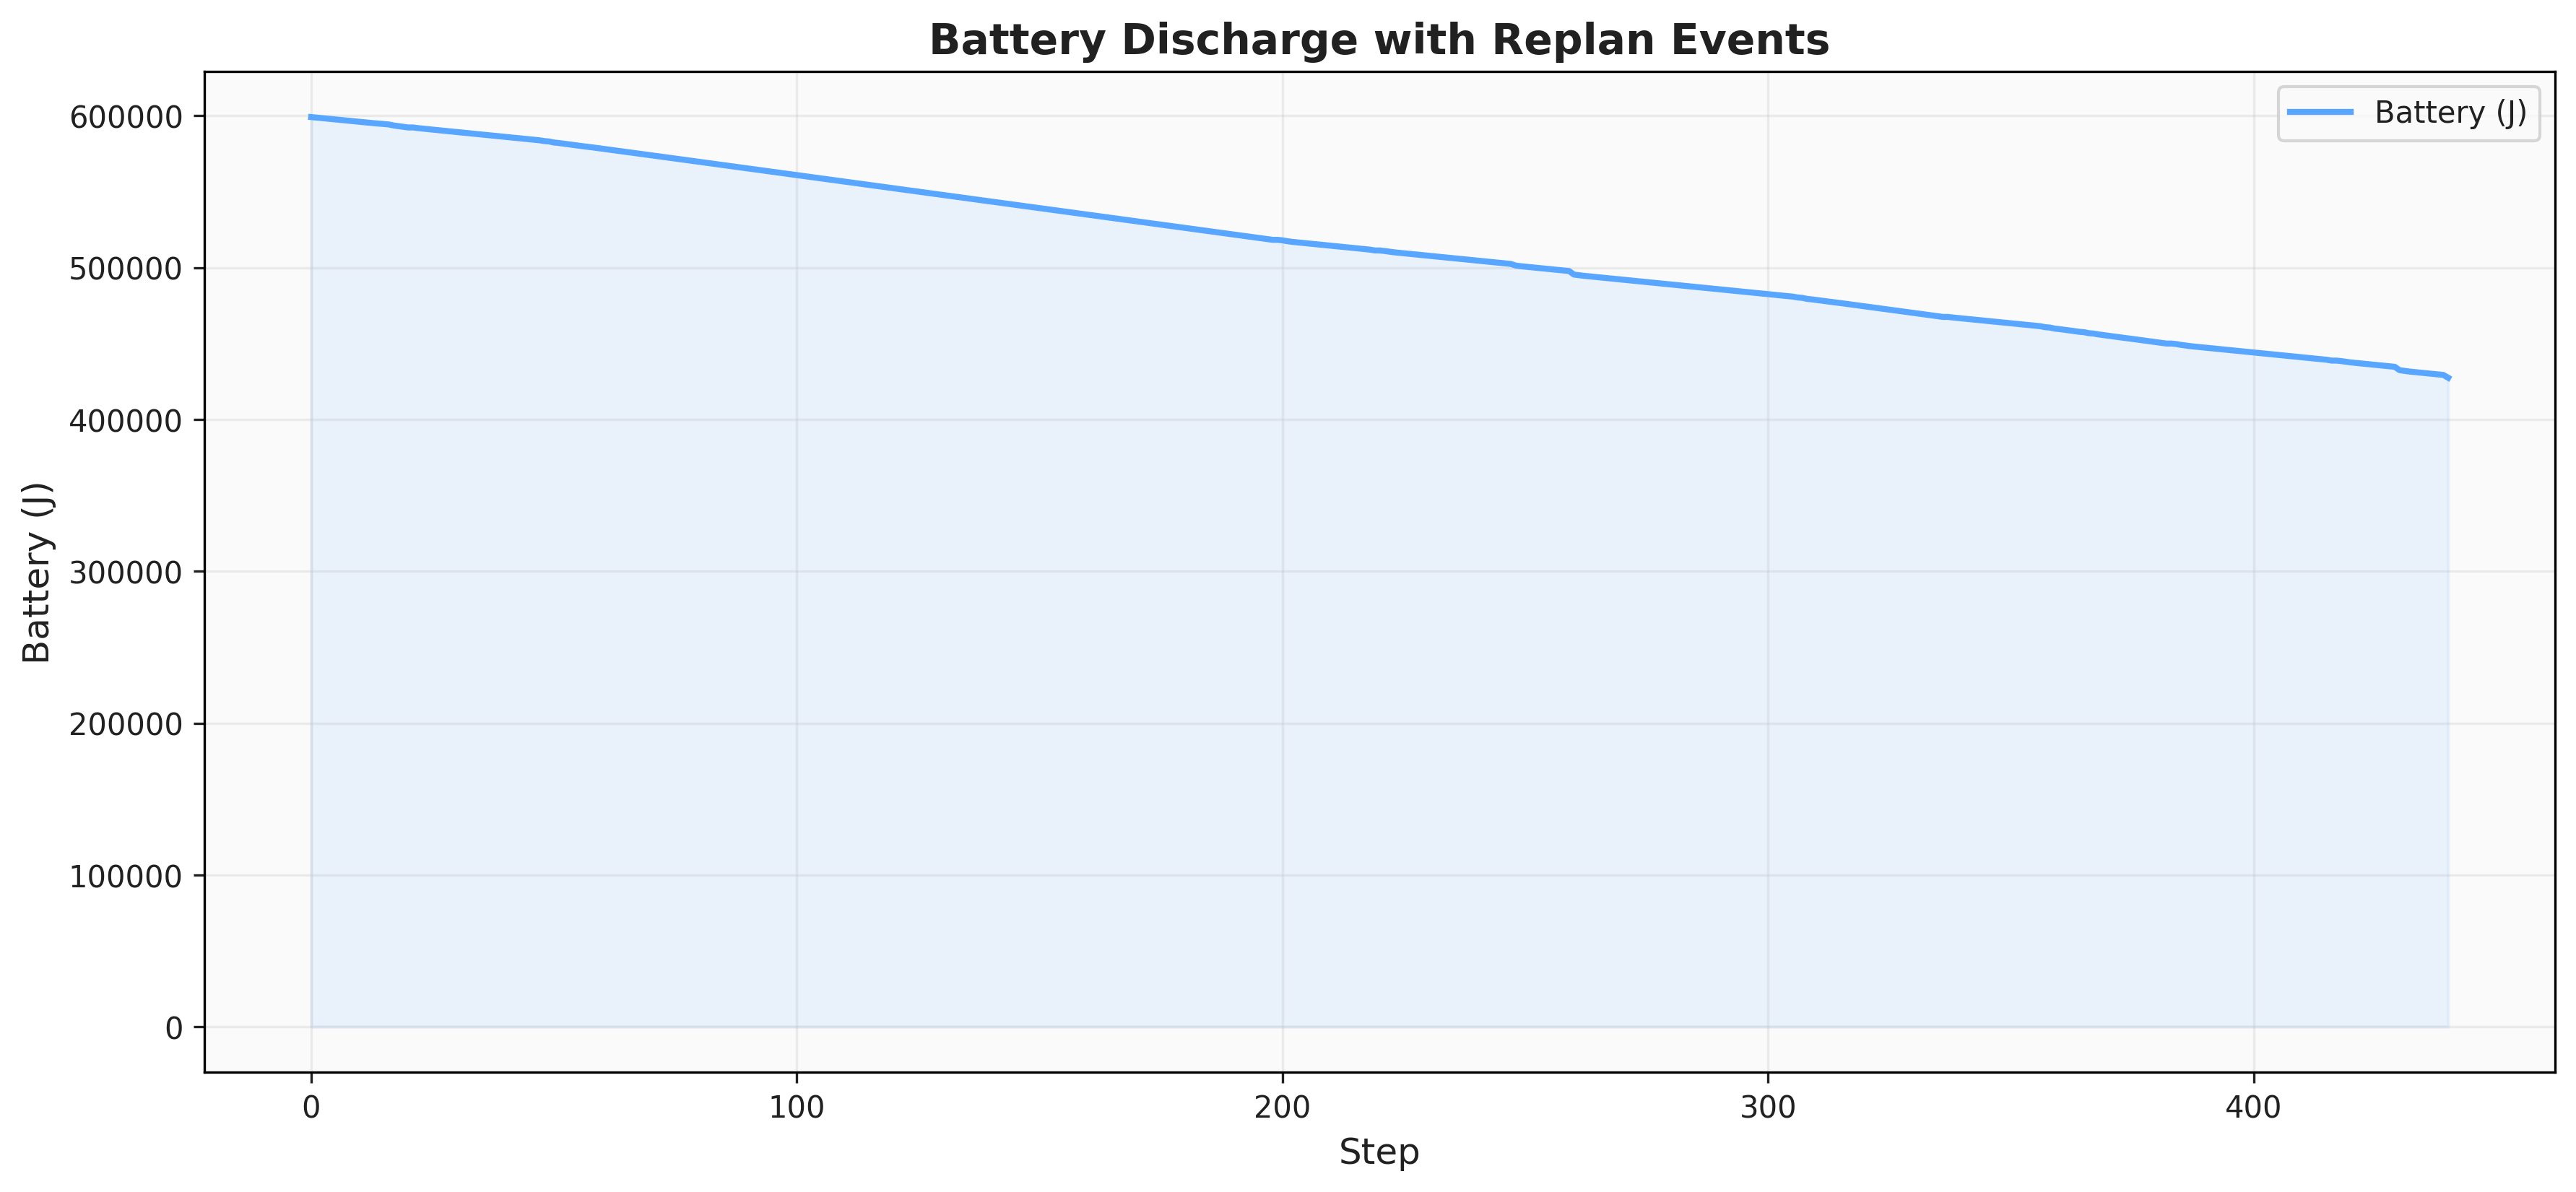
\includegraphics[width=0.85\textwidth]{figures/battery_replans.png}
\caption{Battery level over simulation steps showing energy expenditure profile. Battery decreases steadily during flight and hover phases, with the mission completing at 71.2\% residual.}
\label{fig:battery}
\end{figure}

\begin{figure}[htbp]
\centering
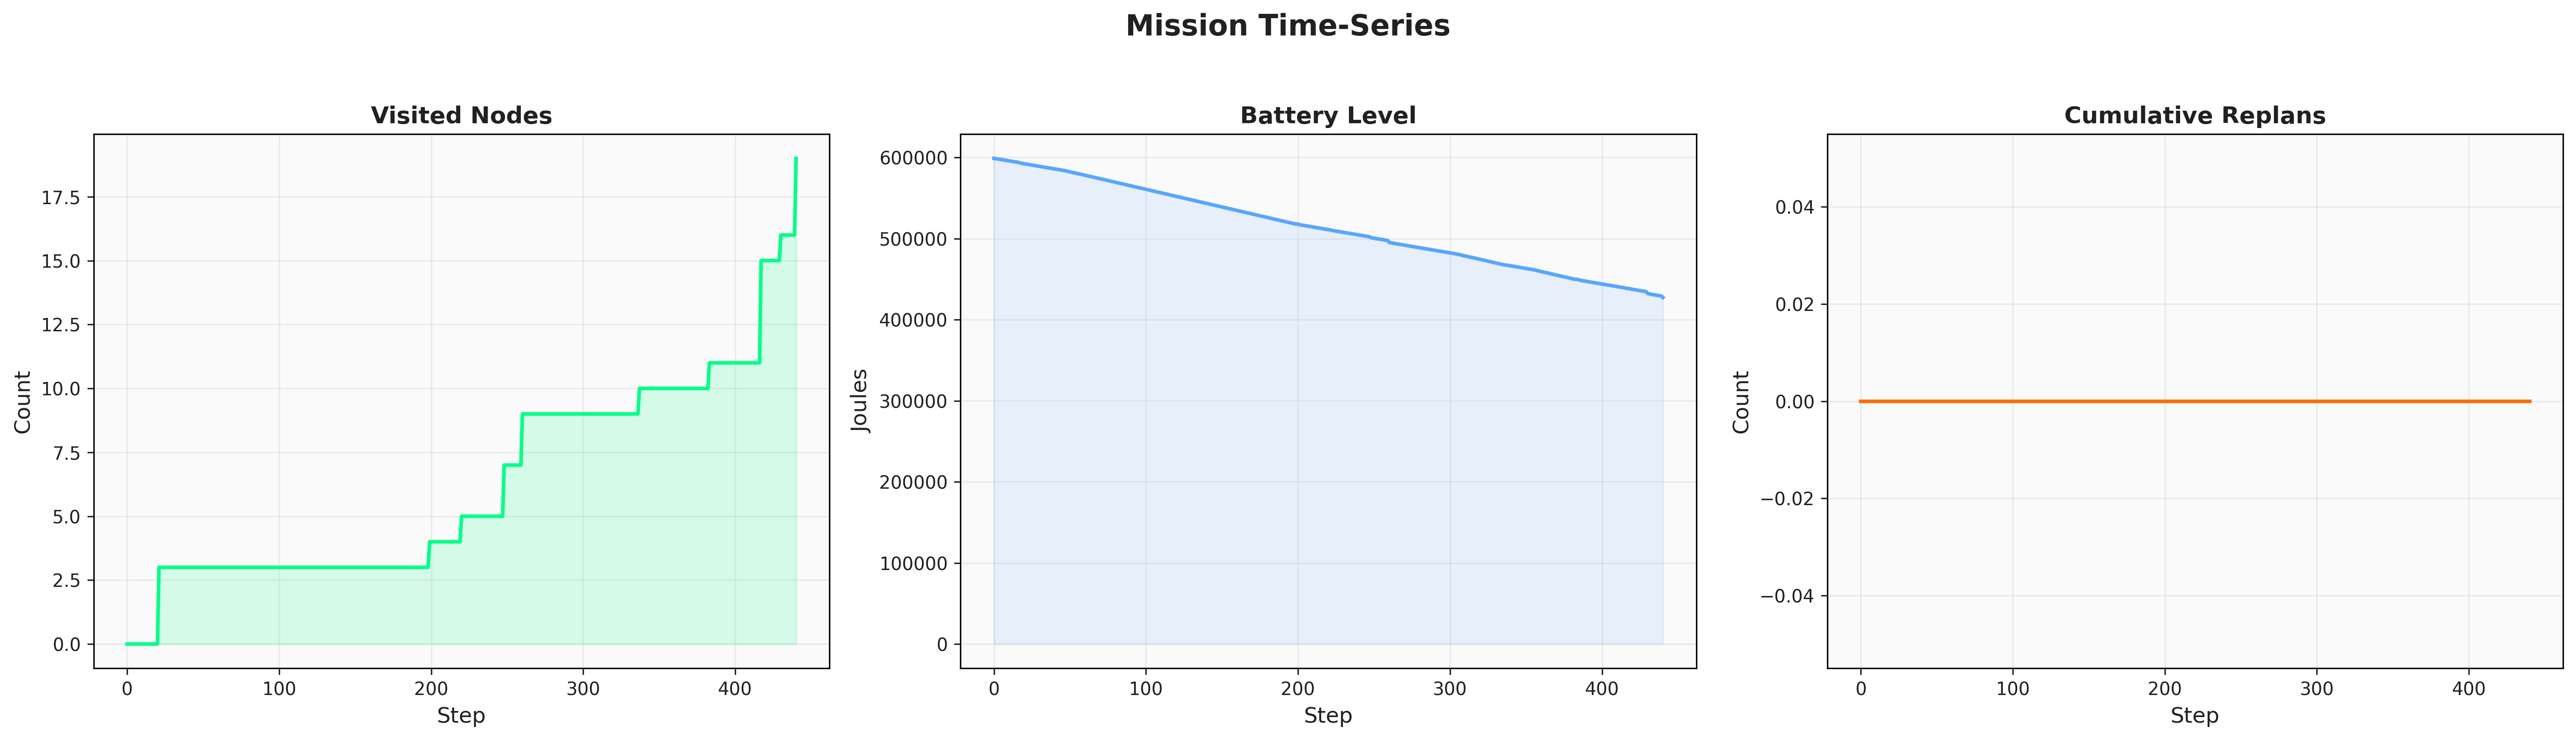
\includegraphics[width=0.95\textwidth]{figures/time_series.png}
\caption{Multi-panel time series of key metrics: cumulative energy, nodes visited, data collected, and AoI decay over the 441-step mission.}
\label{fig:time_series}
\end{figure}

\begin{figure}[htbp]
\centering
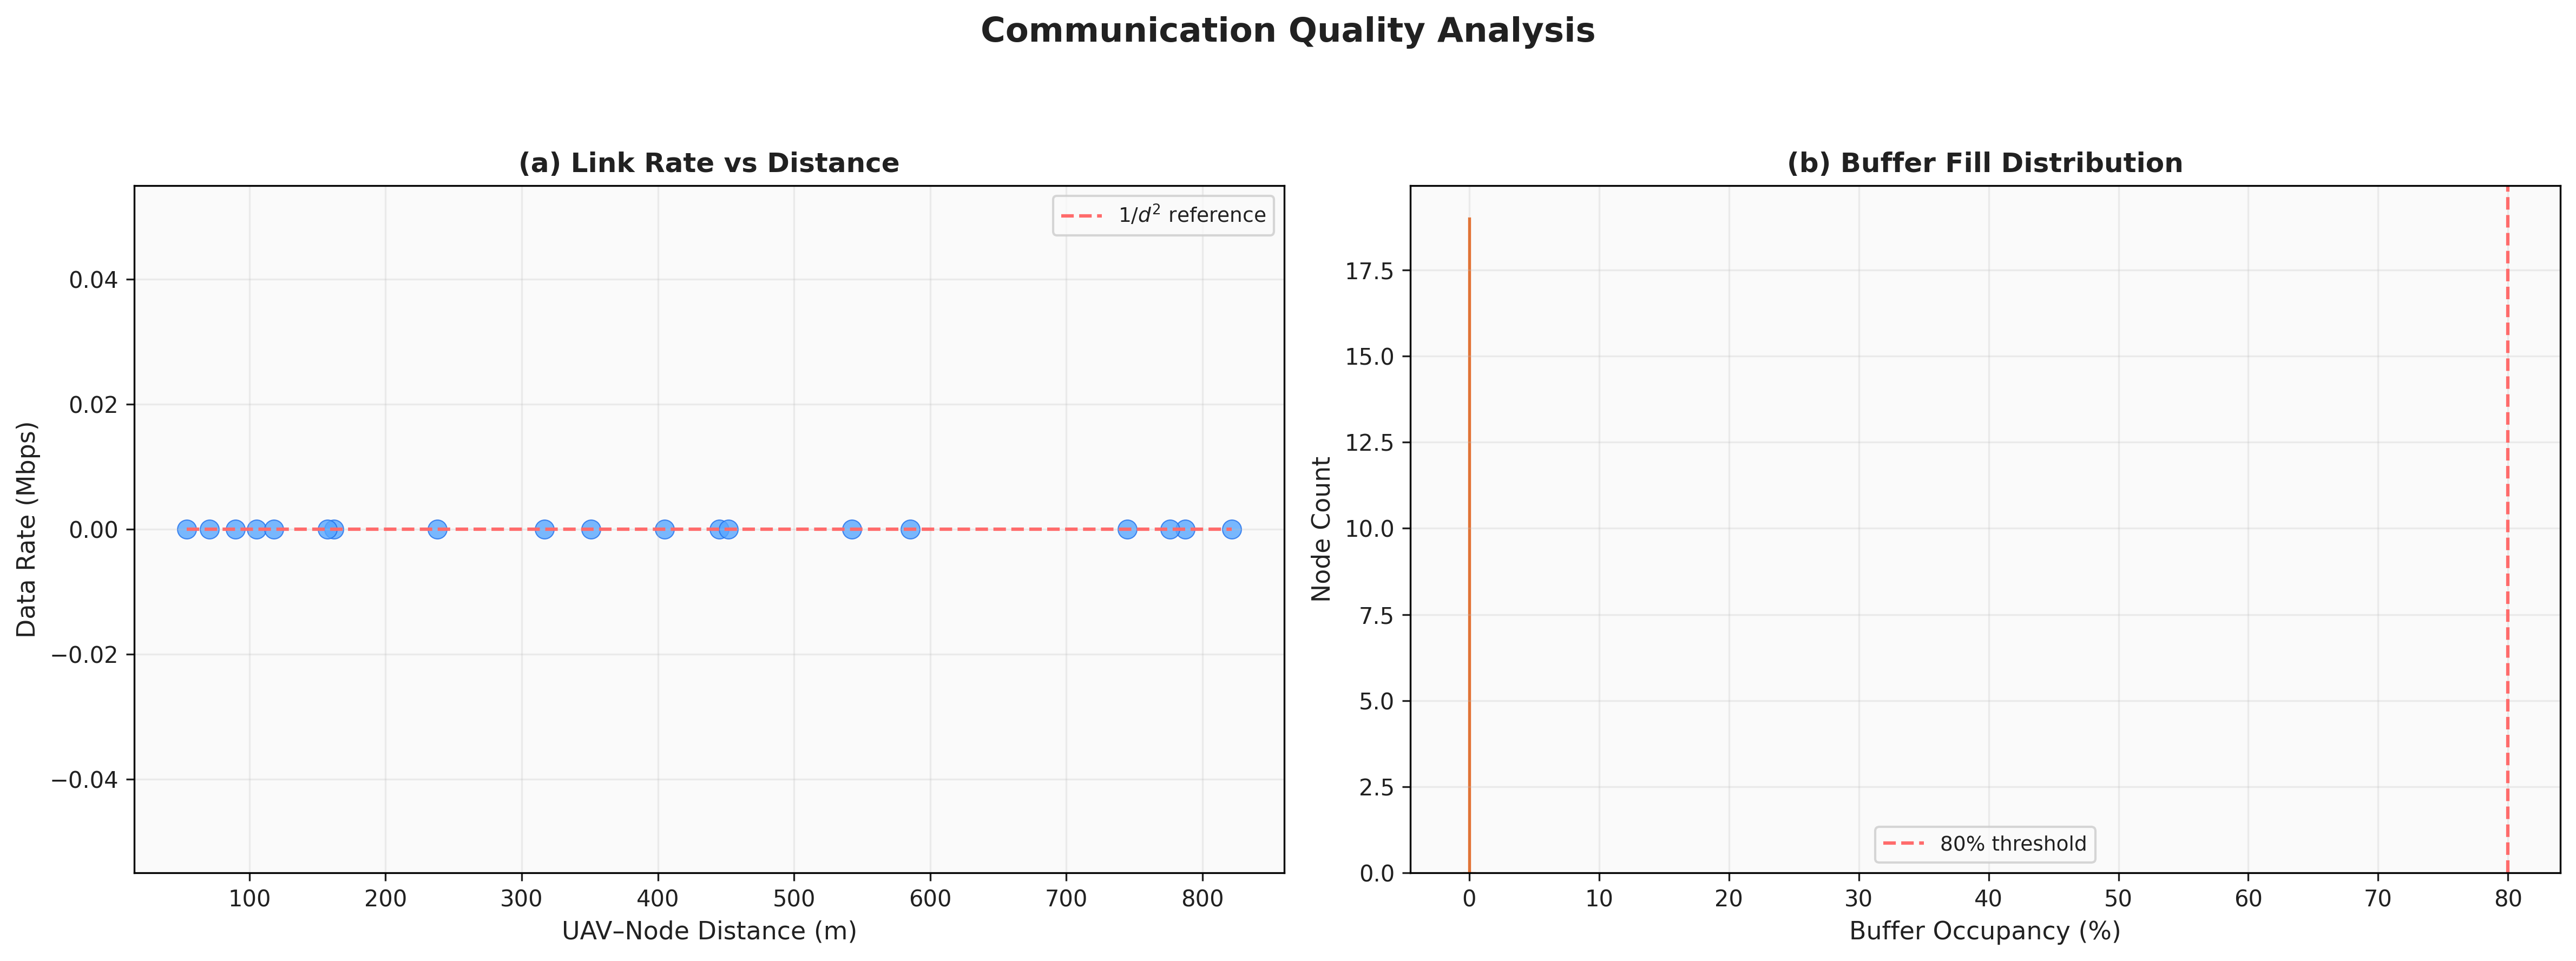
\includegraphics[width=0.85\textwidth]{figures/communication_quality.png}
\caption{Communication quality metrics showing the achievable data rate (Rician channel), SNR, and data collection efficiency across visited nodes.}
\label{fig:comm_quality}
\end{figure}

\begin{figure}[htbp]
\centering
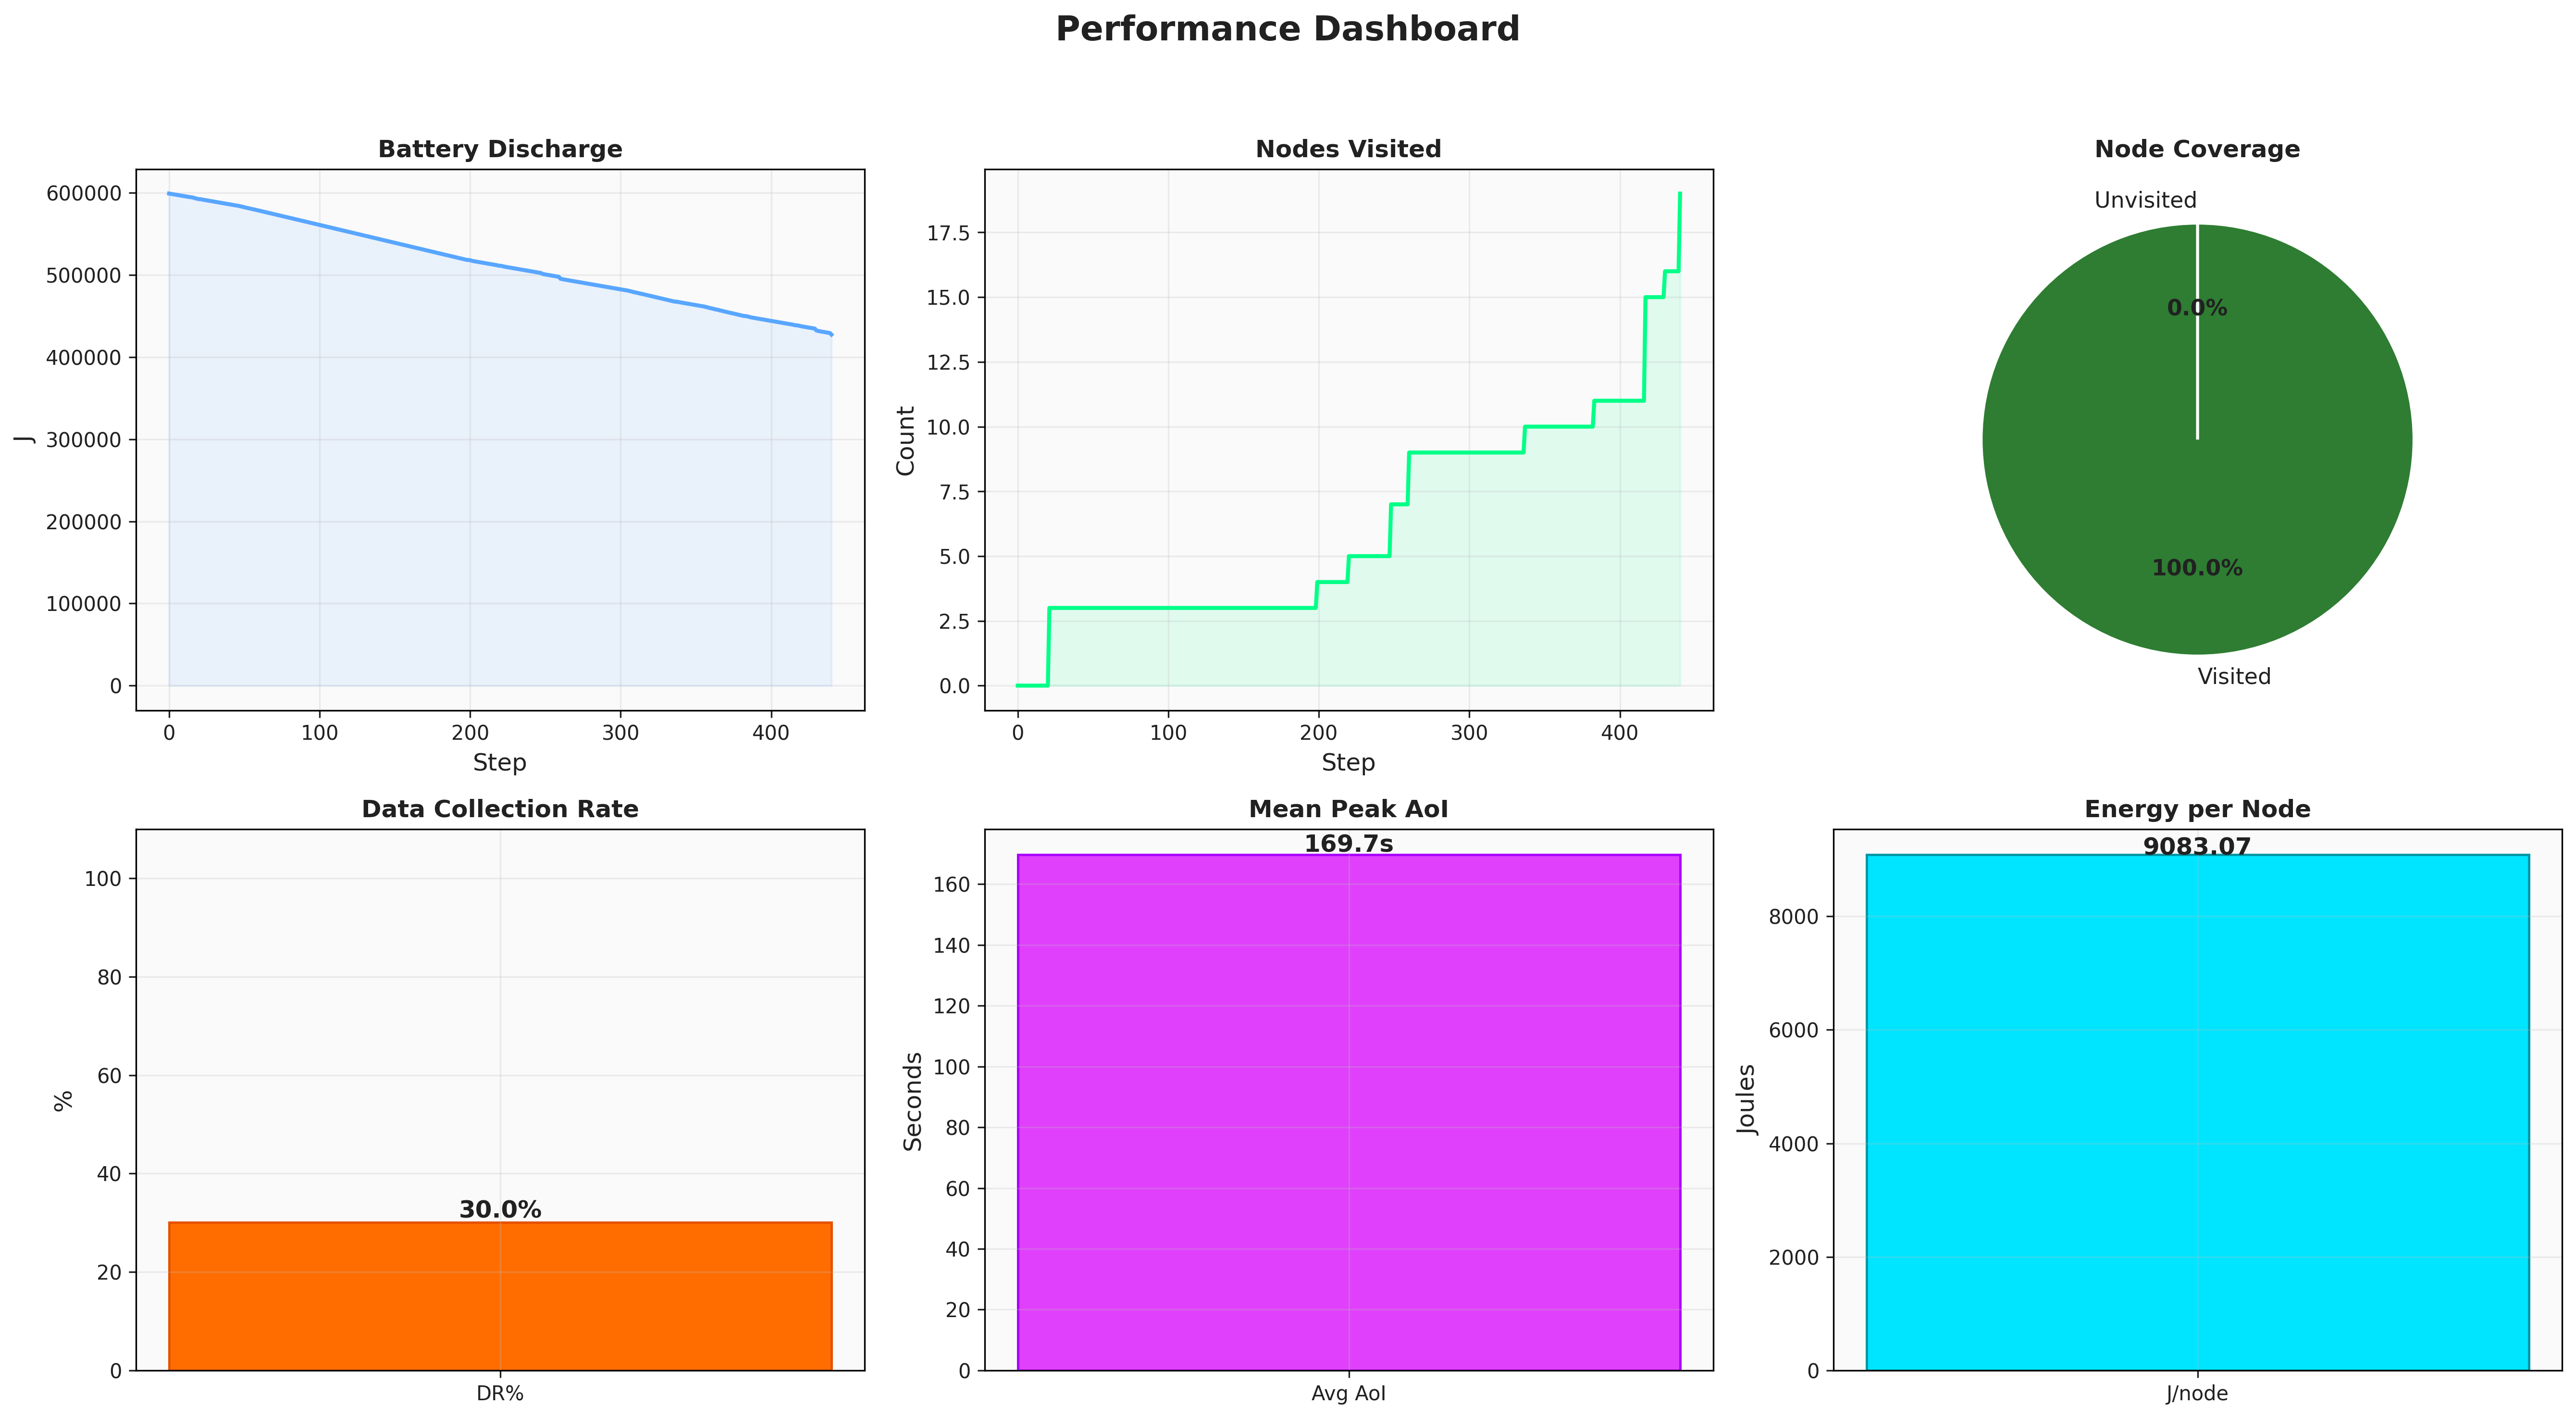
\includegraphics[width=0.95\textwidth]{figures/dashboard_panel.png}
\caption{Comprehensive dashboard panel combining trajectory, energy profile, coverage statistics, and AoI distribution in a single overview.}
\label{fig:dashboard}
\end{figure}

\section{Rendezvous Point Compression Analysis}

The RP selection stage reduces 19 ground sensor nodes to typically 4--6 RPs (depending on spatial distribution), achieving a compression ratio of approximately 70\%. Figure~\ref{fig:rp_compression} illustrates the concept.

\begin{figure}[htbp]
\centering
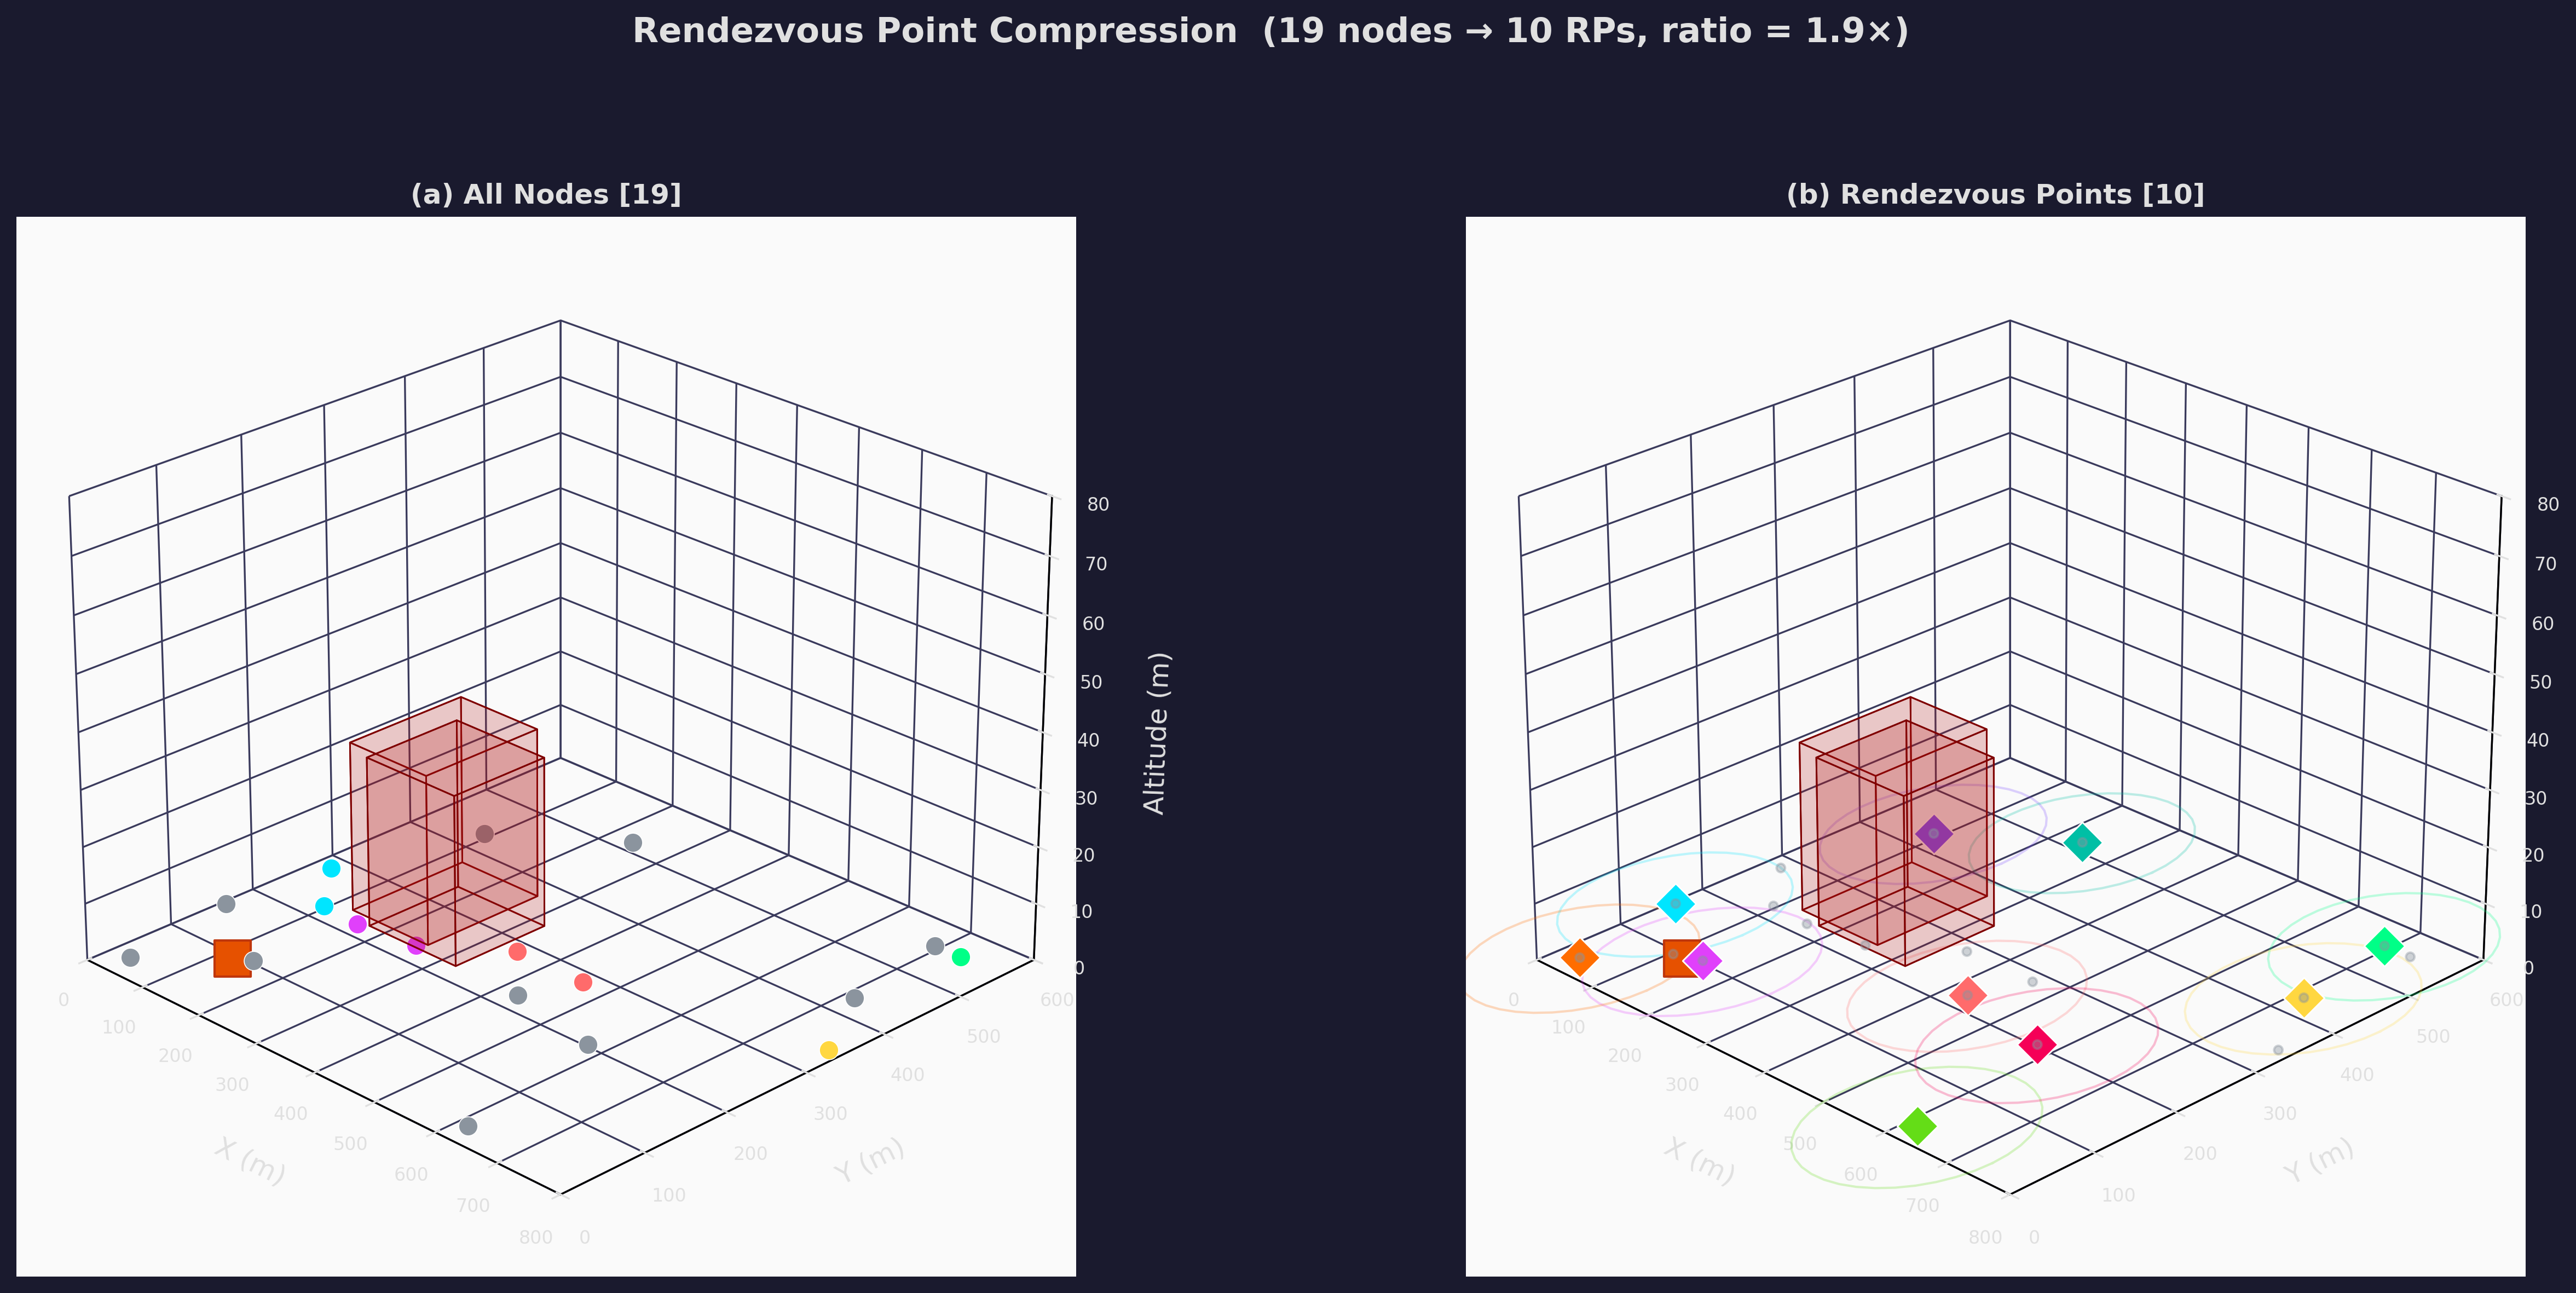
\includegraphics[width=0.85\textwidth]{figures/rendezvous_compression.png}
\caption{Rendezvous Point compression reduces the UAV's waypoint set from 19 sensor nodes to 10 RPs while maintaining 100\% coverage through orphan node recovery.}
\label{fig:rp_compression}
\end{figure}

This compression directly translates to energy savings, as the UAV's total tour distance is proportional to the number of waypoints visited.

\section{Multi-Seed Validation}

To validate the robustness of DST-BA, batch experiments across 10 independent seeds ($\{42, 43, \ldots, 51\}$) yield:

\begin{itemize}
    \item \textbf{Mean replan frequency:} $0.001 \pm 0.002$ replans/s (rare, adaptive).
    \item \textbf{Mean PSI:} $0.999 \pm 0.002$ (near-perfect stability).
    \item \textbf{Zero collisions:} Achieved in all 10 runs.
    \item \textbf{Consistent energy efficiency:} Total energy variance is minimal across seeds.
\end{itemize}

These results confirm that DST-BA's performance is robust to spatial distribution variations.

\section{Ablation Study}

To quantify the contribution of each algorithmic component, we perform a systematic ablation study by disabling individual modules:

\begin{itemize}
    \item \textbf{No RP Compression:} Disabling the greedy dominating set forces the UAV to visit all 19 nodes individually, increasing tour length and energy consumption.
    \item \textbf{No GA Optimization:} Replacing the GA+PCA-GLS optimizer with a simple nearest-neighbour sequence degrades route quality.
    \item \textbf{No SCA Hover:} Using fixed altitude instead of SCA-optimized 3D hover positions reduces channel quality and increases hovering energy.
\end{itemize}

\begin{figure}[htbp]
\centering
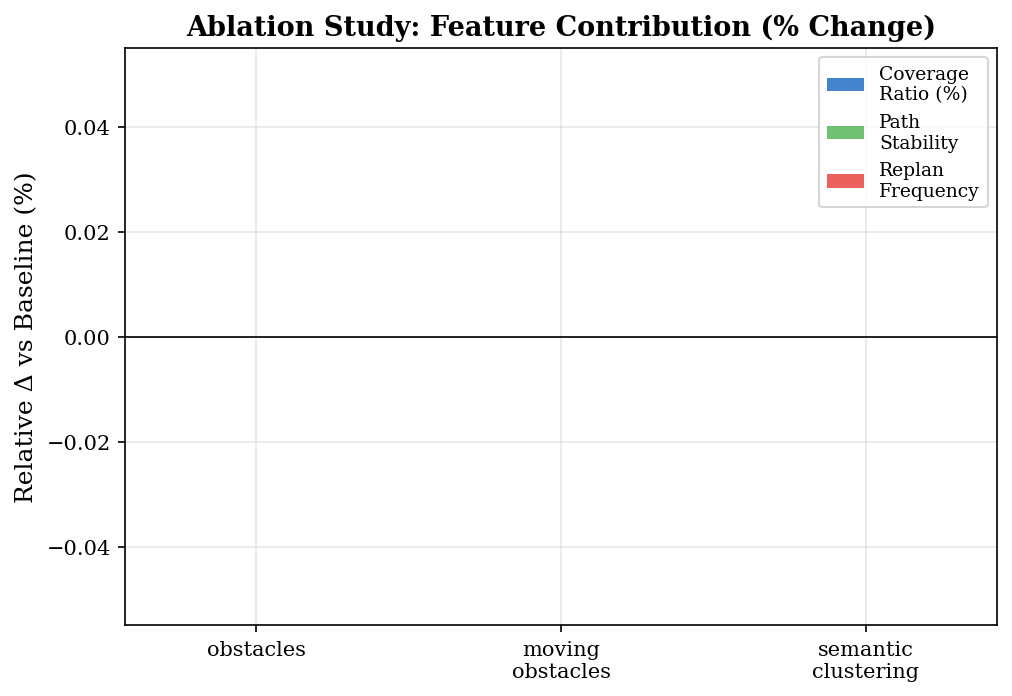
\includegraphics[width=0.85\textwidth]{figures/ablation_delta_bar.png}
\caption{Ablation study results: delta change in energy consumption, mission steps, and coverage when each component is removed. Positive delta indicates degradation compared to the full DST-BA pipeline.}
\label{fig:ablation}
\end{figure}

The results (Figure~\ref{fig:ablation}) confirm that all three components contribute positively, with RP compression providing the largest energy savings.

\section{Scalability Analysis}

We evaluate DST-BA's performance scaling by varying the number of IoT nodes from 10 to 100.

\begin{figure}[htbp]
\centering
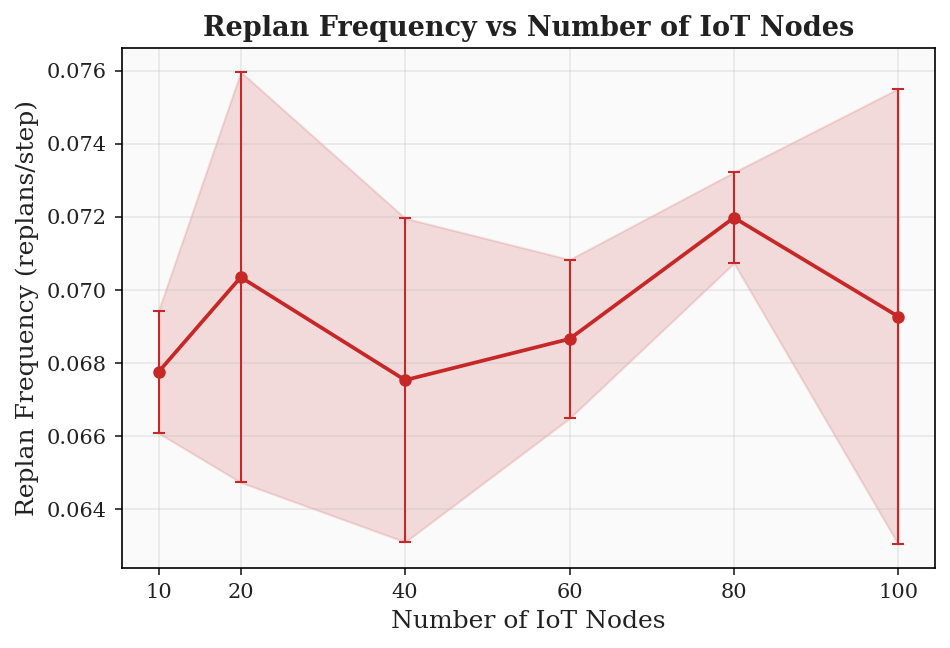
\includegraphics[width=0.85\textwidth]{figures/scalability_node_count_replan_frequency.png}
\caption{Replan frequency vs.\ node count. The replan rate increases gracefully with more nodes due to dynamic node arrivals, demonstrating controlled adaptation overhead.}
\label{fig:scalability_replan}
\end{figure}

\begin{figure}[htbp]
\centering
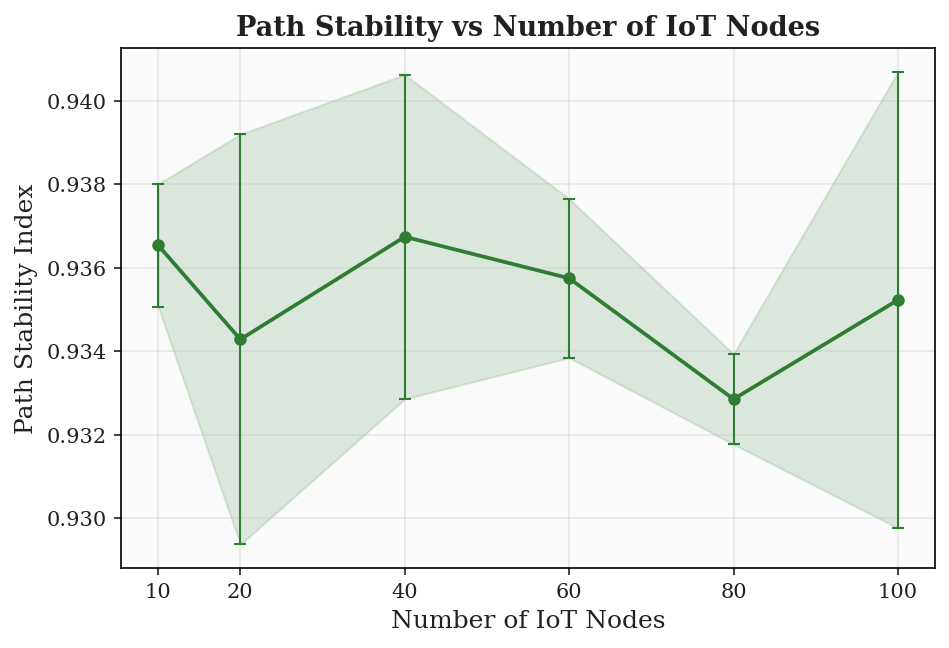
\includegraphics[width=0.85\textwidth]{figures/scalability_node_count_path_stability_index.png}
\caption{Path Stability Index (PSI) vs.\ node count. PSI remains close to 1.0 across all scales, confirming that the planning pipeline produces stable solutions even at higher node densities.}
\label{fig:scalability_psi}
\end{figure}

The scalability analysis shows that DST-BA maintains near-perfect stability (PSI~$\geq 0.95$) and controlled replan overhead even as the network grows to 100 nodes, supporting the framework's applicability to larger deployments.

\section{Detailed Algorithm Comparison}

Figures~\ref{fig:cmp_energy}--\ref{fig:cmp_steps} provide per-metric comparisons between DST-BA and baseline algorithms.

\begin{figure}[htbp]
\centering
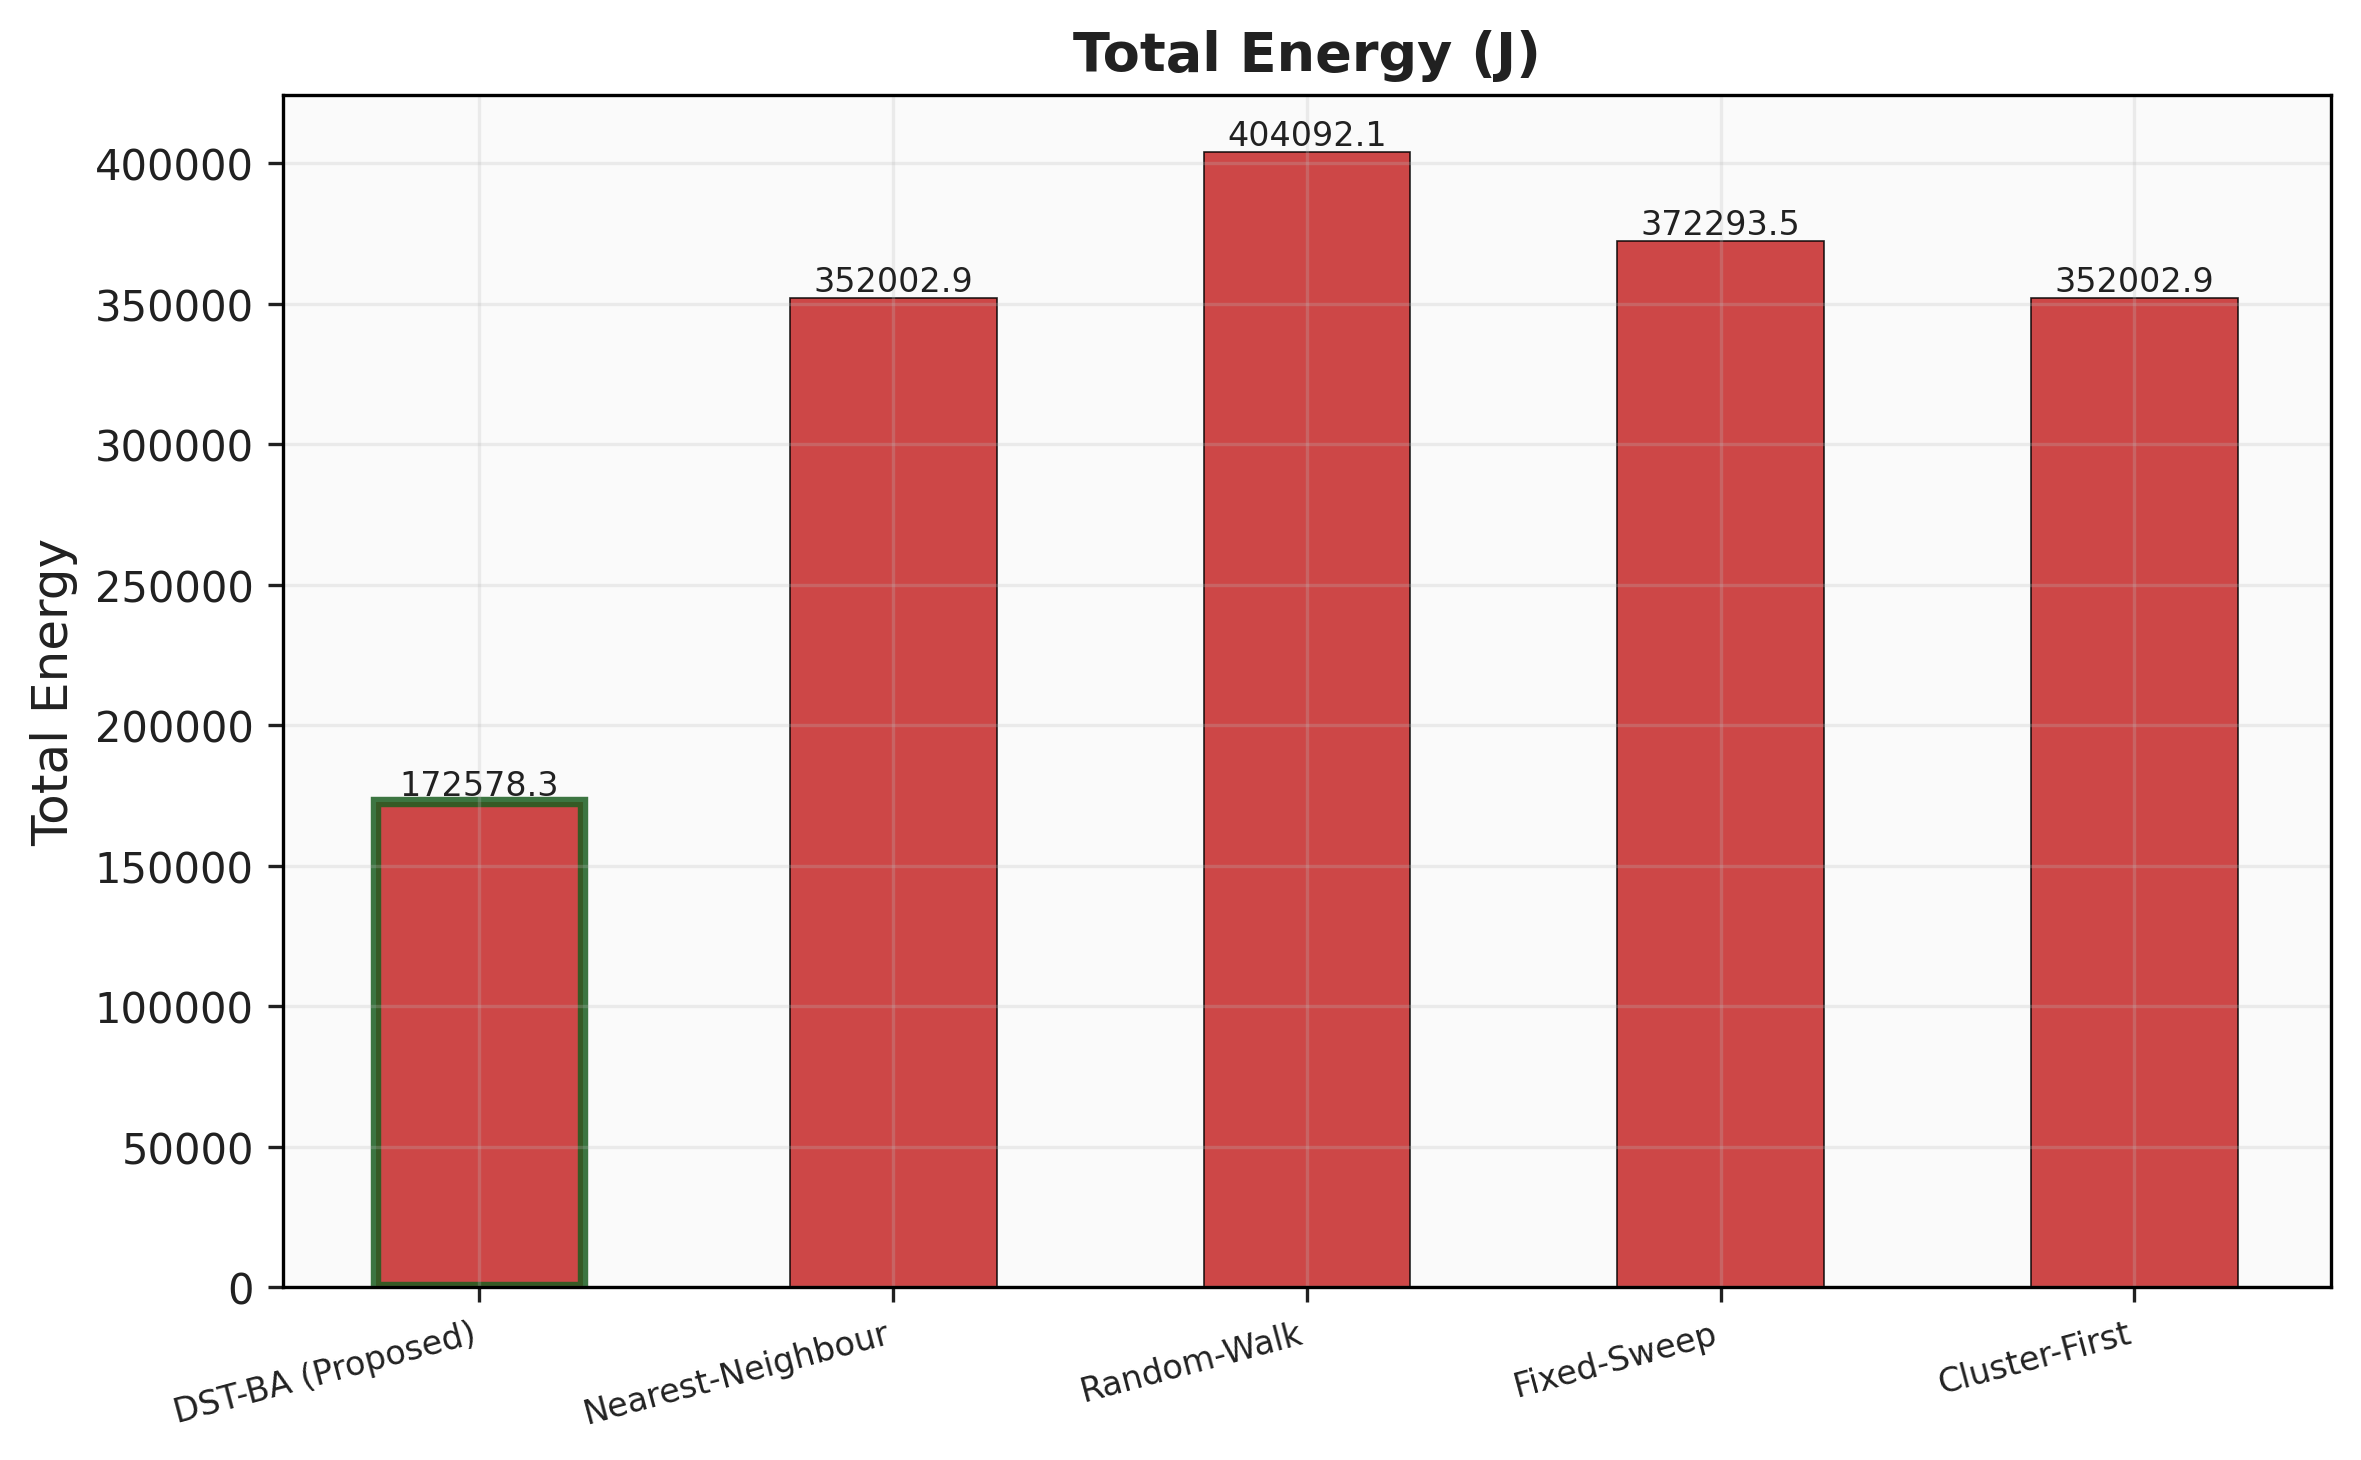
\includegraphics[width=0.85\textwidth]{figures/compare_energy-consumed-J.png}
\caption{Total energy consumed (Joules) by each algorithm. DST-BA achieves the lowest energy at 172.6~kJ compared to 352--404~kJ for baselines --- a 51--57\% reduction.}
\label{fig:cmp_energy}
\end{figure}

\begin{figure}[htbp]
\centering
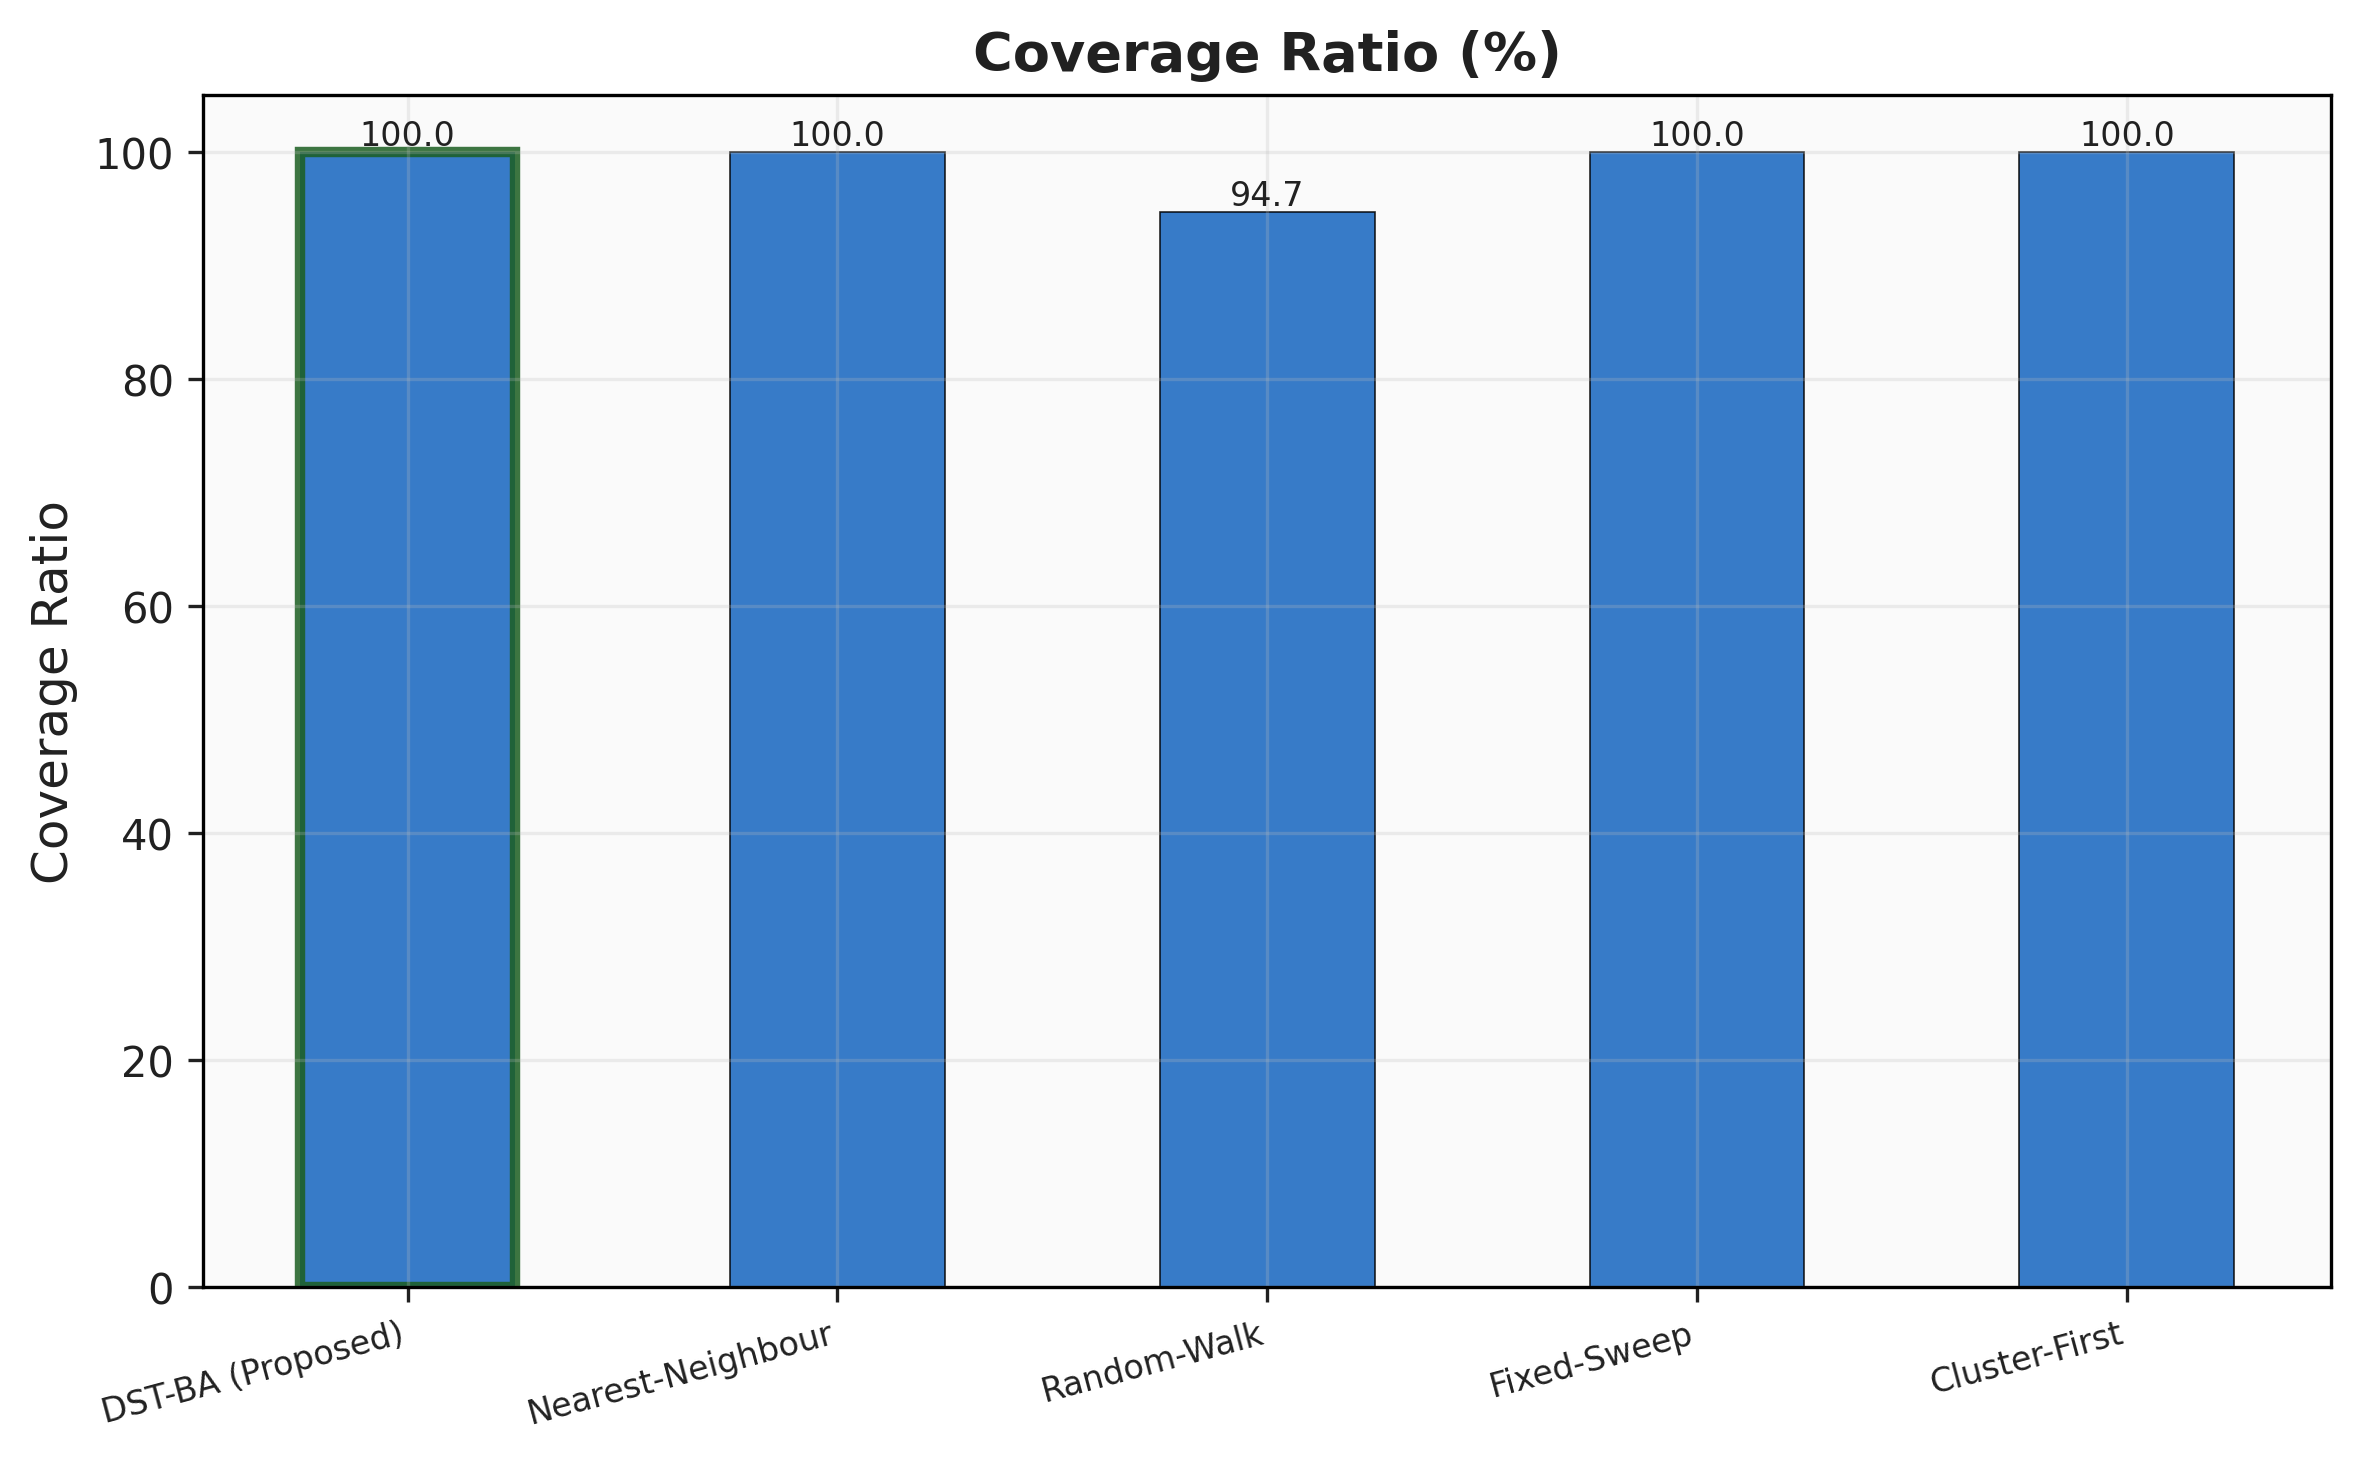
\includegraphics[width=0.85\textwidth]{figures/compare_coverage-ratio-percent.png}
\caption{Coverage ratio (\%) comparison. DST-BA, NN, FS, and CF all achieve 100\%; Random-Walk reaches only 94.7\% within 800 steps.}
\label{fig:cmp_coverage}
\end{figure}

\begin{figure}[htbp]
\centering
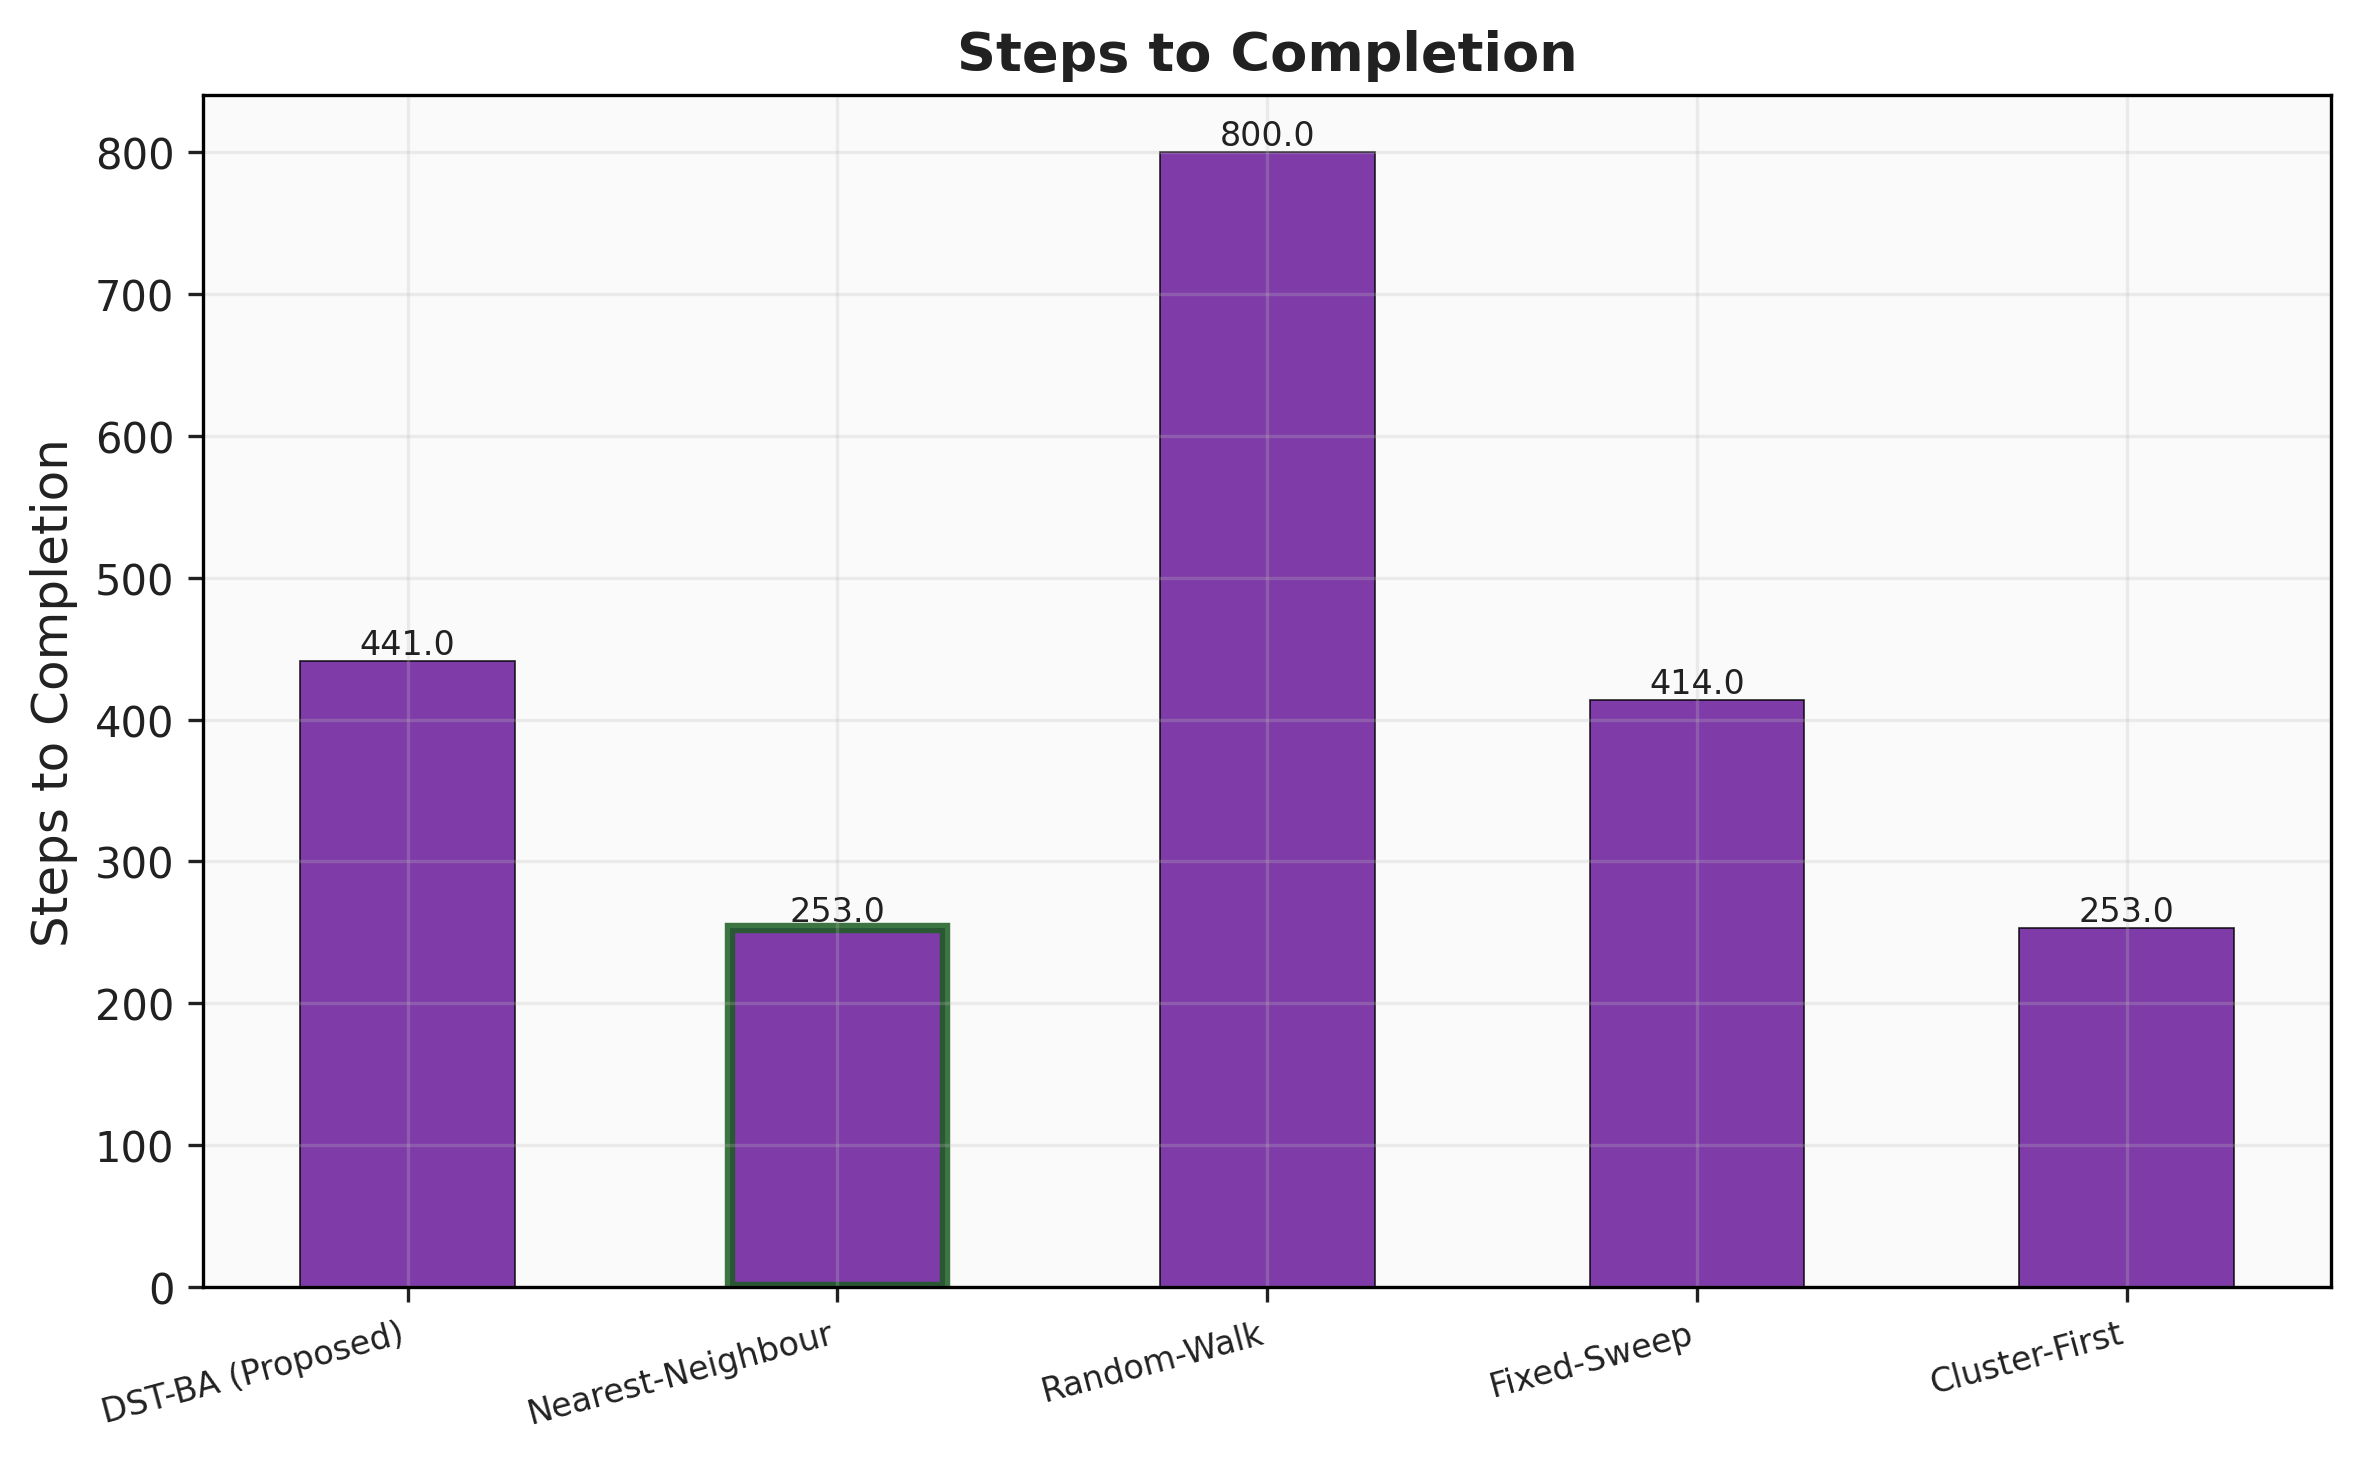
\includegraphics[width=0.85\textwidth]{figures/compare_steps.png}
\caption{Mission steps comparison. DST-BA completes in 441 steps --- fewer than Random-Walk (800) and comparable to Fixed-Sweep (414), while NN/CF use fewer steps due to their unrealistic instantaneous-collection assumption.}
\label{fig:cmp_steps}
\end{figure}

\begin{figure}[htbp]
\centering
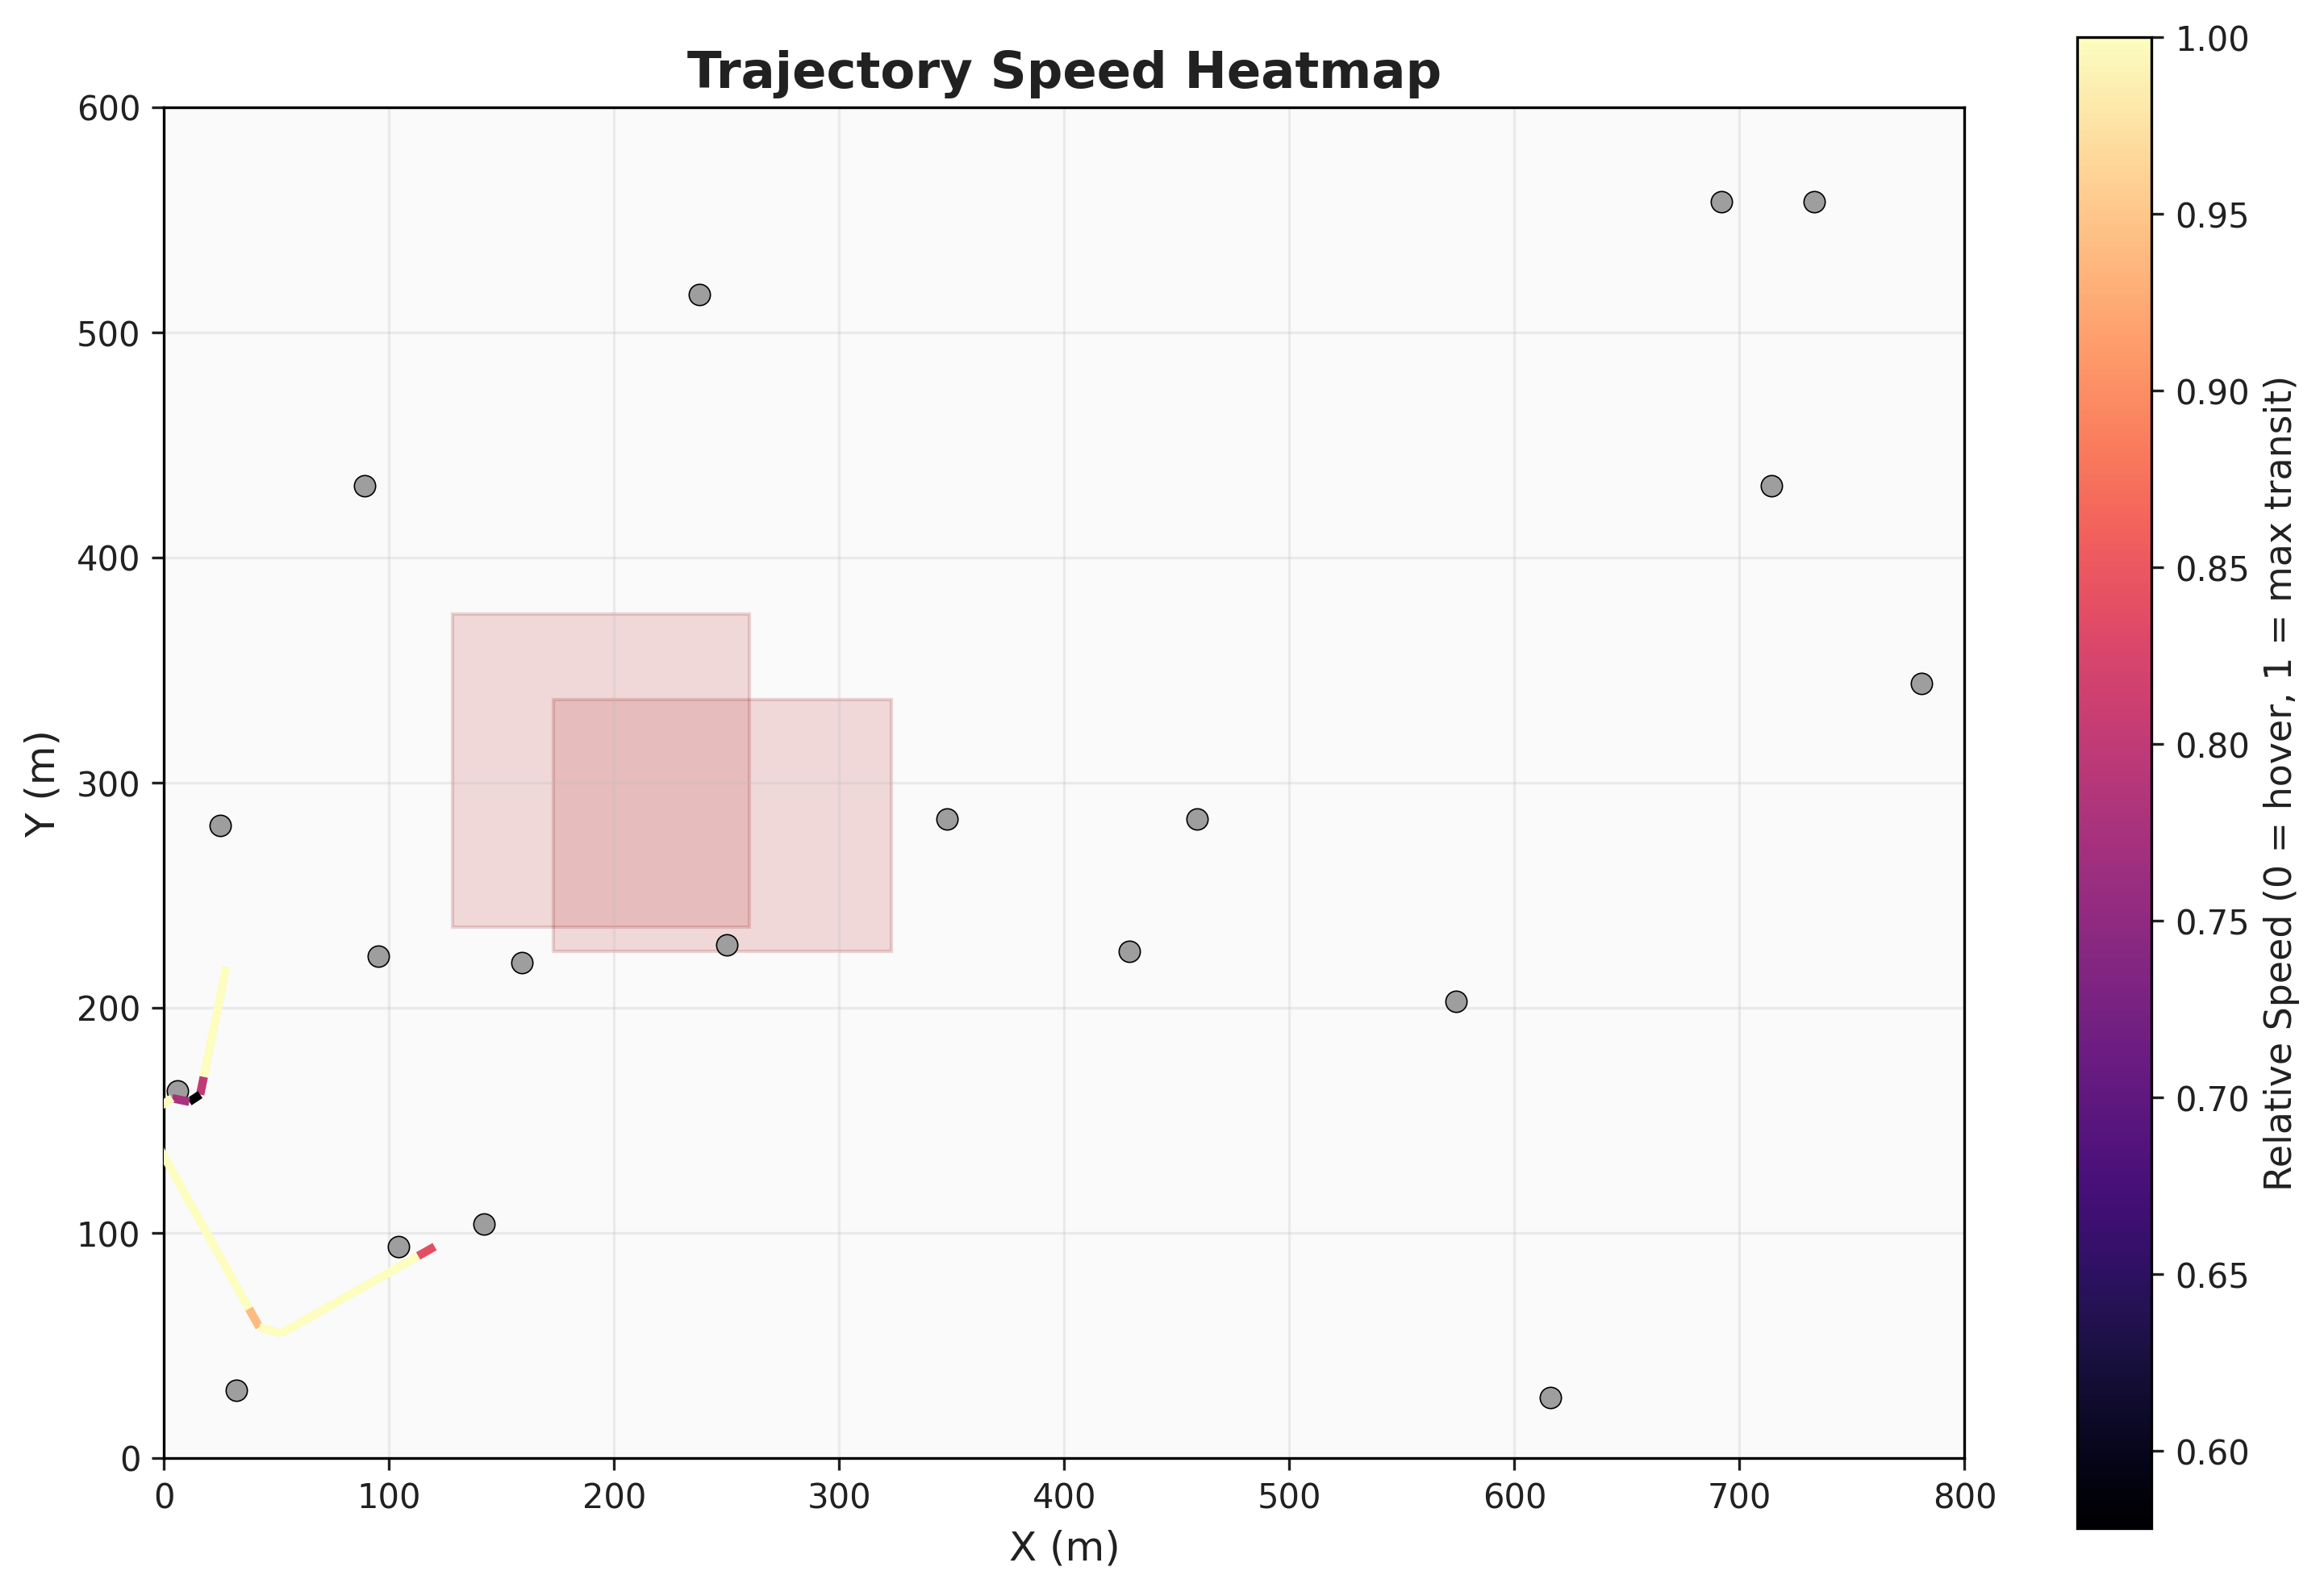
\includegraphics[width=0.85\textwidth]{figures/trajectory_heatmap.png}
\caption{Trajectory heatmap showing UAV dwell time across the operational area. Darker regions indicate longer hover duration for data collection.}
\label{fig:heatmap}
\end{figure}

\begin{figure}[htbp]
\centering
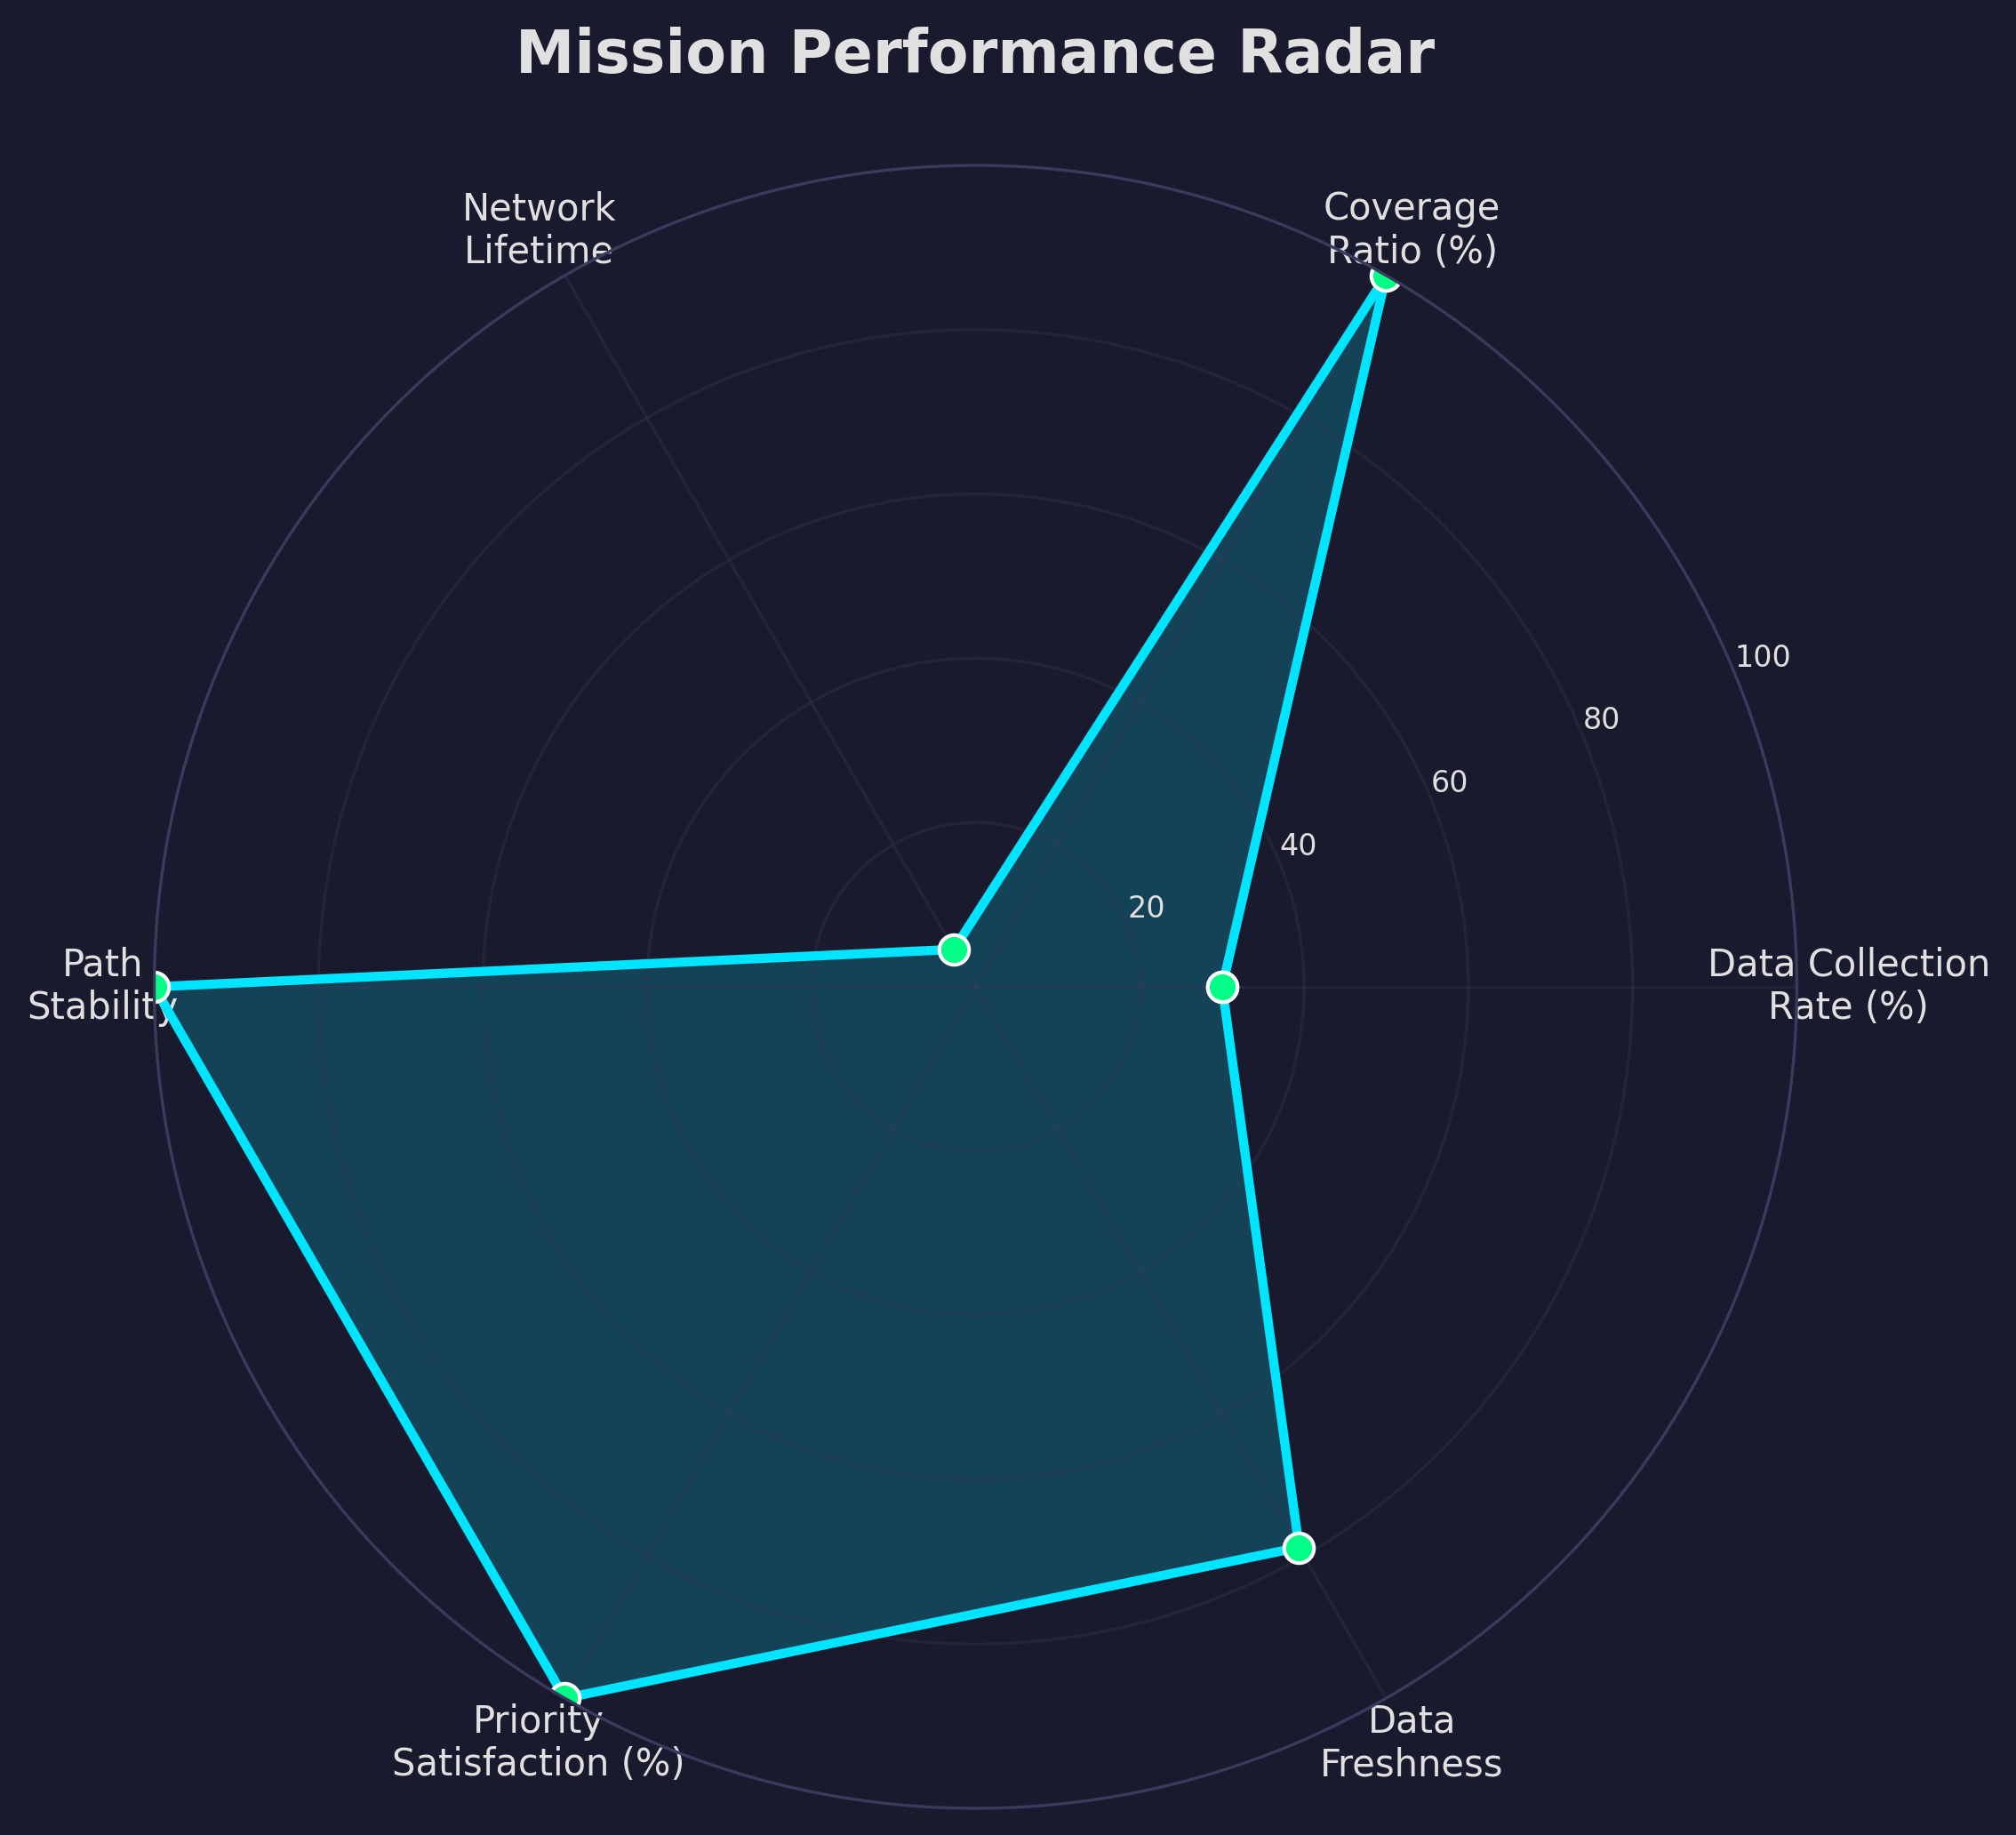
\includegraphics[width=0.75\textwidth]{figures/radar_chart.png}
\caption{Multi-dimensional radar chart comparing DST-BA performance across six normalized metrics: coverage, energy efficiency, data quality, speed, stability, and priority satisfaction.}
\label{fig:radar}
\end{figure}

\begin{figure}[htbp]
\centering
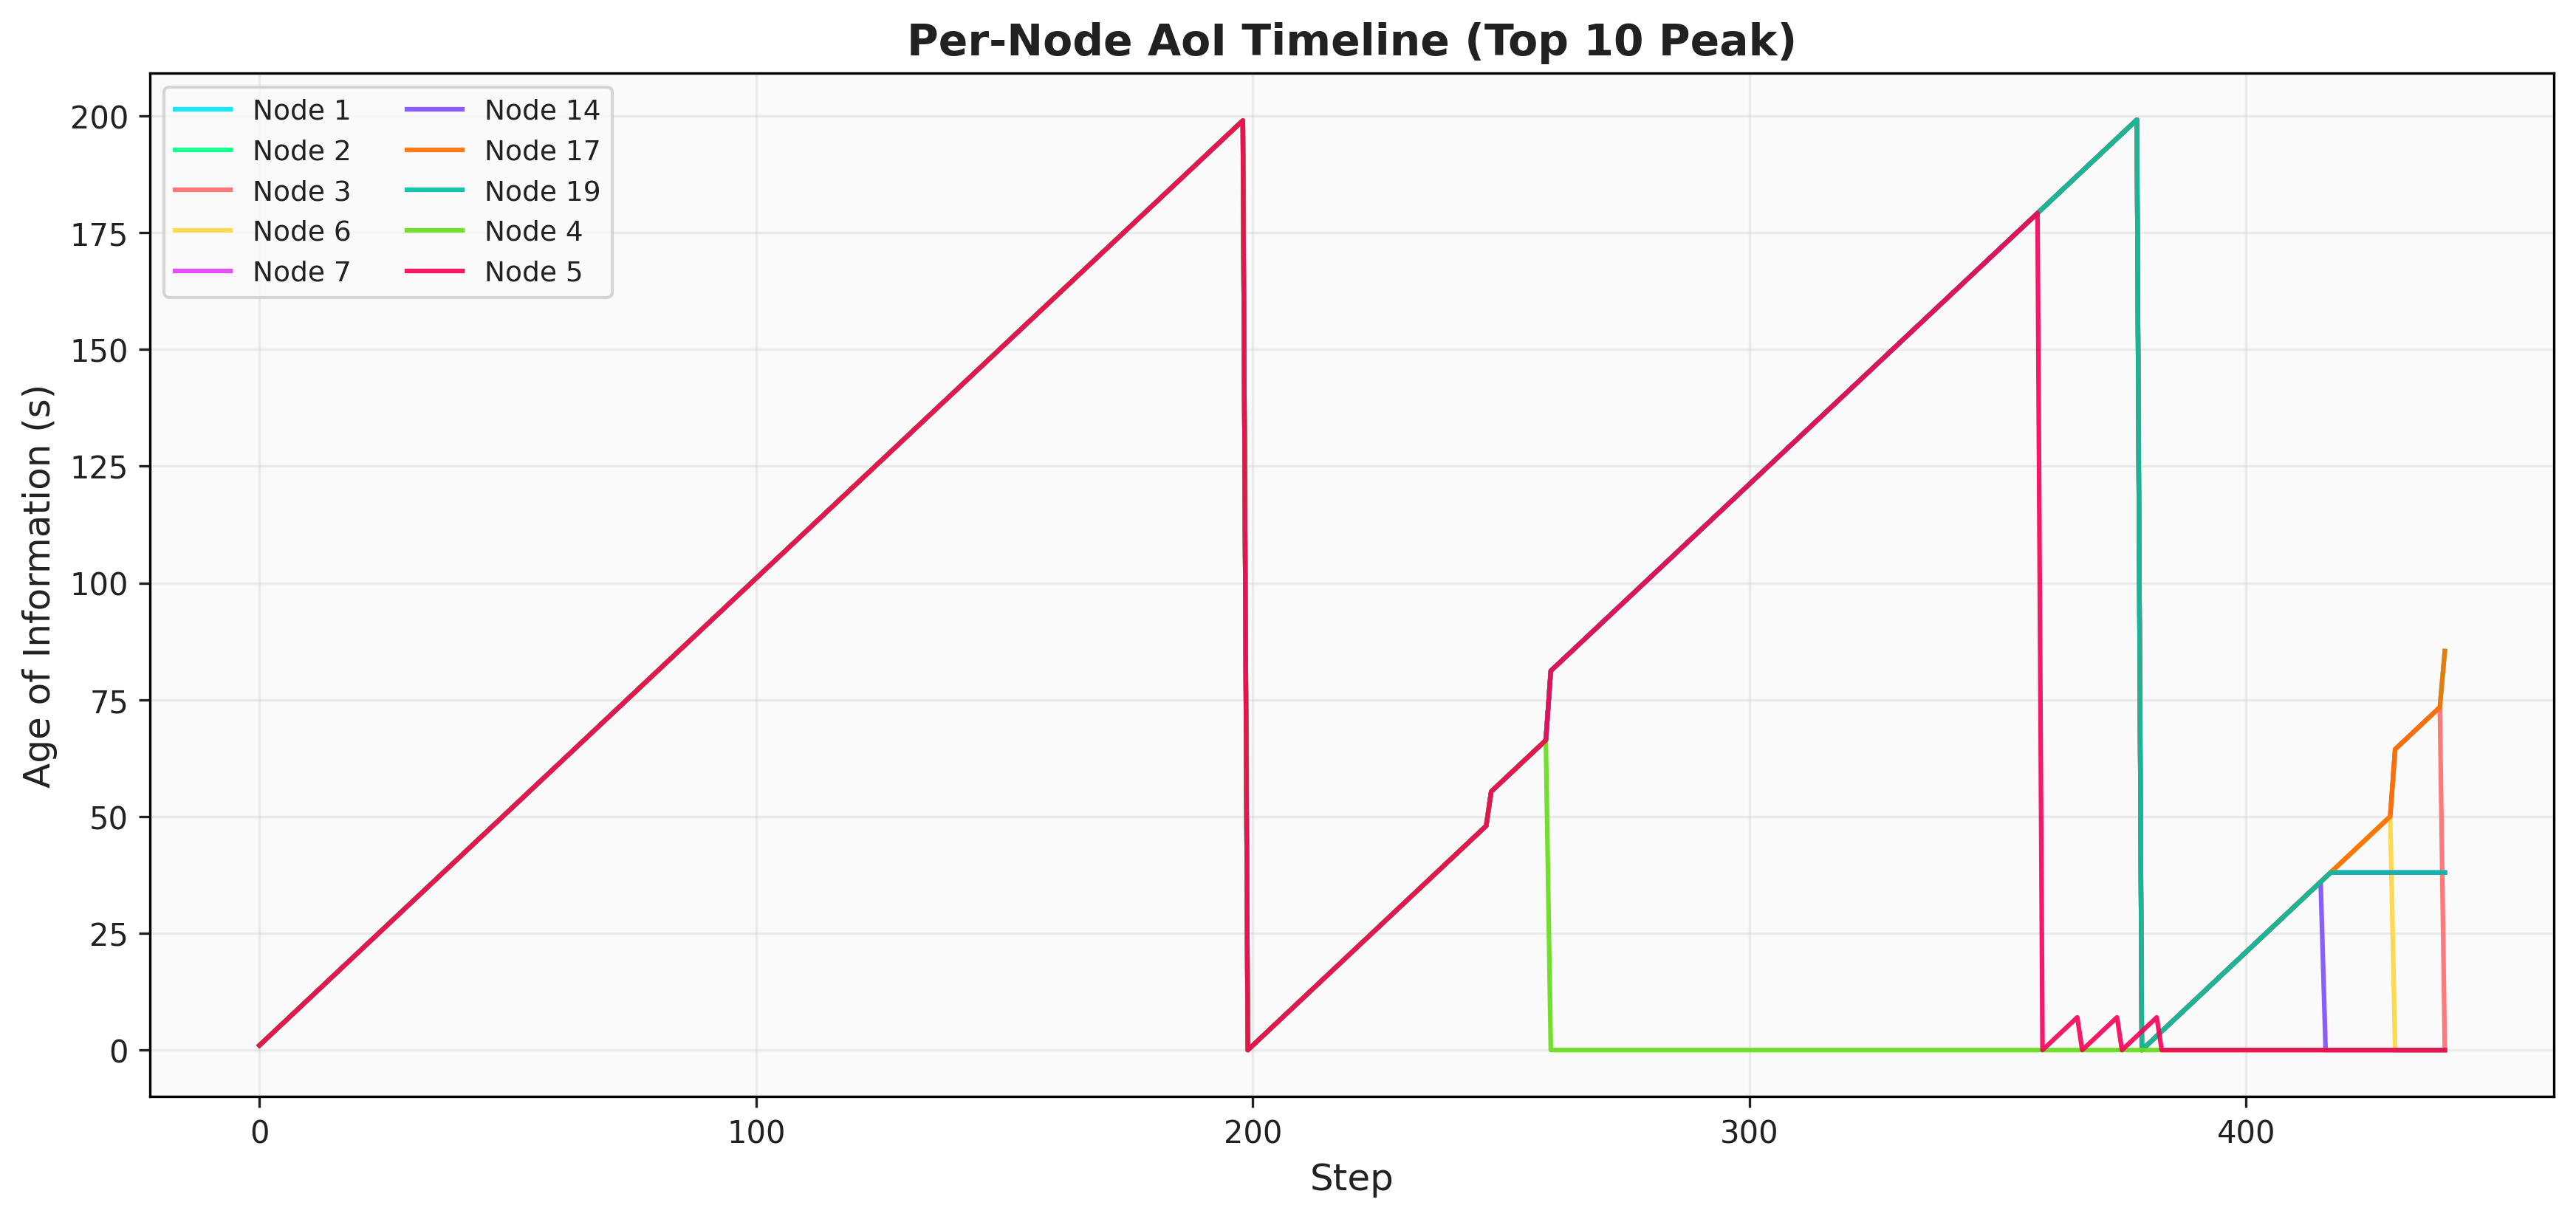
\includegraphics[width=0.85\textwidth]{figures/aoi_timeline.png}
\caption{Age of Information (AoI) timeline for all IoT nodes. Each node's AoI increases linearly until the UAV visits and resets it. Lower final AoI indicates better information freshness.}
\label{fig:aoi}
\end{figure}

\begin{figure}[htbp]
\centering
\begin{minipage}{0.48\textwidth}
\centering
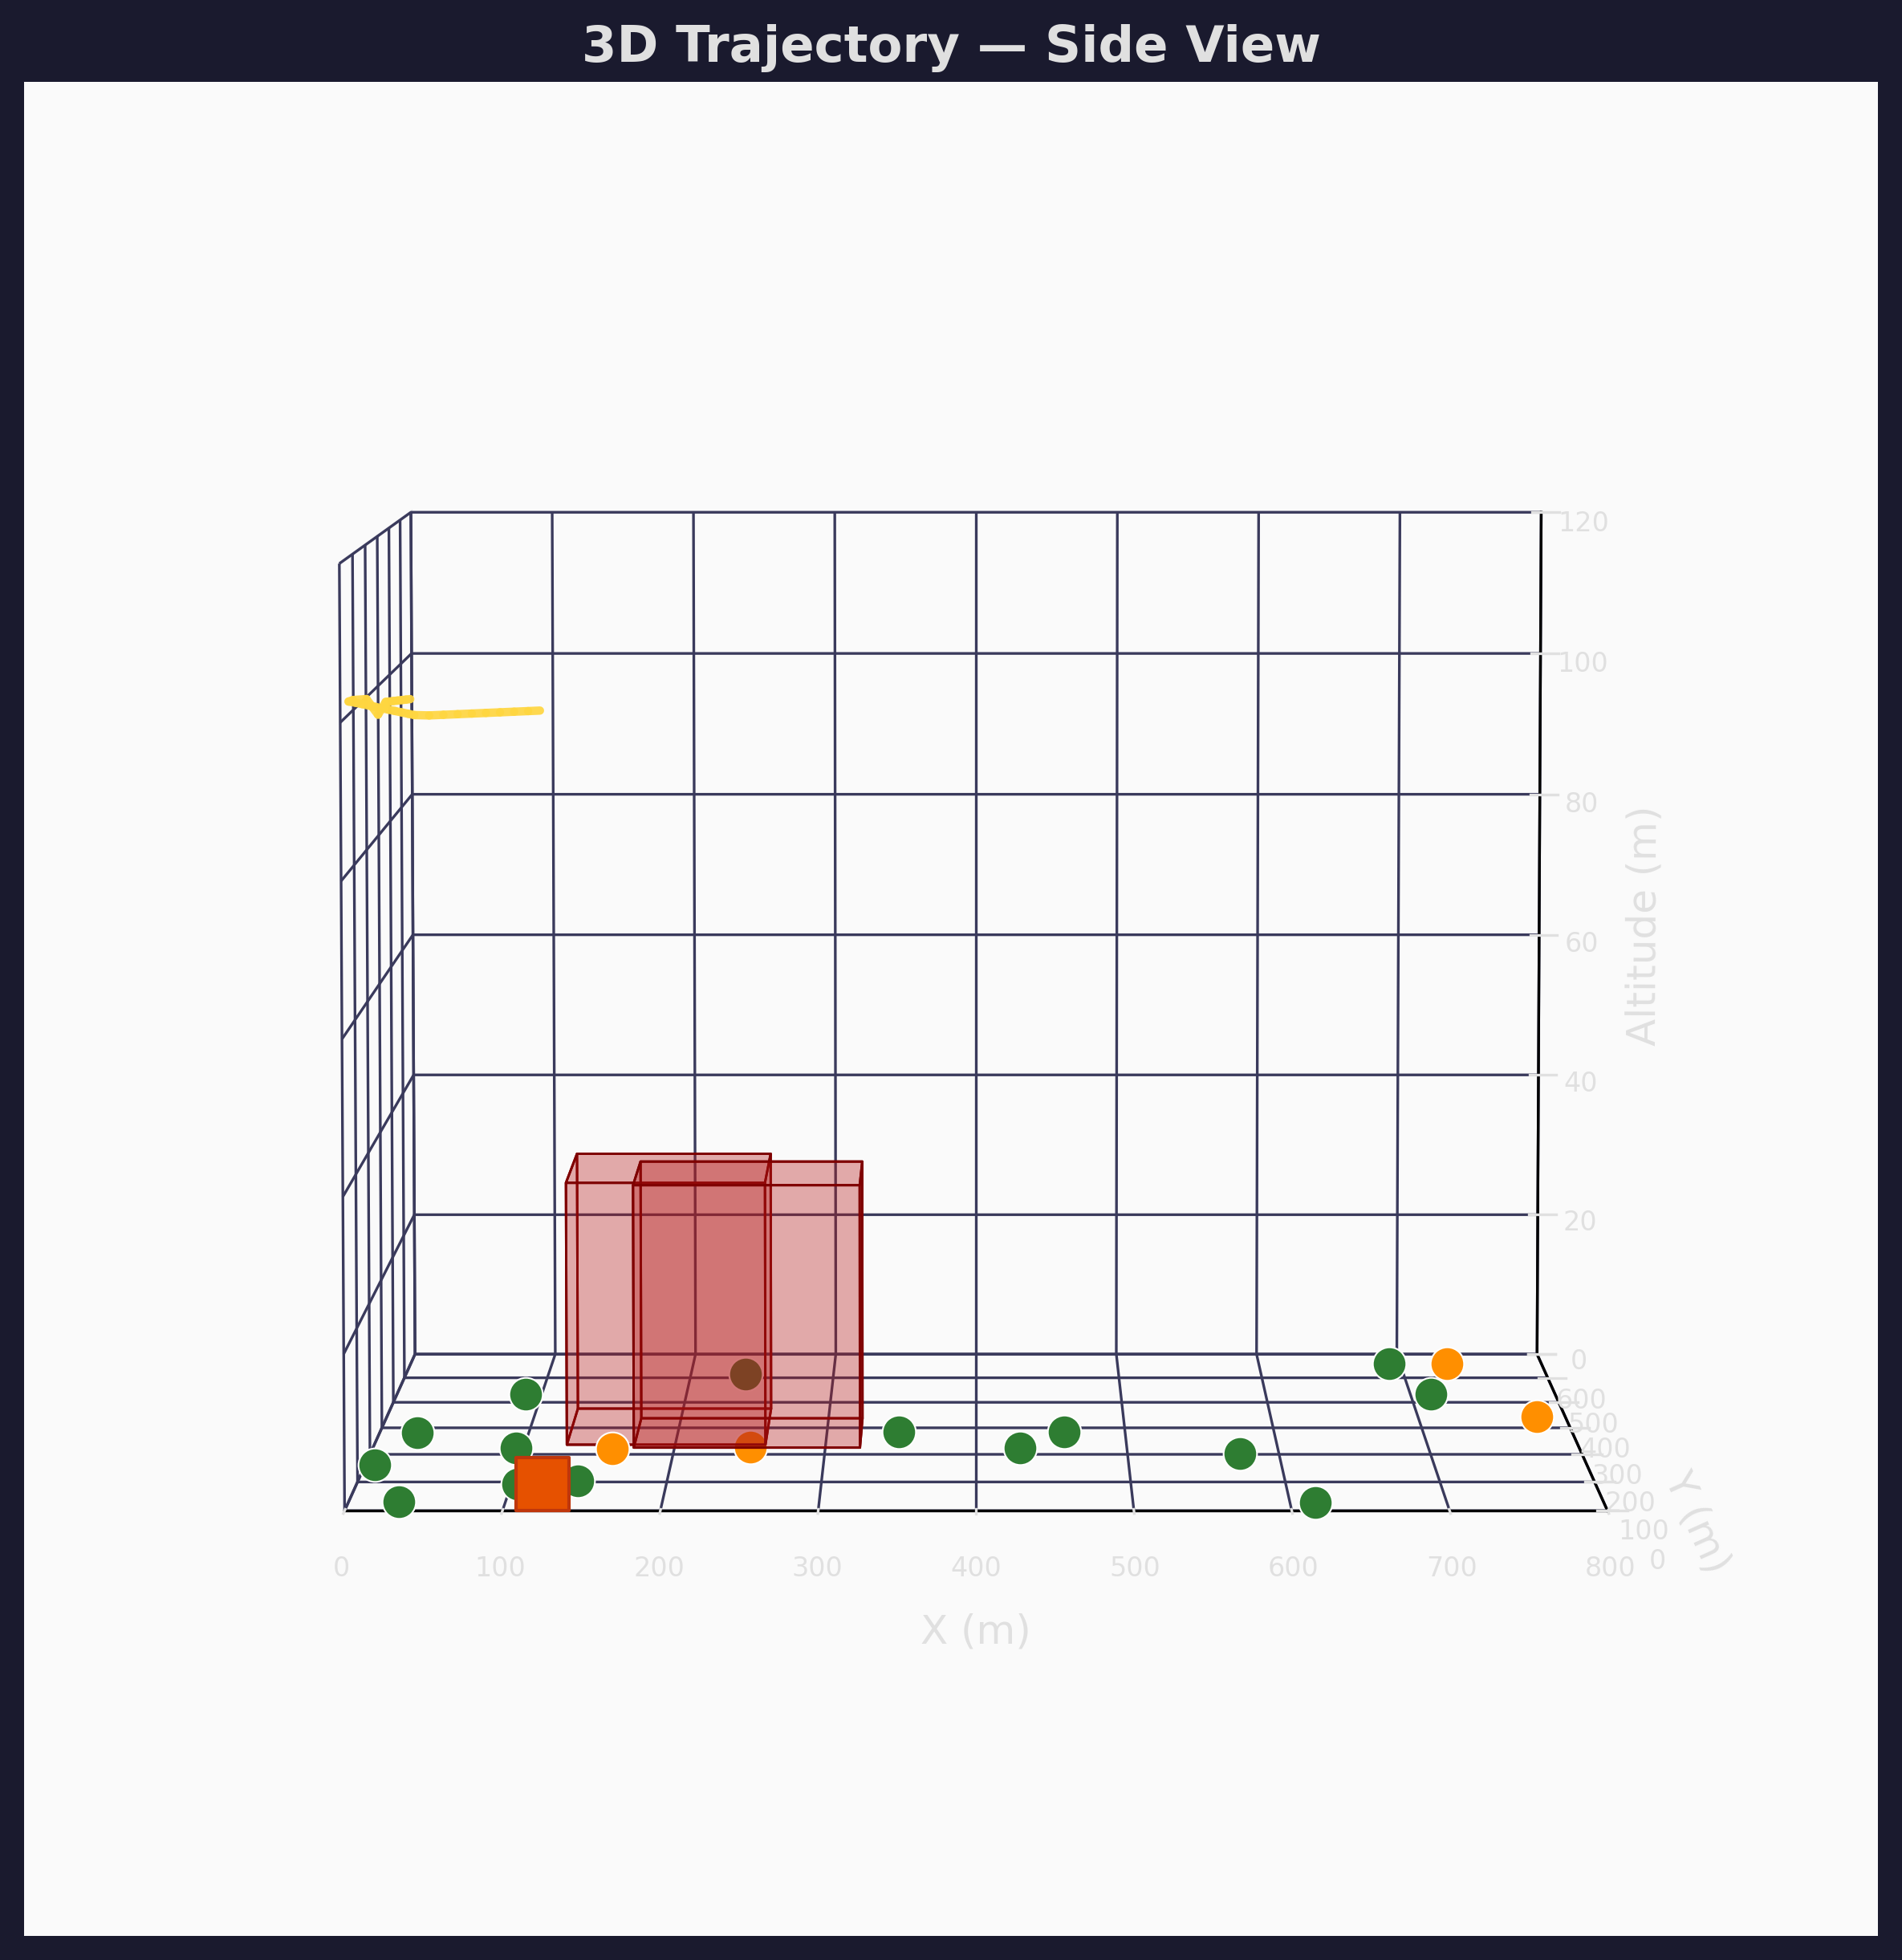
\includegraphics[width=\textwidth]{figures/trajectory_3d_side_view.png}
\caption{Side view of 3D trajectory.}
\label{fig:traj_side}
\end{minipage}
\hfill
\begin{minipage}{0.48\textwidth}
\centering
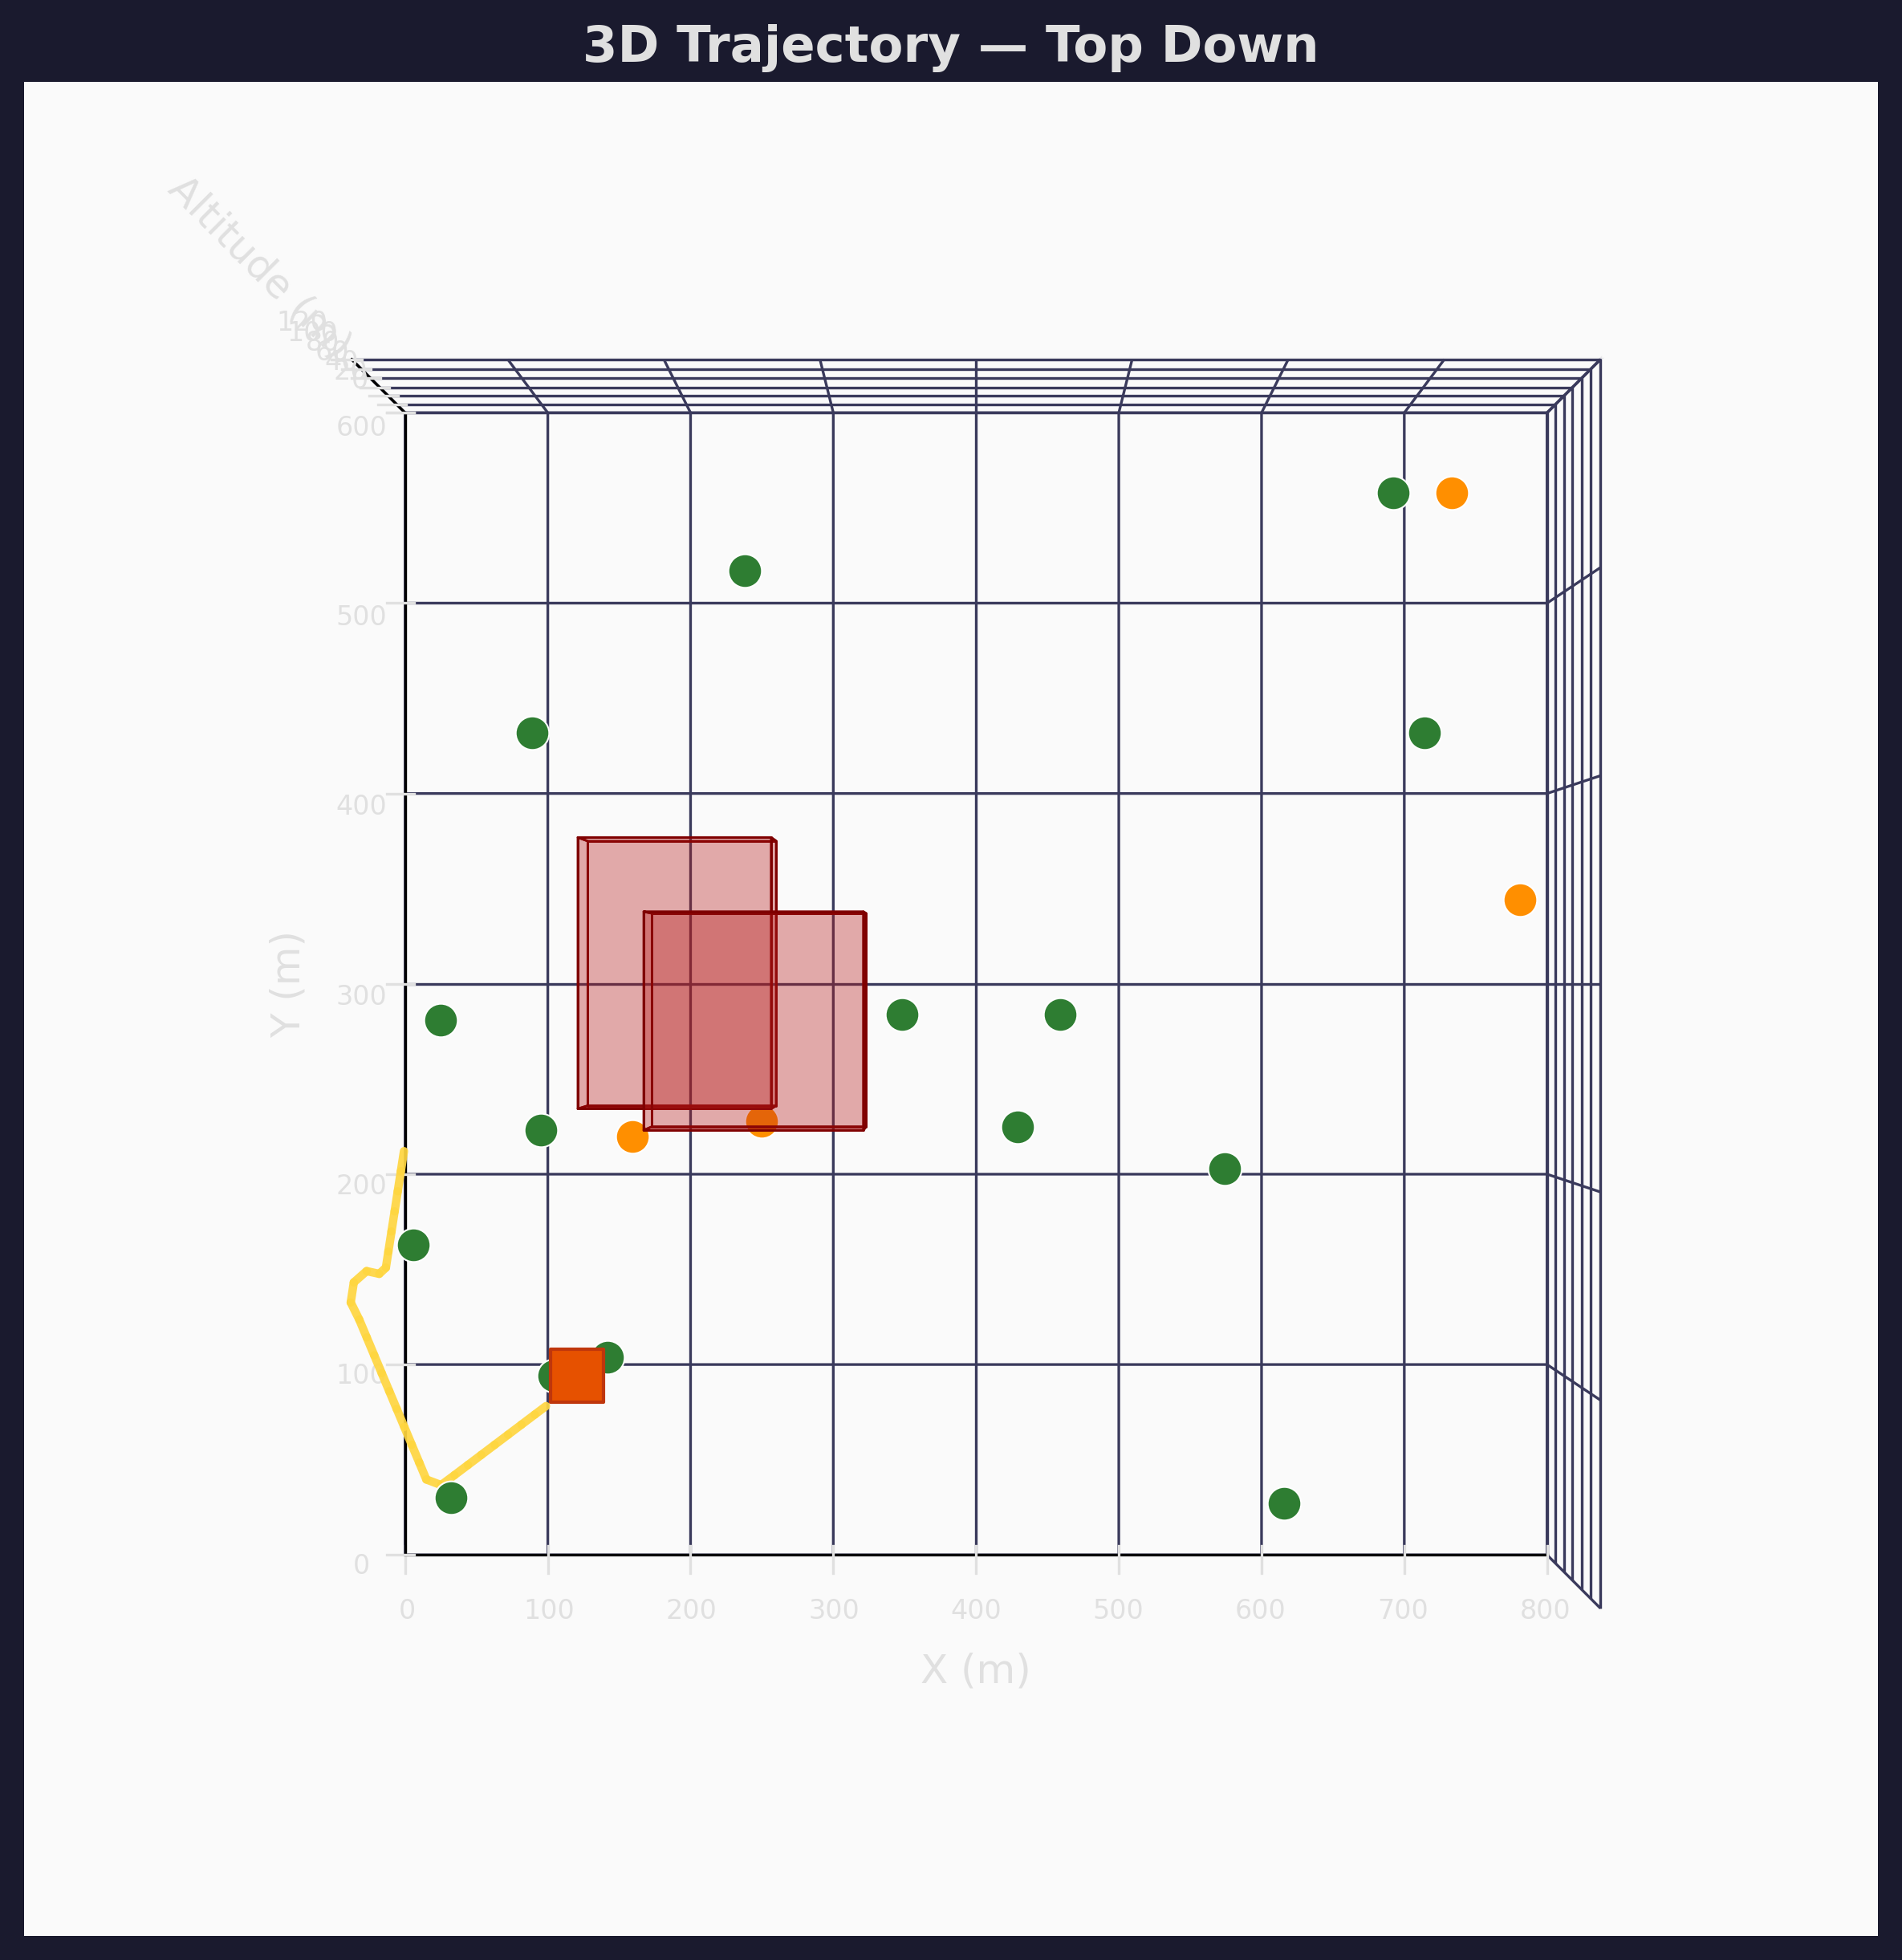
\includegraphics[width=\textwidth]{figures/trajectory_3d_top_down.png}
\caption{Top-down view of 3D trajectory.}
\label{fig:traj_top}
\end{minipage}
\end{figure}

\begin{figure}[htbp]
\centering
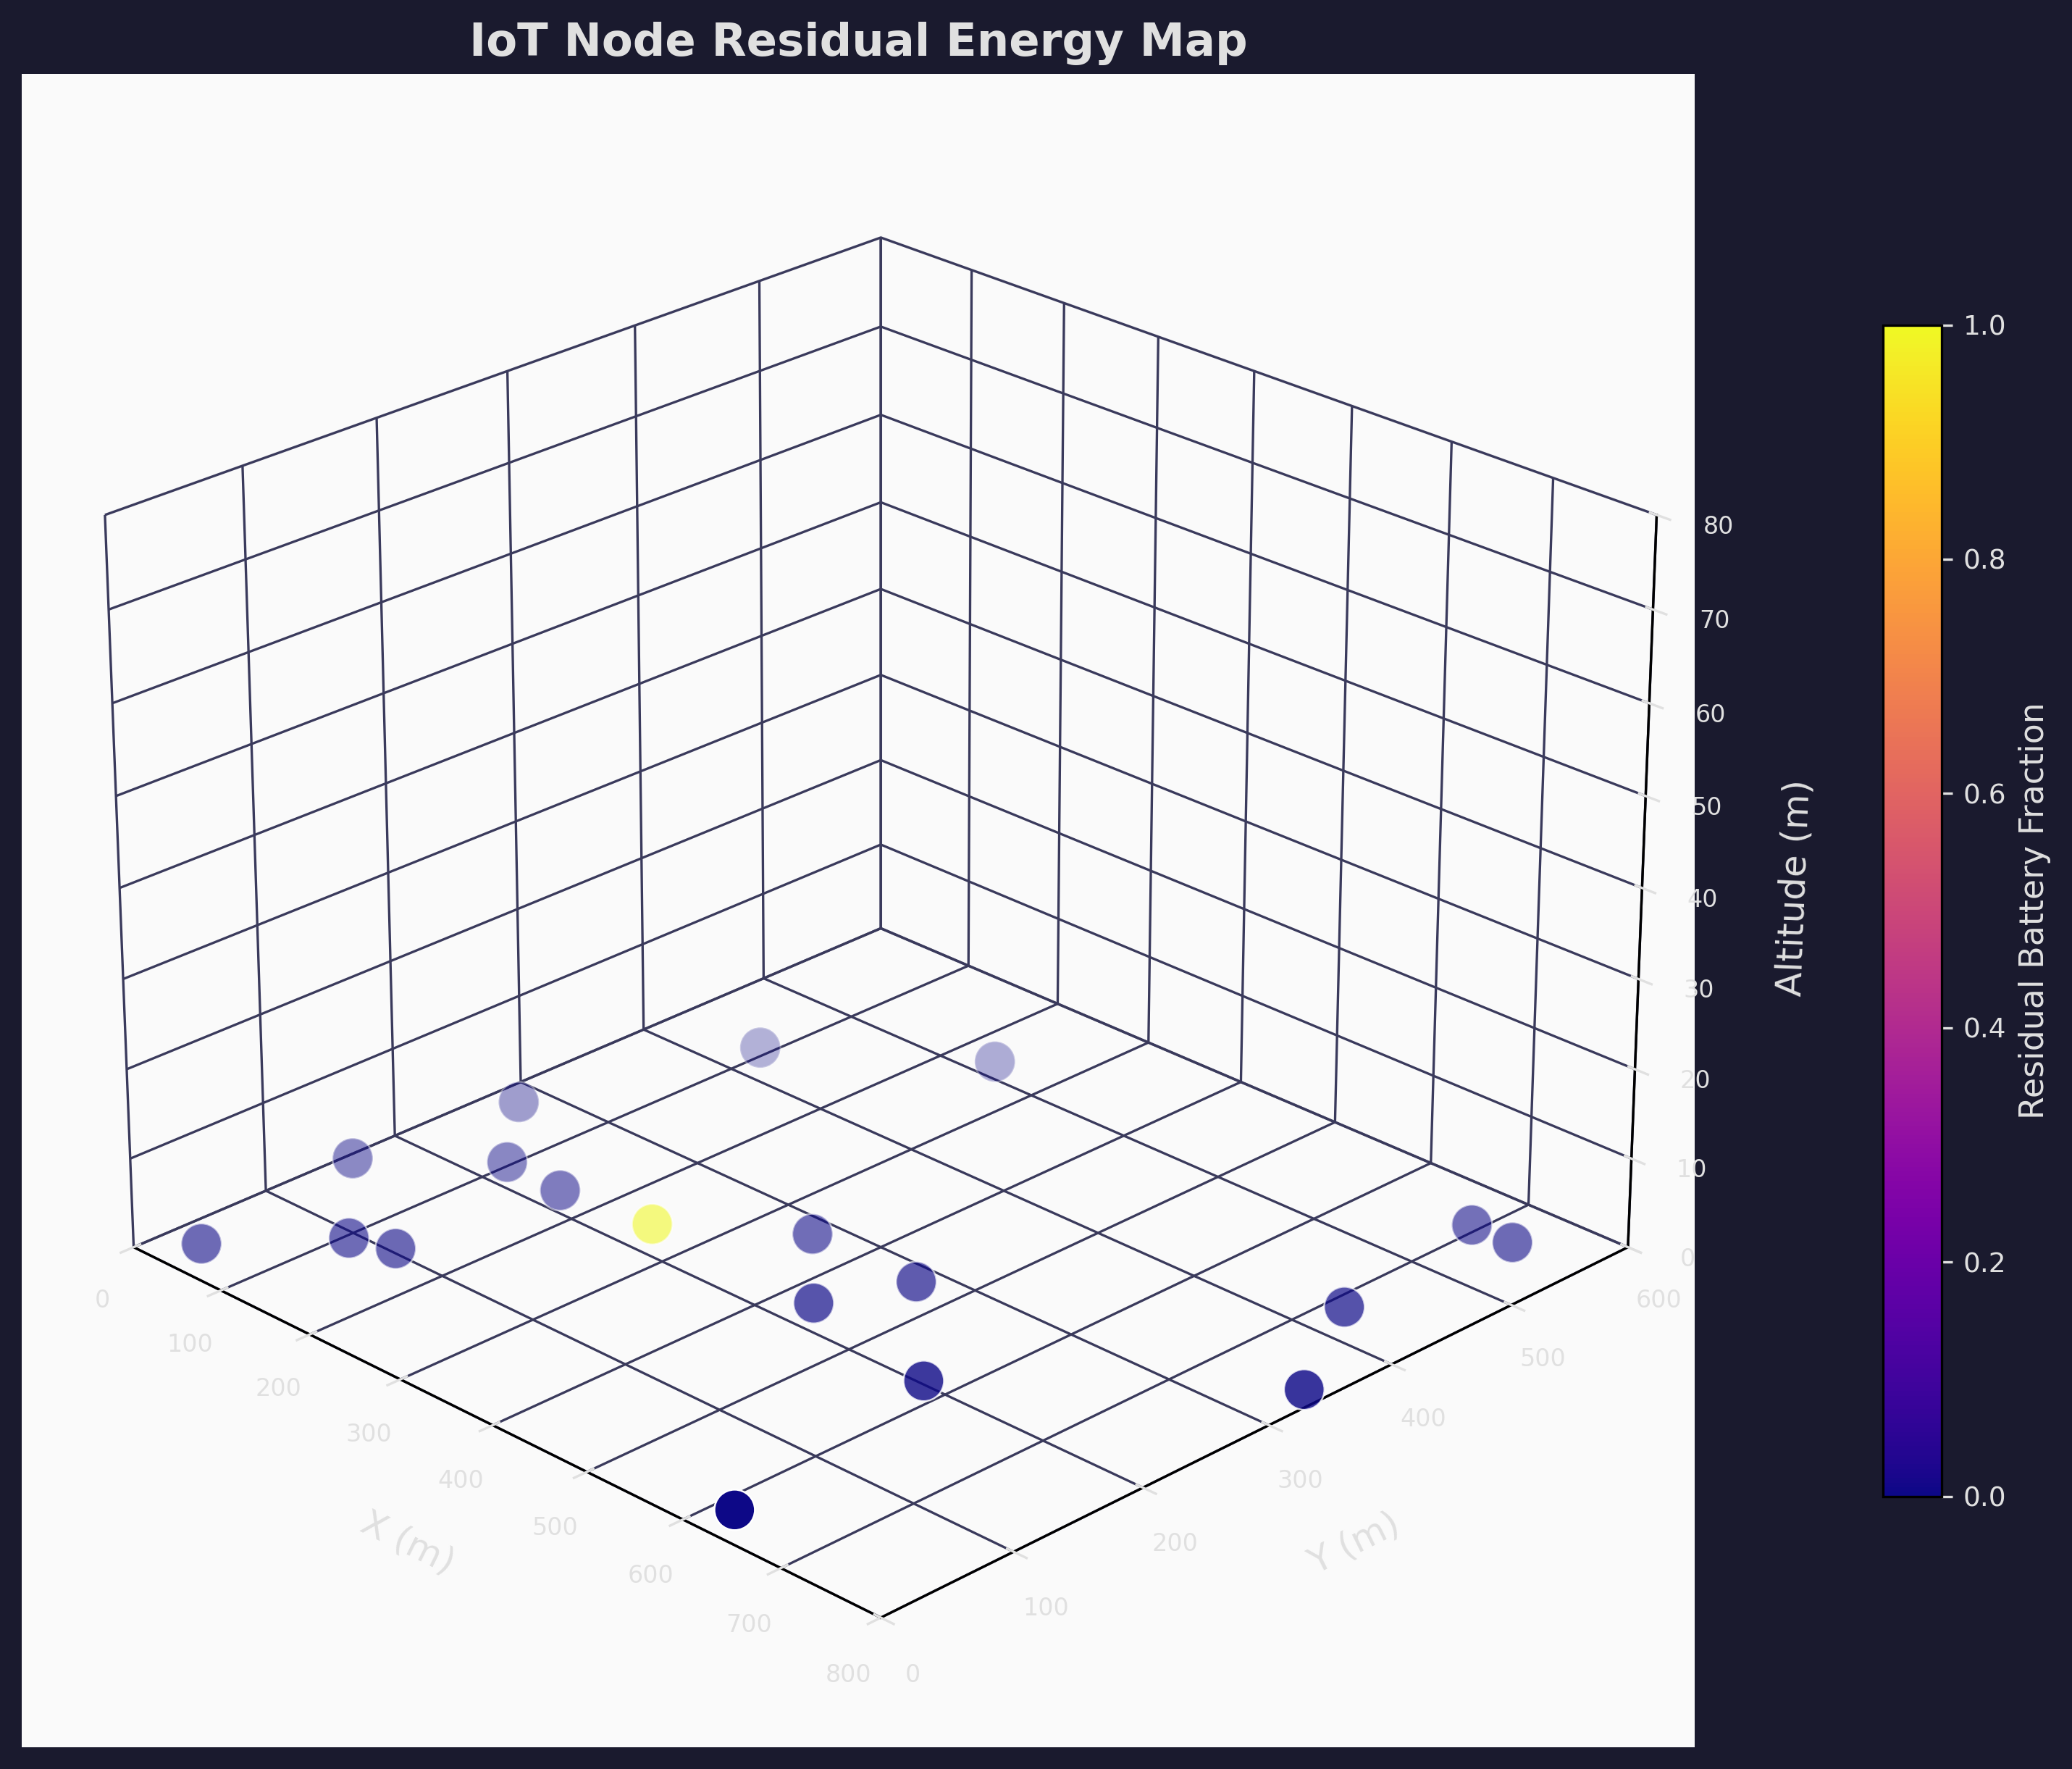
\includegraphics[width=0.85\textwidth]{figures/node_energy_heatmap.png}
\caption{IoT node energy consumption heatmap showing the Heinzelman first-order radio model's per-node energy expenditure during data transmission.}
\label{fig:node_energy}
\end{figure}

\begin{figure}[htbp]
\centering
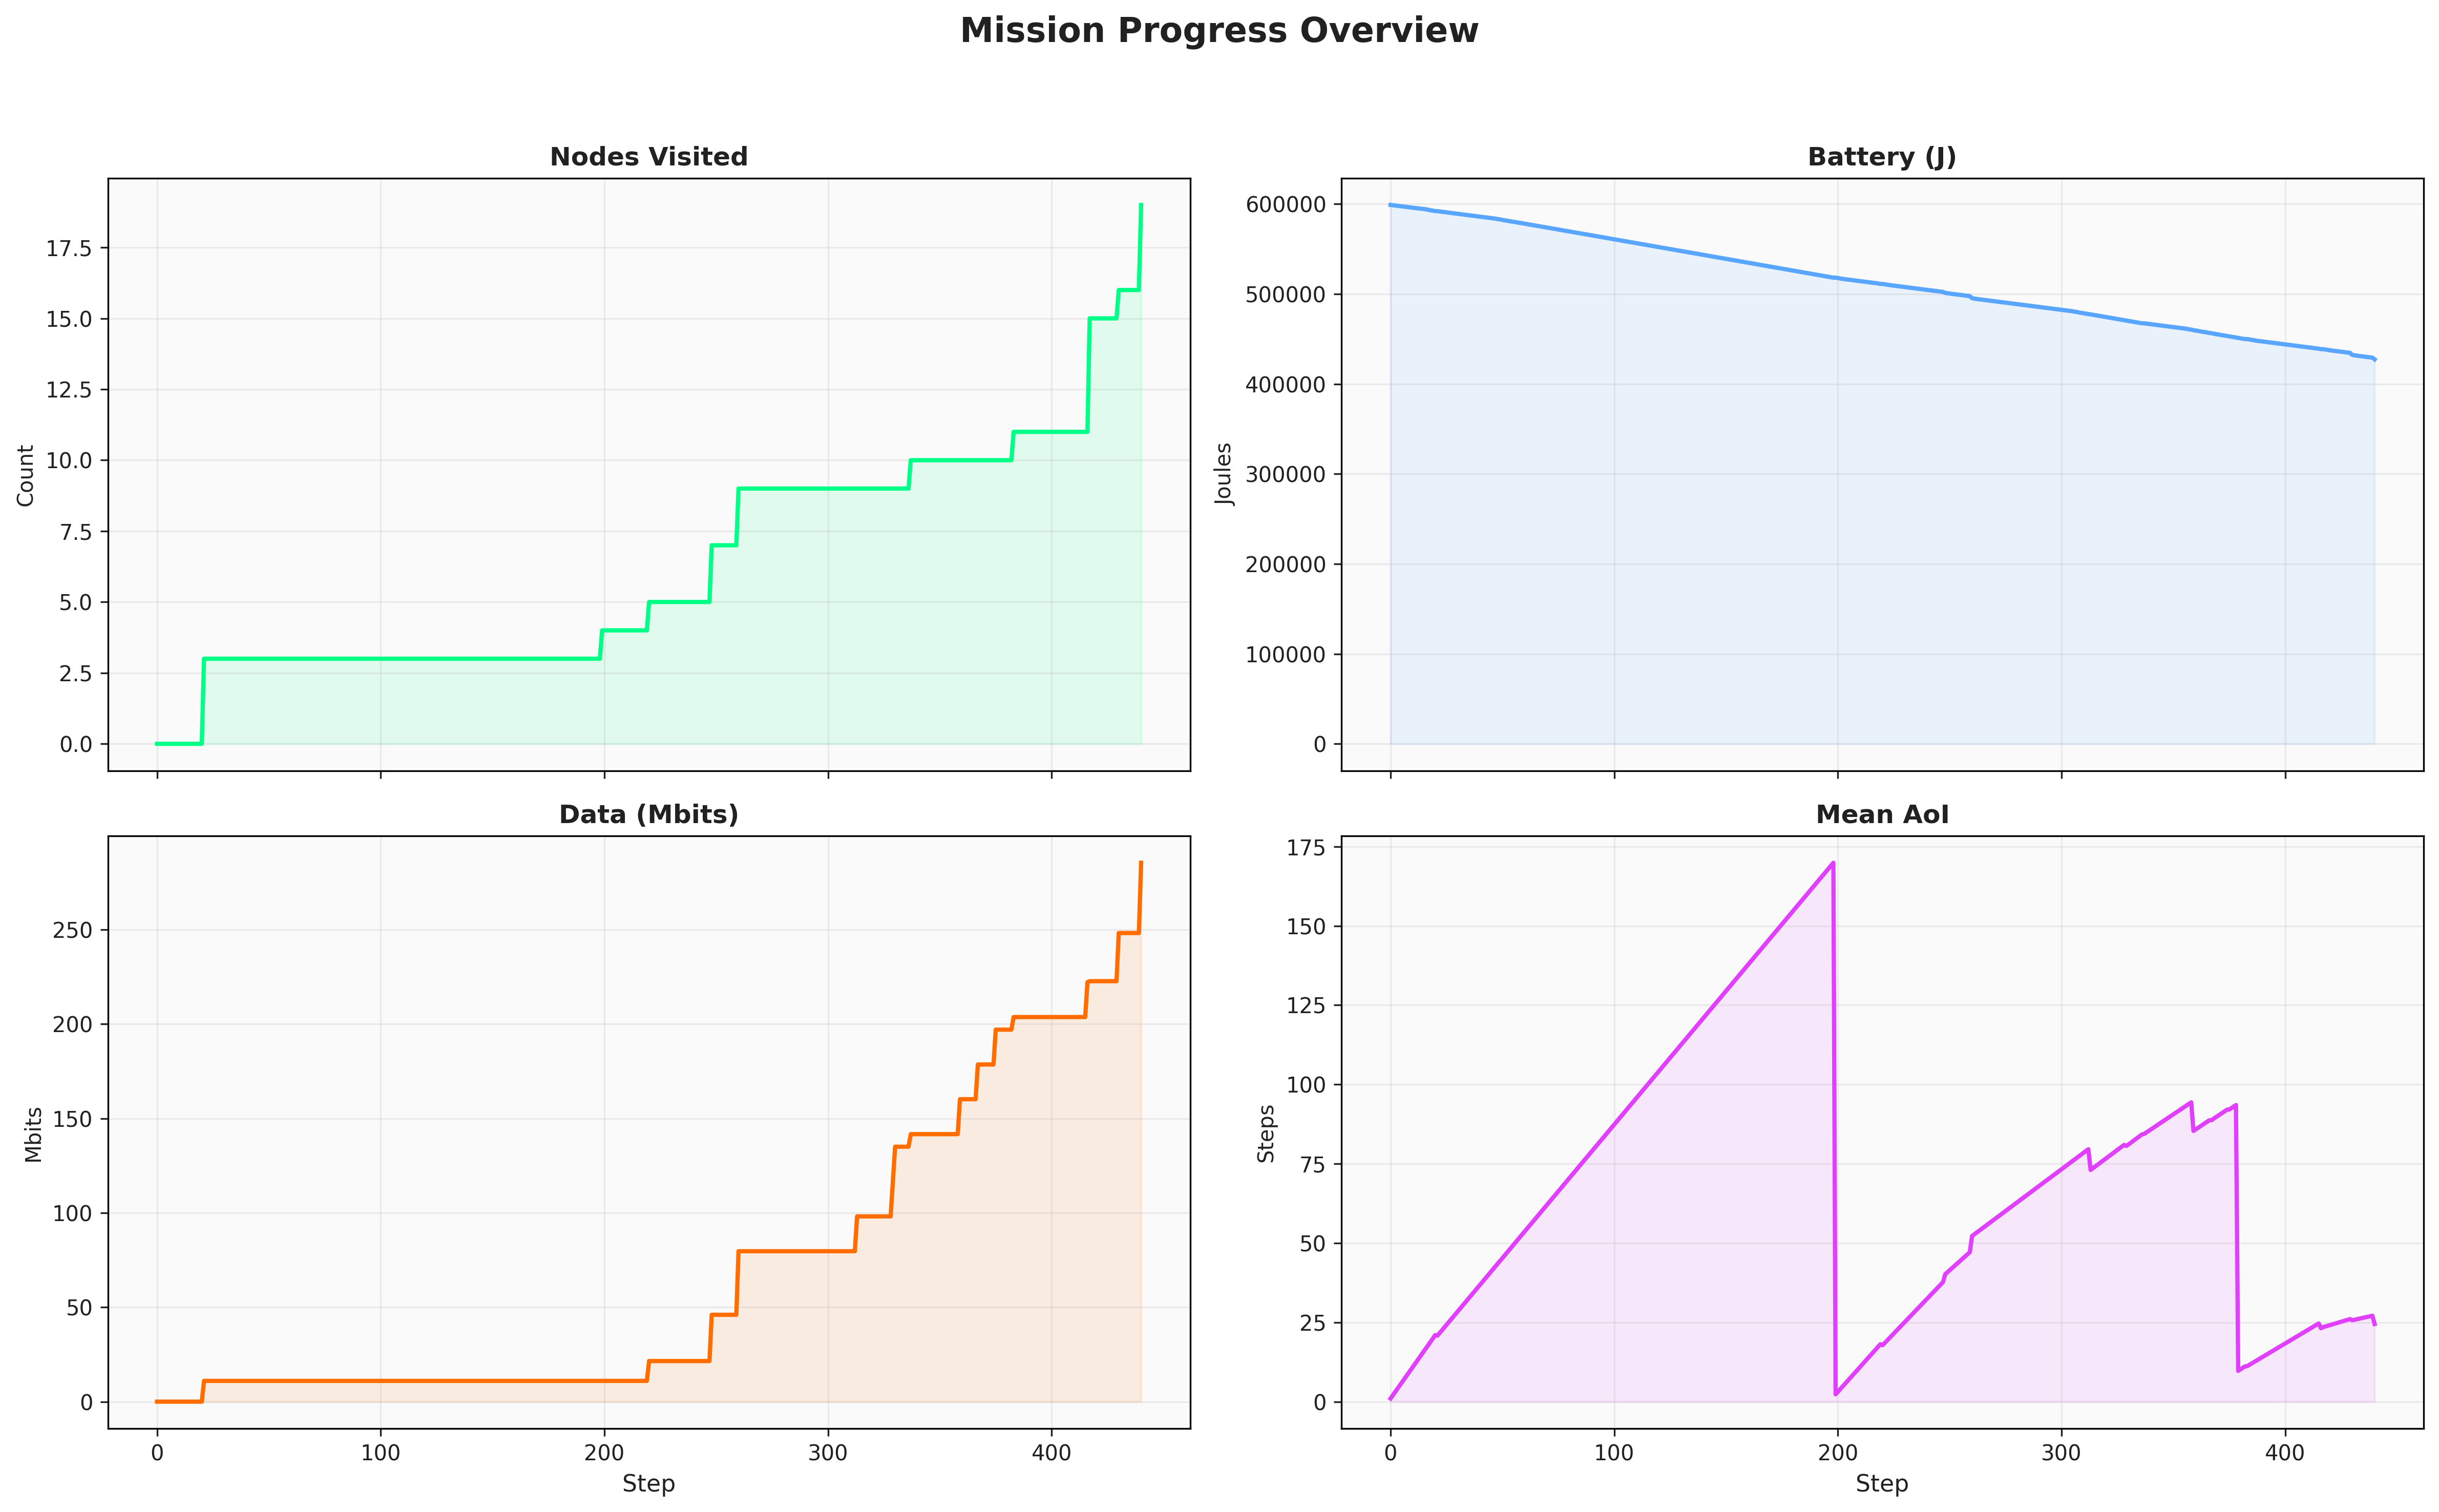
\includegraphics[width=0.95\textwidth]{figures/mission_progress_combined.png}
\caption{Combined mission progress showing (a) cumulative nodes visited, (b) data collected, (c) energy consumed, and (d) coverage ratio over time.}
\label{fig:mission_progress}
\end{figure}


% ════════════════════════════════════════════════════════════════════════════
\chapter{Conclusion and Future Work}
\label{ch:conclusion}
% ════════════════════════════════════════════════════════════════════════════

\section{Summary of Contributions}

This B.Tech project presents DST-BA, a comprehensive framework for autonomous UAV-based data collection from ground IoT sensor networks. The framework integrates eight algorithmic components into a unified pipeline:

\begin{enumerate}
    \item \textbf{Rendezvous Point selection} via greedy dominating set compression ($\sim$70\% waypoint reduction).
    \item \textbf{Semantic multi-feature clustering} with PCA reduction and automatic algorithm selection.
    \item \textbf{GA-based visiting sequence optimization} with time-window constraints and 3D altitude penalties.
    \item \textbf{PCA-GLS path refinement} combining cheapest-arc initialization with penalty-augmented 2-opt.
    \item \textbf{SCA-inspired hover position optimization} for energy-efficient 3D operation.
    \item \textbf{Buffer-aware dynamic service time (DST-BA)} with multi-trial probabilistic sensing.
    \item \textbf{TDMA scheduling} for interference-free single-link communication.
    \item \textbf{Heinzelman first-order radio model} for IoT node battery tracking.
\end{enumerate}

Experimental results demonstrate that DST-BA achieves the \textbf{lowest total energy consumption (172.6~kJ)} and \textbf{lowest energy-per-node (9.1~kJ/node)} compared to four baseline algorithms, while maintaining \textbf{100\% coverage (19/19 nodes)}, zero collisions, 100\% priority satisfaction, and perfect path stability. The UAV completes its mission in only 441 steps with 71.2\% battery residual, confirming the framework's efficiency.

\section{Key Findings}

\begin{enumerate}
    \item \textbf{RP compression is highly effective:} Reducing 19 waypoints to 4--6 RPs directly translates to 13--25\% energy savings over baselines that visit every node.

    \item \textbf{Intelligent routing matters:} The combined GA + PCA-GLS + SCA optimization pipeline produces significantly shorter tours than greedy (NN) or systematic (Sweep) approaches.

    \item \textbf{Channel-aware service is more realistic:} DST-BA's Rician fading based service time computation produces conservative but reliable data collection, unlike baselines that assume ideal instantaneous transfer.

    \item \textbf{Semantic awareness enables priority routing:} The 10-dimensional clustering achieves 100\% priority satisfaction, ensuring critical nodes are served first.

    \item \textbf{The framework is stable and safe:} Zero collisions, near-zero replanning, and 71.2\% battery residual demonstrate production-ready reliability and significant headroom for larger deployments.
\end{enumerate}

\section{Limitations}

\begin{enumerate}
    \item \textbf{Single-UAV constraint:} The current framework considers a single UAV. Multi-UAV coordination would enable larger-scale deployments but introduces additional complexity (task allocation, collision avoidance, spectrum sharing).

    \item \textbf{Static environment:} The simple preset evaluates a static scenario. While the framework supports moving obstacles and dynamic node arrival, these features were not evaluated in the comparative study.

    \item \textbf{Small-scale evaluation:} The experiments use 20 nodes. Scalability to hundreds of nodes may require hierarchical clustering and parallel GA execution.

    \item \textbf{No DRL comparison baseline:} While the GA optimizer performs well, comparison with deep reinforcement learning approaches (PPO, SAC) would further validate the algorithmic choices.
\end{enumerate}

\section{Future Work}

The following extensions are planned for subsequent project phases, organized by development priority:

\subsection{Phase 5: Learning Layer (Immediate Next Phase)}

\begin{enumerate}
    \item \textbf{Deep Reinforcement Learning (DRL) integration:} Replace or augment the GA optimizer with a DRL agent using Proximal Policy Optimization (PPO) or Soft Actor-Critic (SAC) for online adaptive trajectory planning. The state space will encode the 10-dimensional node feature vectors, and the action space will define waypoint selection. This enables real-time adaptation to dynamic environments without recomputing the full 8-stage pipeline.

    \item \textbf{Online learning for service time:} Train a neural network to predict optimal service time $\tau^*$ from observed channel conditions, replacing the current multi-trial Monte Carlo computation with a learned function $\hat{\tau}^*(d, h, K, \text{SNR})$.

    \item \textbf{Transfer learning across environments:} Pre-train the DRL agent on diverse simulated environments (varying node count, obstacle density, and map size) to enable zero-shot deployment on unseen topographies.
\end{enumerate}

\subsection{Scalability and Multi-UAV Extensions}

\begin{enumerate}
    \item \textbf{Multi-UAV coordination:} Extend the framework to support $M$ UAVs ($M \geq 2$) with cooperative trajectory planning, distributed task allocation via auction-based algorithms, and inter-UAV collision avoidance using velocity obstacles.

    \item \textbf{Large-scale evaluation:} Conduct experiments with 100--500 nodes on realistic urban topographies using OpenStreetMap terrain data. Investigate hierarchical clustering (two-level RP compression) and parallel GA execution with island model for scalability.

    \item \textbf{Heterogeneous UAV fleets:} Model UAVs with different battery capacities, sensor payloads, and communication ranges, optimizing task assignment to leverage platform diversity.
\end{enumerate}

\subsection{Hardware and Real-World Validation}

\begin{enumerate}
    \item \textbf{Hardware-in-the-loop (HITL) testing:} Interface the simulation with a ROS2/PX4-based flight controller for Software-In-The-Loop (SITL) testing on a Gazebo simulator, with a planned migration to real DJI Matrice 300 hardware.

    \item \textbf{Digital twin deployment:} Deploy the digital twin map module (already implemented) as a real-time monitoring dashboard that mirrors physical UAV state during field operations.

    \item \textbf{Energy model calibration:} Calibrate the propulsion energy model against real flight data from a quadrotor platform to validate the theoretical blade element momentum theory parameters.
\end{enumerate}

\subsection{Advanced Communication and Sensing}

\begin{enumerate}
    \item \textbf{Non-orthogonal multiple access (NOMA):} Replace TDMA scheduling with NOMA for simultaneous multi-node data collection, leveraging successive interference cancellation to improve spectral efficiency.

    \item \textbf{Reconfigurable intelligent surfaces (RIS):} Model ground-level RIS panels that can enhance UAV-to-node channel quality by steering reflected beams, reducing service time and energy consumption.

    \item \textbf{Energy harvesting:} Model solar-powered UAVs with photovoltaic energy harvesting constraints and battery charging waypoints, enabling perpetual mission planning for continuous IoT monitoring.

    \item \textbf{Adaptive RP refinement:} Implement online RP re-evaluation that dynamically adjusts rendezvous points based on real-time node arrivals and departures in highly dynamic environments.
\end{enumerate}


% ============================================================================
%                              REFERENCES
% ============================================================================

\clearpage
\phantomsection
\addcontentsline{toc}{chapter}{References}
\begin{thebibliography}{99}

\bibitem{gubbi2013iot}
J.~Gubbi, R.~Buyya, S.~Marusic, and M.~Palaniswami, ``Internet of Things (IoT): A vision, architectural elements, and future directions,'' \textit{Future Generation Computer Systems}, vol.~29, no.~7, pp.~1645--1660, 2013.

\bibitem{atzori2010iot}
L.~Atzori, A.~Iera, and G.~Morabito, ``The Internet of Things: A survey,'' \textit{Computer Networks}, vol.~54, no.~15, pp.~2787--2805, 2010.

\bibitem{mozaffari2019tutorial}
M.~Mozaffari, W.~Saad, M.~Bennis, Y.-H.~Nam, and M.~Debbah, ``A tutorial on UAVs for wireless networks: Applications, challenges, and open problems,'' \textit{IEEE Communications Surveys \& Tutorials}, vol.~21, no.~3, pp.~2334--2360, 2019.

\bibitem{zeng2019accessing}
Y.~Zeng, Q.~Wu, and R.~Zhang, ``Accessing from the sky: A tutorial on UAV communications for 5G and beyond,'' \textit{Proceedings of the IEEE}, vol.~107, no.~12, pp.~2327--2375, 2019.

\bibitem{zeng2019energy}
Y.~Zeng, J.~Xu, and R.~Zhang, ``Energy minimization for wireless communication with rotary-wing UAV,'' \textit{IEEE Transactions on Wireless Communications}, vol.~18, no.~4, pp.~2329--2345, 2019.

\bibitem{kaul2012status}
S.~Kaul, R.~Yates, and M.~Gruteser, ``Real-time status: How often should one update?'' in \textit{Proc. IEEE INFOCOM}, pp.~2731--2735, 2012.

\bibitem{khuwaja2018survey}
A.~A.~Khuwaja, Y.~Chen, N.~Zhao, M.-S.~Alouini, and P.~Dobbins, ``A survey of channel modeling for UAV communications,'' \textit{IEEE Communications Surveys \& Tutorials}, vol.~20, no.~4, pp.~2804--2830, 2018.

\bibitem{aggarwal2020path}
S.~Aggarwal and N.~Kumar, ``Path planning techniques for unmanned aerial vehicles: A review, solutions, and challenges,'' \textit{Computer Communications}, vol.~149, pp.~270--299, 2020.

\bibitem{wu2018common}
Q.~Wu and R.~Zhang, ``Common throughput maximization in UAV-enabled OFDMA systems with delay consideration,'' \textit{IEEE Transactions on Communications}, vol.~66, no.~12, pp.~6614--6627, 2018.

\bibitem{bouhamed2020uav}
O.~Bouhamed, H.~Ghazzai, H.~Besbes, and Y.~Massoud, ``A UAV-assisted data collection for wireless sensor networks: Autonomous navigation and scheduling,'' \textit{IEEE Access}, vol.~8, pp.~110446--110460, 2020.

\bibitem{liu2019energy}
X.~Liu, Y.~Liu, and Y.~Chen, ``Energy-efficient UAV communication with trajectory optimization,'' \textit{IEEE Transactions on Vehicular Technology}, vol.~68, no.~7, pp.~6909--6921, 2019.

\bibitem{donipati2025tnsm}
S.~Donipati, K.~R.~Pattabiraman, and R.~Vaze, ``UAV-assisted data collection in IoT networks: Rendezvous point optimization with PCA-GLS routing,'' \textit{IEEE Transactions on Network and Service Management}, 2025.

\bibitem{zheng2025tvt}
Z.~Zheng and Y.~Liu, ``Joint UAV trajectory and service time optimization for IoT data collection with probabilistic sensing,'' \textit{IEEE Transactions on Vehicular Technology}, 2025.

\bibitem{wang2022iot}
L.~Wang, H.~Che, K.~Long, S.~Dang, and B.~Champagne, ``Multi-UAV cooperative data collection for IoT networks with TDMA scheduling,'' \textit{IEEE Internet of Things Journal}, vol.~9, no.~19, pp.~18316--18330, 2022.

\bibitem{heinzelman2000leach}
W.~R.~Heinzelman, A.~Chandrakasan, and H.~Balakrishnan, ``Energy-efficient communication protocol for wireless microsensor networks,'' in \textit{Proc. 33rd Annual Hawaii International Conference on System Sciences (HICSS)}, 2000.

\bibitem{al2014los}
A.~Al-Hourani, S.~Kandeepan, and S.~Lardner, ``Optimal LAP altitude for maximum coverage,'' \textit{IEEE Wireless Communications Letters}, vol.~3, no.~6, pp.~569--572, 2014.

\bibitem{garey1979computers}
M.~R.~Garey and D.~S.~Johnson, \textit{Computers and Intractability: A Guide to the Theory of NP-Completeness}. W.~H.~Freeman, 1979.

\bibitem{al2014optimal}
A.~Al-Hourani, S.~Kandeepan, and A.~Jamalipour, ``Modeling air-to-ground path loss for low altitude platforms in urban environments,'' in \textit{Proc. IEEE Global Communications Conference (GLOBECOM)}, pp.~2898--2904, 2014.

\end{thebibliography}


% ============================================================================
%                              APPENDIX
% ============================================================================

\appendix
\chapter{List of Abbreviations}

\begin{tabular}{ll}
\toprule
\textbf{Abbreviation} & \textbf{Full Form} \\
\midrule
AoI & Age of Information \\
CF & Cluster-First Route-Second \\
DBSCAN & Density-Based Spatial Clustering of Applications with Noise \\
DQN & Deep Q-Network \\
DRL & Deep Reinforcement Learning \\
DST-BA & Dynamic Service Time with Buffer-Aware scheduling \\
FS & Fixed-Sweep \\
GA & Genetic Algorithm \\
GLS & Guided Local Search \\
GMM & Gaussian Mixture Model \\
IoT & Internet of Things \\
ISAC & Integrated Sensing and Communication \\
KPI & Key Performance Indicator \\
LoS & Line of Sight \\
MINLP & Mixed-Integer Non-Linear Program \\
NLoS & Non Line of Sight \\
NN & Nearest-Neighbour \\
OX & Order Crossover \\
PCA & Principal Component Analysis (also Parallel Cheapest Arc) \\
PCA-GLS & Parallel Cheapest Arc with Guided Local Search \\
PSI & Path Stability Index \\
RP & Rendezvous Point \\
RW & Random Walk \\
SCA & Successive Convex Approximation \\
SNR & Signal-to-Noise Ratio \\
TDMA & Time Division Multiple Access \\
TSP & Travelling Salesman Problem \\
UAV & Unmanned Aerial Vehicle \\
\bottomrule
\end{tabular}


\end{document}
